\documentclass[11pt,a4paper,titlepage,
chapterprefix,headsepline,parskip,pdftex,
,pointlessnumbers,bibtotoc]{scrbook}

%%% Absätze bei tieferen Ebenen einschalten
\makeatletter %% Sonderbedeutung von @ aufheben
\renewcommand{\paragraph}{\@startsection
   {paragraph} % name
   {4} % ebene
   {0mm} % einzug
   {-\baselineskip} % vorabstand
   {0.1\baselineskip} % nachabstand
   {\normalfont\normalsize\bfseries}} % stil
\makeatother %% Sonderbedeutung von @ wieder

\makeatletter %% Sonderbedeutung von @ aufheben
\renewcommand{\subparagraph}{\@startsection
   {subparagraph} % name
   {5} % ebene
   {0mm} % einzug
   {-\baselineskip} % vorabstand
   {0.1\baselineskip} % nachabstand
   {\normalfont\normalsize\bfseries}} % stil
\makeatother %% Sonderbedeutung von @ wieder

\usepackage{setspace}
\onehalfspacing

\usepackage[pdftex]{graphicx}

%my imports:
\usepackage{subfig}
\usepackage{afterpage}
\usepackage{algorithmic}
\usepackage[para,online,flushleft]{threeparttable} % Custom captions under/above floats in tables or figures.
\usepackage[chapter]{algorithm}
\usepackage{mathtools}
\usepackage{float}
\usepackage{listings}
\usepackage{graphicx}
\usepackage{boxedminipage}
\usepackage{framed}
\usepackage{amssymb}
\usepackage{amsmath} % Includes \nobreakdash and other stuff.
\usepackage{tabulary}
\usepackage[pdftex]{colortbl}
%my theorems:
%\newtheorem{definition}{Definition}
\newtheorem{definition}{Definition}
\numberwithin{definition}{chapter}

% for colours
\usepackage[pdftex]{color}

\usepackage[colorlinks=true,
    linkcolor=blue,
    citecolor=blue,
    pagecolor=blue,
    urlcolor=blue,
    breaklinks=true,
    bookmarksnumbered=true,
    hypertexnames=false,
    pdfpagemode=UseOutlines,
    pdfview=FitH,
    plainpages=false,
    pdfpagelabels,
    bookmarks=true,
    linktocpage=true]{hyperref}


% To-Do Befehl
\newcommand{\todo}[1]{\textcolor{red}{\textbf{To-Do:} #1}}

% Interner-Link-Befehl
\newcommand{\internerLink}[1]{\hyperref[#1]
{Siehe \ref*{#1}~\nameref{#1} auf S.~\pageref{#1}}}

% Interner-Link-Befehl 2
\newcommand{\ffinternerLink}[1]{\hyperref[#1]
{Siehe S.~\pageref{#1}ff}}

% Interner-Link-Befehl x
\newcommand{\xinternerLink}[1]{\hyperref[#1]
{\ref*{#1}~\nameref{#1} auf S.~\pageref{#1}}}


%%% continous footnote
\newcounter{cfootnotecounter}
\newcommand{\cfootnote}[1]{\stepcounter{cfootnotecounter}
\footnote[\value{cfootnotecounter}]{#1}}

%%% Bild Befehle
\newcommand{\bild}[3]{\begin{figure}[htb] \begin{center}
\includegraphics{#1}
\caption{#2} \label{#3} \end{center} \end{figure}}

\newcommand{\bildTabelle}[3]{\begin{table}[htb] \begin{center}
\includegraphics{#1}
\caption{#2} \label{#3} \end{center} \end{table}}

\newcommand{\bildE}[5]{\begin{figure}[hb] \begin{center}
\includegraphics[height=#2, angle=#3]{#1}
\caption{#4} \label{#5} \end{center} \end{figure}}

\newcommand{\tabelle}[3]{\begin{table}[htb] \begin{center}
\input{#1}
\caption{#2} \label{#3} \end{center} \end{table}}

\flushbottom

% change page settings
\setlength{\hoffset}{0mm} \setlength{\voffset}{0mm}
% \setlength{\evensidemargin}{14.6mm}
% \setlength{\oddsidemargin}{14.6mm}
\setlength{\topmargin}{-20mm}
\setlength{\headheight}{15mm} \setlength{\headsep}{9mm}
\setlength{\textheight}{242mm} \setlength{\textwidth}{145mm}
\setlength{\footskip}{10mm}
%%% Nachfolgendes nicht notwendig wg. Klassenoption parskip
%\setlength{\parskip}{3ex plus0.5ex minus0.5ex}
%\setlength{\parindent}{0mm}

%%% Abstände von float-Umgebungen
% \setlength{\textfloatsep}{25pt plus5pt minus5pt}
% \setlength{\intextsep}{25pt plus5pt minus5pt}

%%% Gliederungs-Nummern in den Rand schreiben
\renewcommand*{\othersectionlevelsformat}[1]{%
\llap{\csname the#1\endcsname\autodot\enskip}}

%%% In Kopfzeile nur Kapitel-Text ohne "Kapitel x"
\renewcommand*{\chaptermarkformat}{}

%%% Formatierung von chapter ändern
\setkomafont{chapter}{\Huge}
\RedeclareSectionCommand[beforeskip=50pt]{chapter}
\renewcommand*{\chapterformat}{\LARGE{\chapappifchapterprefix{\ }\thechapter\autodot\enskip}}

%%% Kopfzeile
\usepackage[automark]{scrpage2}

\clearscrheadings \clearscrplain \clearscrheadfoot
\pagestyle{scrheadings}
\ohead{\pagemark}
\ihead{\headmark}
\cfoot{}

%%% Formatierung von Kapitel-Seiten
\renewcommand*{\chapterpagestyle}{scrheadings}

%% Gliederung TOC und Nummerierungstiefe
\setcounter{tocdepth}{\subsubsectionlevel}
\setcounter{secnumdepth}{\subsubsectionlevel}

%%% Schriftarten
\addtokomafont{chapter}{\sffamily}
\addtokomafont{sectioning}{\rmfamily}

% Sprache
\usepackage[german,english]{babel}
% Verwenden von T1 Fonts
\usepackage[T1]{fontenc}
% Eingabe von Umlauten
\usepackage[utf8x]{inputenc}
\usepackage{ae}

% URLs
\usepackage{url}

%%% Schusterjungen und Hurenkinder
\clubpenalty = 10000
\widowpenalty = 10000 \displaywidowpenalty = 10000


%%% Einbinden von kompletten PDF-Seiten
\usepackage{pdfpages}

% Quotes
\usepackage{csquotes}

% Source code highlighting
\usepackage{xcolor}
\usepackage{minted} % The background color is NEEDED because otherwise there is no margin-top for the frame
\renewcommand\theFancyVerbLine{\small\arabic{FancyVerbLine}}
\newminted{bash}{
  linenos,
  numbersep=5pt,
  breaklines,
  bgcolor=white,
}
\newminted{diff}{
  linenos,
  numbersep=5pt,
  breaklines,
  bgcolor=white,
}
\newminted{go}{
  linenos,
  numbersep=5pt,
  breaklines,
  tabsize=4,
  bgcolor=white,
}
\newminted{text}{
  linenos,
  numbersep=5pt,
  breaklines,
  bgcolor=white,
}
\newminted{xml}{
  linenos,
  numbersep=5pt,
  breaklines,
  bgcolor=white,
}
\AtBeginEnvironment{minted}{\renewcommand{\fcolorbox}[4][]{#4}} % Ignore syntax errors

% Smiley, because I cannot enter unicode code points into Latex...
\usepackage{wasysym}

% For left, right and center attributes of includegraphics
\usepackage[export]{adjustbox}

% Landscape pages
\usepackage{lscape}

% Headers, captions, ... with title case.
\usepackage{titlecaps}

% \let\nottitlecapsection=\chapter % The chapter command does not work with this trick and I have no time to fix it.
% \def\chapter#1{\nottitlecapchapter{\titlecap{#1}}}
\let\nottitlecapsection=\section
\def\section#1{\nottitlecapsection{\titlecap{#1}}}
\let\nottitlecapsubsection=\subsection
\def\subsection#1{\nottitlecapsubsection{\titlecap{#1}}}
\let\nottitlecapcaption=\caption
\def\caption#1{\nottitlecapcaption{\titlecap{#1}}}

\Addlcwords{a an and at but by for from in nor of on or the to}

% Center every figure and table.
\makeatletter
\g@addto@macro\@floatboxreset\centering
\makeatother

\tolerance=2000                 % Zur Vermeidung von "overfull hbox"
\emergencystretch 20pt          % " besser als sloppy


% The actual document

\usepackage{hyperref}
\hypersetup{
	pdftitle={Tavor - A Generic Fuzzing and Delta-Debugging Framework},
	pdfsubject={Tavor - A Generic Fuzzing and Delta-Debugging Framework},
	pdfauthor={Markus Zimmermann, BSc},
	pdfkeywords={Tavor Fuzzing Delta-Debugging Model-Based Testing Keyword-Driven Testing}
}

\begin{document}

% Cover
\includepdf{00-cover-sheet/index.pdf}
\includepdf{00-empty-page/index.pdf}

% Precontent
\pagenumbering{Roman}

\chapter*{Abstract}
\markright{Abstract}

Testing software to verify its correctness and debugging code to locate and patch faults are two important tasks that need to be mastered by every software developer. With increasing complexity of software these tasks become progressively complicated and cumbersome. Hence, approaches that simplify these tasks are needed. Fuzzing and delta-debugging are two zeitgeisty automatic techniques that allow the systematic generation and reduction of test data. However, most implementations of these techniques utilize either fuzzing or delta-debugging with hard-coded models, or are complicated fuzzing frameworks that lack usability.

In this thesis, we introduce \textsc{Tavor}, a framework and tool for applying both fuzzing and delta-debugging while operating on one user-defined data model, and the \textsc{Tavor Format}, an EBNF-like notation that allows to define data models for file formats, protocols and test cases. In combination they allow the basic utilization of fuzzing and delta-debugging without any programming knowledge, making these techniques available to non-expert users. Additionally, we present the necessary data structures, interfaces and algorithms to achieve this combination of fuzzing and delta-debugging.

One part of our evaluation is the comparison of \textsc{Tavor}'s fuzzing capabilities with \emph{aigfuzz}, a dedicated fuzzer for the sophisticated AIGER format. In total 16 commands of the AIGER toolset were evaluated to compare the generated test sets. On average the \emph{random} fuzzing strategy of the \textsc{Tavor Framework} reached \texttt{9.16\%} more line coverage than \emph{aigfuzz}. The best result has been obtained for the \emph{aigunroll} command, where \emph{aigfuzz} covered \texttt{24.08\%} and \textsc{Tavor}'s \emph{AlmostAllPermutations} fuzzing strategy reached \texttt{61.36\%}. In summary, this evaluation showed that \textsc{Tavor} as a generic fuzzer can keep up with a dedicated fuzzing implementation.

\begin{otherlanguage}{german}

\chapter*{Kurzfassung}
\markright{Kurzfassung}

Das Testen von Software um ihre Korrektheit zu überprüfen und das Debuggen von Source Code zum Finden und Korrigieren von Fehlern sind zwei wichtige Tätigkeiten, die von jedem Softwareentwickler gemeistert werden müssen. Mit ansteigender Komplexität von Software werden diese Tätigkeiten jedoch zunehmend kompliziert und mühsam. Es ist daher nötig Herangehensweisen anzuwenden, welche diese Tätigkeiten vereinfachen. Fuzzing und Delta-Debugging sind zwei dem Zeitgeist entsprechende automatisierte Techniken, für die systematische Generierung und Reduzierung von Testdaten. Die meisten Implementierungen von Fuzzing und Delta-Debugging erlauben jedoch nur die Anwendung einer dieser Techniken anhand eines fest programmierten Datenmodells, oder repräsentieren komplizierte Frameworks zur Anwendung von Fuzzing denen es an Benutzerfreundlichkeit fehlt.

Diese Arbeit stellt \textsc{Tavor} vor, ein Framework und Tool für die gleichzeitige Anwendung von Fuzzing und Delta-Debugging anhand benutzerdefinierter Datenmodelle, und das \textsc{Tavor Format}, einer EBNF-ähnlichen Notation zur Definition von Datenmodellen für Dateiformate, Protokolle und Testfälle. Zusammen erlauben sie die grundlegende Anwendung von Fuzzing und Delta-Debugging ohne das Voraussetzen von Programmierkenntnissen, wodurch diese Techniken auch für Nicht-Experten zugänglich gemacht werden. Zusätzlich präsentiert diese Arbeit alle nötigen Datenstrukturen, Schnittstellen und Algorithmen welche für diese Kombination von Fuzzing und Delta-Debugging nötig sind.

Ein Teil unserer Evaluierung ist der Vergleich von \textsc{Tavor}s Fuzzing-Fähigkeiten mit \emph{aigfuzz}, einem dedizierten Fuzzer für das anspruchsvolle AIGER-Format. Insgesamt wurden 16 Befehle vom AIGER-Toolset evaluiert, um die generierten Testsets zu vergleichen. Durchschnittlich erreichte die \emph{random} Fuzzing-Strategie vom \textsc{Tavor Framework} \texttt{9.16\%} mehr Line-Coverage als \emph{aigfuzz}. Das beste Ergebnis wurde für den Befehl \emph{aigunroll} erzielt, für den \emph{aigfuzz} \texttt{24.08\%} Abdeckung erzielt und \textsc{Tavor}s \emph{AlmostAllPermutations} Fuzzing-Strategie sogar \texttt{61.36\%} erreichte. Zusammenfassend lässt sich durch diese Evaluierung sagen, dass \textsc{Tavor} als generischer Fuzzer mit einer dedizierten Fuzzing-Implementierung mithalten kann.

\end{otherlanguage}


\tableofcontents

% Content
\newpage
\pagenumbering{arabic}

\chapter{Introduction}
\label{chapter:introduction}

In this chapter we introduce the main topics and motivation, followed by the goals, contributions and the chapter structure of this thesis.

\section{Motivation}
\label{sec:motivation}

Testing software is a complicated and cumbersome but necessary task to verify the correctness of a program. Nowadays software developers usually lean to exercise testing using automated measures, such as writing and executing unit, integration and system tests, instead of or additionally to manually testing the program under test. Even though such automation has clear advantages for catching regressions of modifications to existing programs, developers often tend to only utilize test data that they expect to be interesting to a program. This leads to the problem that only expected behavior is tested by such automated measures. However, given enough time, users of a program will exercise unexpected behavior too, which can lead to program crashes, false results or vulnerabilities. Such negative outcomes make it necessary to invest more time into software testing, to increase the probability of covering all corner-cases of the program under test. However necessary such thorough testing is, it is no guarantee to find all problems of a program, and it can be therefore seen as one of the more bothersome tasks of developing software. Fortunately, automated techniques exist to at least help with the task of thorough testing. One such technique is fuzz testing, or simply fuzzing, which was introduced by Miller et al.~\cite{miller1995fuzz}. Fuzzing, in its most basic form, generates unstructured random data as input for the execution of a program. Even tough such data can lead to early success in testing software for unexpected behavior~\cite{miller1995fuzz}, it depends on pure luck given the underlying randomness, and is therefore prone to poor coverage for the program under test. Each condition of a program reduces the effectiveness of unstructured random generated data to reach certain program areas, since the data is more likely to be invalidated with each condition. To overcome this limitation, models can be additionally utilized to generate more structured data to cover deeper execution paths, which is therefore more likely to uncover problems of the program under test.

However useful fuzzing is to generate interesting data, the results can often be largely sized. Even if data reproducibly exercises a problem, its size becomes a limiting factor for the developer, since more context has to be included for fixing the program. Debugging the given problem can be aided by simply reducing the size of the context. Hence, by trimming data of irrelevant parts so that it still reproduces the same problem. This procedure is called delta-debugging and was introduced by Zeller in~\cite{zeller2009programs}. However, an unstructured reduction of the given data, can lead to invalidating a condition of the underlying execution path. Utilizing a model of how expected data is structured, can help to systematically reduce huge data and keep it valid, to at least increase the probability of hitting the same problem as the unreduced data.

This thesis explores the assumption that both fuzzing and delta-debugging can strongly benefit from utilizing the same model which represents expected data for a program under test. The subsequent Section~\ref{sec:goalOfThesis} substantiates the goals of this thesis for the exploration of this assumption and lists restrictions to these goals.

\section{Goal of Thesis}
\label{sec:goalOfThesis}

Fuzzing and delta-debugging are strong techniques to aid testing and debugging of software programs. Many implementations for these techniques exist but suffer from the following two distinct disadvantages:

\begin{enumerate}
\item Most implementations are either frameworks to implement specialized models in the framework's programming language, or programs with the sole purpose of either fuzzing or delta-debugging with hard-coded models. Programming is therefore a seemingly required skill to utilize both techniques. This raises the following questions: What are the common data structures and algorithms that can be shared to utilize fuzzing and delta-debugging? What are the underlying concepts that are necessary to define arbitrary models? How can such definitions be represented to make fuzzing and delta-debugging of these models available to non-programmers?
\item Additionally, implementations for fuzzing and delta-debugging commonly utilize only one of the two techniques inside a single application. This raises the following question: How can a model be defined without any additional tweaks, so that both techniques can operate on it within the same application?
\end{enumerate}

These aforementioned questions are the foundation of this thesis and can be formulated as the following main goals:

\begin{enumerate}
\item Define the main concepts, data structures, algorithms and interfaces that are necessary to utilize a common model for applying fuzzing and delta-debugging.
\item Additionally, conceive a declarative language for defining such models that is usable without the knowledge of a programming language.
\end{enumerate}

In order to keep within reasonable limits, this thesis focuses, additional to the aforementioned main goals, on the following subgoals:

\begin{itemize}
\item Implement generative fuzzing for the conceived models, which allows the generation of valid data that can be used for positive testing.
\item Make it possible to define at least one sophisticated data model to directly compare this thesis to other fuzzing implementations. The sophisticated format chosen for this purpose is the AIGER ASCII format (AAG) defined at \footnote{\url{http://fmv.jku.at/aiger/FORMAT}}. The format is capable of defining and-inverter graphs that allow the definition of combinational circuits.
\item Implement the necessary interfaces to allow fuzzing and delta-debugging of external programs.
\item Allow and showcase delta-debugging for simple data models but not necessarily for sophisticated models.
\end{itemize}

\section{Contributions}
\label{sec:contributions}

The following list is an excerpt of the contributions that were made in consequence of this thesis:

\begin{itemize}
\item One of the main contributions is the implementation of \textsc{Tavor}, a now established framework and tool, which utilizes a common model for fuzzing and delta-debugging. The implementation has been open sourced using the permissive MIT license~\footnote{\url{https://github.com/zimmski/tavor}}.
\item The conception and implementation of the \textsc{Tavor format} for the definition of data, such as file formats and protocols, has also been open sourced along with \textsc{Tavor}~\footnote{\url{https://github.com/zimmski/tavor/blob/master/doc/format.md}}.
\item Additional to \textsc{Tavor}, other open source contributions have been made. The project \textsc{go-mutesting}~\footnote{\url{https://github.com/zimmski/go-mutesting}}, a mutation testing framework and tool for \textsc{Go} source code, has been established and is to this date the most widely used mutation testing tool in its area. Large contributions have been made to the extensively used \textsc{Go} package go-flags~\footnote{\url{https://github.com/jessevdk/go-flags}}, a command line option and configuration parser, which lead to a maintainership of this package. Many contributions to the widely adopted \textsc{Go} source code static-analysis projects errcheck~\footnote{\url{https://github.com/kisielk/errcheck}} and golint~\footnote{\url{https://github.com/golang/lint}} have been made. The project go-leak~\footnote{\url{https://github.com/zimmski/go-leak}}, a \textsc{Go} package to identify resource leaks, has been established as no implementation existed during the implementation of \textsc{Tavor}.
\item Patches to the \textsc{Go} project~\footnote{\url{https://golang.org/}} have been made of which one of them fixed a silent corruption of the internal structure of the container/list package. Additionally, the identification of inconsistencies in the encoding/json package lead to patches to the \textsc{Go} package.
\item Contributing \textsc{Tavor} to the open source community lead to a mentoring position for the lowRISC organization~\footnote{\url{http://www.lowrisc.org/}} in the Google Summer of Code 2015. As a result one student used \textsc{Tavor} for generating assembly test cases for the RISC-V architecture.
\end{itemize}

\section{Outline}
\label{sec:outline}

The remainder of this thesis is structured as follows:

\begin{itemize}
\item In Chapter~\ref{chapter:background} we explain the terminology as well as the main topics and techniques of this thesis.
\item In Chapter~\ref{chapter:tavorFramework} we present the \textsc{Tavor framework} by describing its main design goals, components, data structures and algorithms.
\item In Chapter~\ref{chapter:tavorFormat} we introduce the \textsc{Tavor format}: an EBNF-like notation which allows the definition of data, such as file formats and protocols, without the need of programming.
\item In Chapter~\ref{chapter:tavorCLI} we present the \textsc{Tavor CLI}: the user interface for non-programmers to utilize capabilities such as fuzzing and delta-debugging of the \textsc{Tavor framework}.
\item In Chapter~\ref{chapter:goMutesting} we introduce \textsc{go-mutesting}: a framework for performing mutation testing on source code of the programming language \textsc{Go}.
\item In Chapter~\ref{chapter:evaluation} we provide an evaluation of the implemented solutions under different scenarios.
\item In Chapter~\ref{chapter:conclusion} we discuss the conclusions we could draw from this thesis and give an outlook for possible future extensions.
\end{itemize}

\chapter{Background}
\label{chapter:background}

This chapter provides an overview of the main topics discussed in this thesis: namely, \emph{fuzzing} in Section~\ref{sec:whatIsFuzzing}, \emph{model-based testing} in Section~\ref{sec:whatIsModelBasedTesting}, \emph{mutation testing} in Section~\ref{sec:whatIsMutatinTesting} and \emph{delta-debugging} in Section~\ref{sec:whatIsDeltaDebugging}. Each section consists of a common definition of the corresponding topic, its terminology, techniques, typical workflow and its components. Furthermore, each section presents how the respective main topic is employed in this thesis and how these topics are related to each other.

\section{What Is Fuzzing?}
\label{sec:whatIsFuzzing}

\emph{Fuzz testing}, or simply \emph{fuzzing}, is a software testing technique which---in its original form introduced by Miller et al.~\cite{miller1995fuzz}---uses random generated data as input for the execution of software programs. The system under test, which can range from a single program to complex software infrastructure, is then monitored for unexpected behavior such as program crashes, and program defects, buffer overflows and memory leaks. Nowadays fuzzing is a popular choice for uncovering software vulnerabilities by security testing~\cite{mcnally2012fuzzing, sutton2007fuzzing, takanen2008fuzzing}, since it does not require to understand the source code or individual components of the system under test. Furthermore, fuzzing does not even require to have access to the source code but solely relies on the execution of the system. Hence, every generated input that exercises a problem during fuzzing, is a true positive for a deterministic system under test and therefore adds value to the testing process. This makes fuzzing, a superior choice in contrast to other techniques, at least if this characteristic is the most interesting for choosing a technique. For example static analysis, which looks at source code without executing it, relies on heuristics which can sometimes produce false positives. Hence, it can be necessary to check and verify every case manually, making such a technique far more inefficient.

The fundamental components of a fuzzer, the program for applying fuzzing, as described in~\cite{mcnally2012fuzzing}, are the \texttt{Fuzz Generator}, the \texttt{Delivery Mechanism} and the \texttt{Monitoring System}. These components, as well as their typical interactions, are depicted in Figure~\ref{fig:backgroundFuzzingFundamentalComponents}. The fuzz generator creates data which is then fed by the delivery mechanism to the system under test. Each system can have its own mechanism of accepting input data, e.g., a graphical user interface needs different actions than a program using a command line interface, and it is therefore the responsibility of the delivery mechanism to apply the correct actions for the given data and system. Observing the execution of these actions is the responsibility of the monitoring system that defines which problems can be found by the fuzzing process. The monitoring system can be as simple as checking the exit status of a program, i.e., to detect program crashes, or more sophisticated such as the instrumentation for buffer overflows during the execution of a program.

\begin{figure}[t]
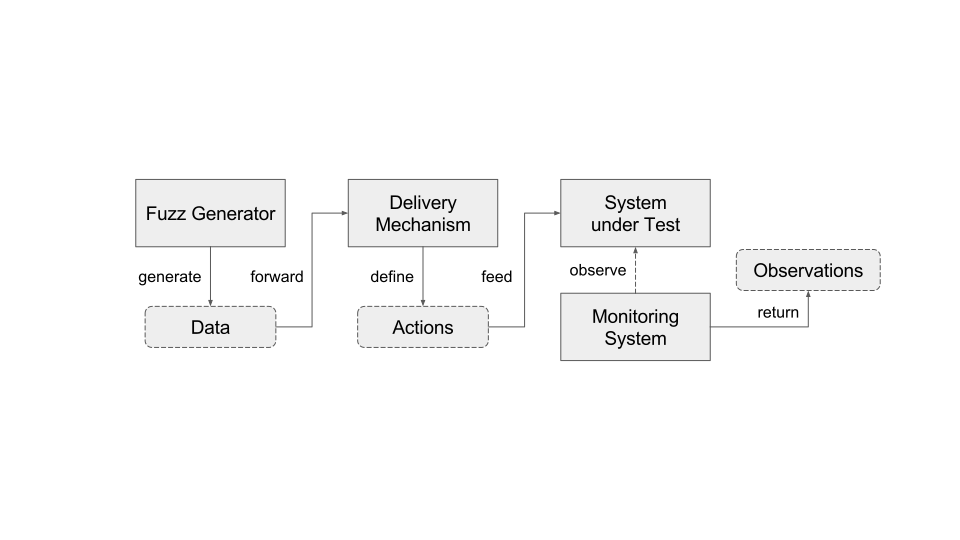
\includegraphics[width=1.0\textwidth]{images/background-fuzzing-fundamental-components.pdf}
\caption{Fundamental Components of Fuzzing}
\label{fig:backgroundFuzzingFundamentalComponents}
\end{figure}

Even though Miller et al.~showed in~\cite{miller1995fuzz} that the generation of random bytes as inputs for programs can harvest good results, its effectiveness gets limited by every conditional branch of the program under test. Each check and verification of a program requires the input data to be more structured for reaching deeper program areas. To overcome this issue two types of approaches are used by more advanced fuzz generators~\cite{takanen2008fuzzing}: \emph{mutation}-based and \emph{generation}-based techniques.

\subsection{Mutation-based fuzzing}
\label{subsec:mutatinFuzzing}

\emph{Mutation-based fuzzers}, or mutative fuzzers, take existing data and simply change it according to different rules. Such rules can be as simple as randomly toggling bits or as complex as combining two different sets of data into a new set. The advantage of mutation-based fuzzers is that they can work without the knowledge of how data must be structured and can therefore be implemented independently of the system under test. However, since they only adapt existing data, it is highly unlikely that program areas that are not bound to the existing data are exercised with the mutated data. Additionally, the advantage of using existing structured data is thwarted since the applied changes make the resulting data again more likely to be invalidated by existing checks and verifications of the program.

\subsection{Generation-based fuzzing}
\label{subsec:generationFuzzing}

\emph{Generation-based fuzzers}, or generative fuzzers, create new data without the need for existing data. They overcome the issues of mutation-based fuzzers by possessing an almost or even complete knowledge of the structure for the data that is valid for the system under test. By using this knowledge, which is called a model, data can be generated that exercises greater program coverage, since it complies to the expected structure and semantics of the system under test~\cite{miller2007analysis}.

Given that generative fuzzers have the knowledge of how valid data for a system under test has to be generated, they can be used as an efficient technique for positive testing. Hence, testing the system under test for expected behavior which includes valid as well as invalid data to test for expected error handling that is included in the specification. However, the knowledge of how valid data must be generated can also be used to derive invalid data by systematically adapting the underlying model to effectively apply negative testing. Hence, testing invalid cases which are not covered by the specification in order to provoke unexpected behavior such as system crashes.

Since one of the main goals of this thesis is to combine fuzzing and delta-debugging using the same underlying model, generative fuzzing seems to be the only logical choice for choosing an approach to implement fuzzing. However, generative fuzzing also has strong advantages over mutation-based fuzzing, such as not requiring to accumulate seemingly interesting test data, which can be a time-consuming task. Furthermore, generative fuzzing allows to accurately generate test data for specific scenarios while mutation-based fuzzing either requires to find such cases by chance or manually. An implementation of the generative fuzzing approach of this thesis can be found in Section~\ref{sec:fuzzingStrategies}. However, techniques rooted in mutation-based fuzzing can be applied to data models, thereby allowing effective negative testing in combination with mutation-based fuzzing. This exact combination has been implemented for this thesis and is described in Section~\ref{sec:fuzzingFilters}.

Even though fuzzing allows to effectively generate test data, it has the disadvantage of skipping one important part of testing software: verifying that specified requirements are implemented. In the subsequent section the software testing technique \emph{model-based testing} is introduced, which is able to fill this gap by requiring the validation of the system's output after feeding the system generated test data.

\section{What Is Model-Based Testing?}
\label{sec:whatIsModelBasedTesting}

\emph{Model-based testing} is a software testing technique which derives tests from a model that is based on the requirements on the system under tests. It is therefore a form of black-box testing. Furthermore, Utting et al.~define in \cite{utting2010practical} model-based testing to be \enquote{the automation of the design of black-box tests}, i.e., model-based testing does not only produce the input data for the execution of the system under test, but it must also generate executable test cases that include checks for the output of the system under test. An extensive list of case studies and references has been gathered by Utting et al.~in \cite{utting2010practical}, which showcase various benefits of model-based testing. Among them are reduced testing cost and time, as well as improved test quality, i.e., higher coverage of requirements testing.

The fundamental components of a model-based tester, according to~\cite{utting2010practical}, are the \texttt{Test Case Generator}, the \texttt{Test Script Generator} and the \texttt{Test Execution Tool}. These components, as well as their typical interactions, are depicted in Figure~\ref{fig:backgroundModelBasedTestingFundamentalComponents}. The test case generator uses the model to generate test cases for the system under test. These test cases may directly be executed. However, their form should be abstract in order to be able to reuse them in different environments. The test script generator then takes these test cases and transform them into test scripts which are either directly executable on the system under test, which is called online testing, or applicable using the test execution tool, which is called offline testing. The application of these test scripts outputs the final test results, i.e., whether a test case has passed the execution on the system under test.

\begin{figure}[t]
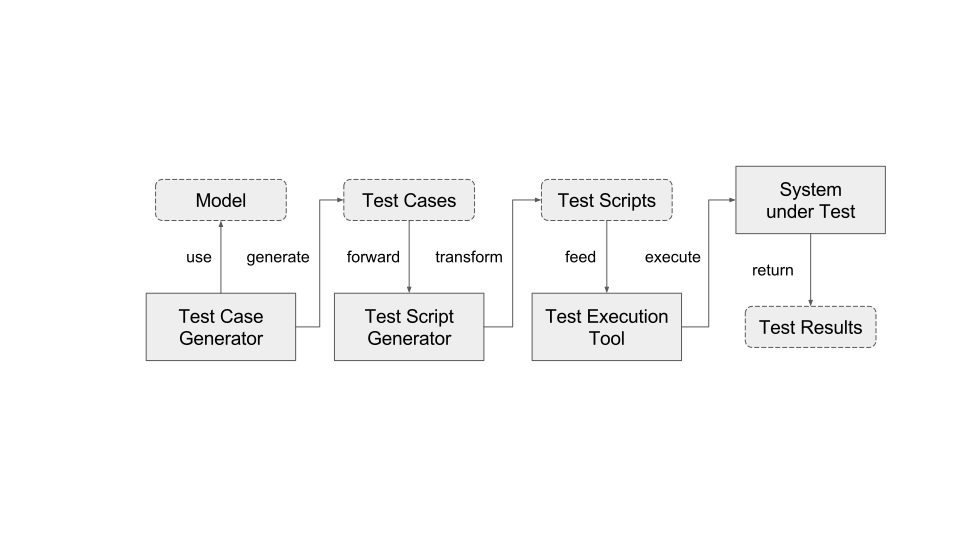
\includegraphics[width=1.0\textwidth]{images/background-modelbasedtesting-fundamental-components.pdf}
\caption{Fundamental Components of Model-based Testing}
\label{fig:backgroundModelBasedTestingFundamentalComponents}
\end{figure}

Model-based testing and generation-based fuzzing, as introduced in Section~\ref{sec:whatIsFuzzing}, utilize a data model to be able to derive and execute tests. Hence, it is only fitting to compare both techniques:
\begin{itemize}
\item The fuzz generator of the fuzzer has the same behaviors and responsibilities as the model and test case generator of a model-based tester.
\item The delivery mechanism of the fuzzer has the same behaviors and responsibilities as the test script generator and the test execution tool of the model-based tester.
\item The online testing variant of model-based testing can also be directly compared to feedback-driven fuzzing. Both techniques executed their cases directly on the system and require some kind of monitoring of the system under test. The feedback of the monitoring can then be incorporated into the test cases, e.g., to check if an error message occurred, and guide the generation of the next test case.
\end{itemize}
Even though we can directly compare generation-based fuzzing to model-based testing, we can also observe three major differences: Model-based testing is much stricter concerning the model which is used to generate test cases. It has to be based on the requirements of the system under test. Furthermore, the validation of the system's output, which is a requirement for model-based testing, is not necessary for a fuzzer, but can be adopted by the monitoring system. Lastly, model-based testing strives to generate reusable test cases which are semi-executable, while fuzzing is often described of only generating inputs which can be used as parameters for test cases or the execution of the system under test.

These differences make model-based testing an attractive addition to fuzzing to completely cover the whole spectrum of software testing. As a result, this thesis introduces with the \textsc{Tavor framework} in Chapter~\ref{chapter:tavorFramework} and the \textsc{Tavor format} in Chapter~\ref{chapter:tavorFormat} capabilities to define and structure functional test cases which include the validation of requirements. Furthermore, Chapter~\ref{chapter:tavorCLI} introduces with the \textsc{Tavor CLI} functionality to communicate with the systems under test. These additions allow the utilization of model-based testing which are showcased in the evaluation presented in Chapter~\ref{chapter:evaluation}.

Since both, fuzzing and model-based testing, allow to generate test cases to form test suites, a suitable method for evaluating these test suites must be employed. The subsequent section introduces \emph{mutation testing}, which allows to measure the effectiveness of a test suite to detect faults in the system under test.

\section{What Is Mutation Testing?}
\label{sec:whatIsMutatinTesting}

\emph{Mutation testing} is, according to an extensive survey by Jia et al.~\cite{jia2011analysis}, a \enquote{fault-based testing technique which can be used to measure the effectiveness of a test set in terms of its ability to detect faults}. The technique introduces faults, which are represented as syntactical changes to the program's binary or source code called \emph{mutations}, to create faulty programs named \emph{mutants}. Each mutant is then tested by executing an existing test set of the program. If the result of running the test set with the mutant differs from the result of running the test set with the original fault-free program, then the mutant has been killed, i.e., it has been detected by the test set. If the mutant has not been killed, either the test set needs to be extended to detect the modification or the mutant is equal to the original program. The effectiveness of the test set can then be calculated by the number of killed mutants by the total amount of tested mutants. This metric is called the \emph{mutation score} which can be used to directly compare two distinct test sets for the same program. Hence it can, for instance, be used to compare handwritten to automatically generated test sets of programs. A mutation score of $1.0$ is most desirable since this means that a test set killed all mutations.

Significant to the field of mutation testing are two hypothesis defined by DeMillo et al.~\cite{demillo1978hints}: the \emph{Competent Programmer Hypothesis} and the \emph{Coupling Effect}. They imply that it should be sufficient to examine only a subset of simple faults of the overall possible program faults, to be effective in finding real faults~\cite{jia2011analysis}.
\begin{itemize}
\item The \emph{Competent Programmer Hypothesis} states that \enquote{programmers are competent, which implies that they tend to develop programs close to the correct version}~\cite{jia2011analysis}. It can be therefore assumed that the existing faults in a program are simple. Therefore, it is sufficient to introduce simple faults by mutation testing because it mimics the faults that are made by competent programmers.
\item The \emph{Coupling Effect} states that \enquote{test data that distinguishes all programs differing from a correct one by only simple errors is so sensitive that it also implicitly distinguishes more complex errors} \cite{demillo1978hints}. Therefore, it is sufficient to examine only simple errors since they are coupled with complex errors in the program under test.
\end{itemize}

The fundamental components of mutation testing can be derived from the traditional process described in~\cite{demillo1978hints, jia2011analysis}, namely: the list of \texttt{Mutation Operators} to apply modifications and a \texttt{Test Set} of the program under test. These components, as well as their typical interactions, are depicted in Figure~\ref{fig:backgroundMutationTestingFundamentalComponents}. First the original program $P$ is executed against the test set $T$, producing the test result $R$. Then each mutation operator $M$ takes the original program under test $P$ and applies its modifications. The outcome is a set of modified programs $P'$, the so called mutants. These modified programs $P'$ are then executed against the test set $T$. The produced test results $R'$ of this step are compared to the original test result $R$. If the results are equal, the mutant $P'$, and therefore its modifications, has not been detected by the test set $T$.

\begin{figure}[t]
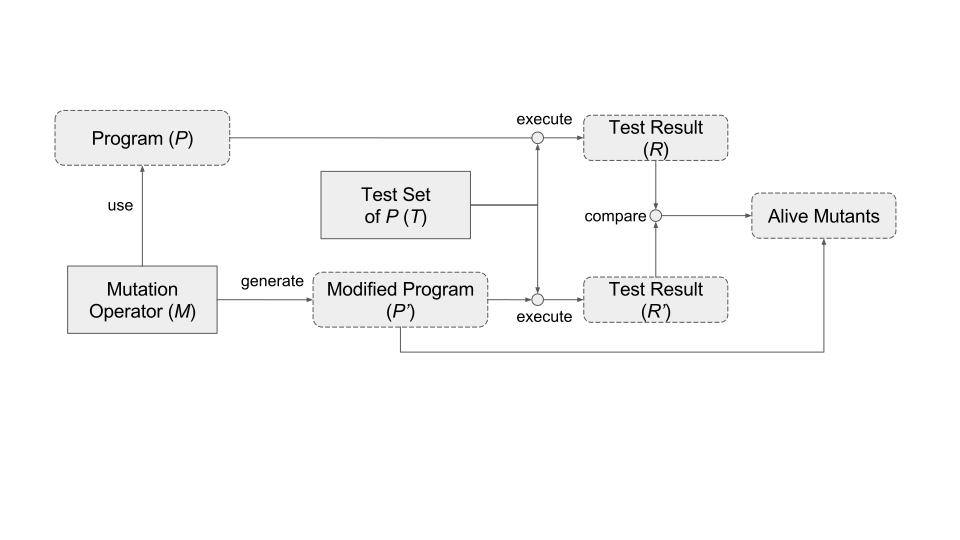
\includegraphics[width=1.0\textwidth]{images/background-mutationtesting-fundamental-components.pdf}
\caption{Fundamental Components of Mutation Testing}
\label{fig:backgroundMutationTestingFundamentalComponents}
\end{figure}

Although the definition of mutation testing states that it is applied to detect faults in programs, it can also be used to uncover implementation flaws such as dead code. Furthermore, mutation testing is mostly described to solely cover techniques for program source code. However, it has also been used to mutate program specifications~\cite{jia2011analysis}. The latter direction is called \emph{specification mutation}, which is a black-box or grey-box testing technique depending on what program parts are used, while the first direction is called \emph{program mutation} which solely focuses on the program binary or source code and is therefore a white-box testing technique~\cite{jia2011analysis}.

This thesis utilizes mutation testing in Chapter~\ref{chapter:evaluation} to evaluate the effectiveness of generated test suites. The direction of program mutation is used, to emphasize how much of the system under test is actually covered. Since everything that has been implemented for this thesis is written in the programming language \textsc{Go}, it is only fitting to include in the evaluation of this thesis at least one scenario of a \textsc{Go} program. Chapter~\ref{chapter:goMutesting} introduces \textsc{go-mutesting} to perform the mutation testing part for the evaluation of the mentioned scenario.

Determining the effectiveness of test suites is just one discipline that needs to be considered while generating test cases. Another discipline arises when individual test cases are executed. The execution of a test case either verifies that the system under test behaves as defined by the test case, or the test case fails which highlights a fault that must be investigated. One possible method to aid in the time-consuming and complicated process of investigating and patching faults is the reduction of failing test cases. The subsequent section introduces \emph{delta-debugging}, an automatic technique to systematically reduce data such as test cases.

\section{What Is Delta-Debugging?}
\label{sec:whatIsDeltaDebugging}

\emph{Delta-debugging} is defined by Zeller in~\cite{zeller2009programs} as an \enquote{automatic technique that narrows down a cause by running automated experiments}. The typical use case is the reduction of input data which lets a program fail during execution. Less data has the benefit of having to consider less context during debugging a problem. Therefore, delta-debugging makes it possible for the user to focus only on relevant parts of the failure-inducing data. Note that finding the minimal representation, which still provokes the same program behavior of the original data, is not guaranteed by process of delta-debugging~\cite{brummayer2009fuzzing, brummayer2010automated}. However, in practice every reduction of the context that is needed to debug a problem is already an improvement. Furthermore, delta-debugging can be used to reduce and isolate anything, given appropriate implementations of the delta-debugging phases. For instance a solution might be reduced to be more readable or a huge formula is rewritten to a smaller formula which has the same behavior.

The fundamental components of a delta-debugger, which can be derived from the original algorithm~\cite{zeller2009programs}, are the \texttt{Reduction Algorithm} and the \texttt{System Under Test}. These components, as well as their typical interactions, are depicted in Figure~\ref{fig:backgroundDeltaDebuggingFundamentalComponents}. First the original data $D$ is executed with the system under test. The resulting execution determines the original behavior $B$ which must be preserved during the reduction. Next the original data $D$ is fed into the reduction algorithm. The algorithm determines which parts of the data should be reduced for the current reduction iteration, and how the selected part is reduced, i.e., removed or substituted. The reduced data $D'$ is then executed with the system under test. The resulting behavior of the execution $B'$ is compared to the behavior of the execution with the original data $B$. The result of this comparison is fed back into the reduction algorithm. If both behaviors are the same, the original behavior got preserved and the reduction algorithm continues with the next reduction iteration. Otherwise the last reduction is reverted and the algorithm proceeds. This reduction loop continues until predefined conditions are met, e.g., a timeout occurs or the algorithm does not find new parts to reduce.

\begin{figure}[t]
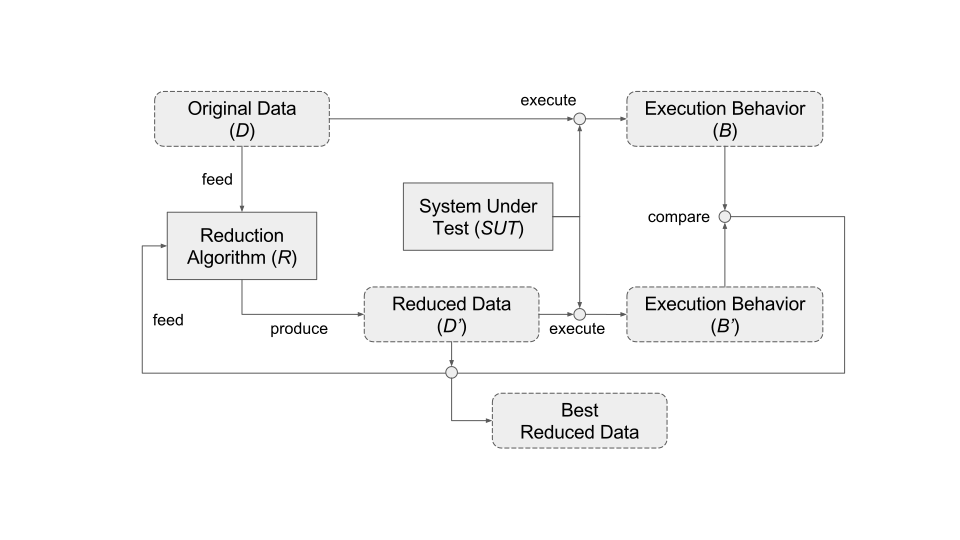
\includegraphics[width=1.0\textwidth]{images/background-deltadebugging-fundamental-components.pdf}
\caption{Fundamental Components of Delta-Debugging}
\label{fig:backgroundDeltaDebuggingFundamentalComponents}
\end{figure}

Considering the main components and workflow of delta-debugging, we can define the following three phases:

\begin{itemize}
\item The \emph{search phase} decides which part of the data will be reduced next.
\item The \emph{reduction phase} removes repetitions and optional data or replaces data with something else, e.g., uninteresting complex functions are replaced with constant values.
\item The \emph{testing phase} checks if the reduced data still provokes the original failure.
\end{itemize}

The original delta-debugging algorithm~\cite{zeller2009programs} reduces the given data at the character level, ignoring the syntactical structure of the data. Hence, making it likely to produce invalid data, leading to a high amount of rejected reduction iterations. By making the search phase aware of the data's structure an immense reduction in iterations can be achieved, dramatically speeding up the delta-debugging process~\cite{misherghi2006hdd, brummayer2009fuzzing, brummayer2010automated}. Additionally, making the reduction phase aware of the content itself, can be very efficient in reducing the original data greatly while also reducing the runtime of the process~\cite{brummayer2009fuzzing, brummayer2010automated}.

Making the delta-debugging implementation aware of the data's structure and content, basically giving the implementation an almost or even complete model of the provided data, is one of the goals of this thesis. Section~\ref{sec:reducingStrategies} describes the approach and implementation which completes the goal of combining fuzzing and delta-debugging by utilizing the same underlying model.

\chapter{The \textsc{Tavor Framework}}
\label{chapter:tavorFramework}

The main goal of \textsc{Tavor} is to provide functionality for the automatic generation, alteration and reduction of test data which conforms to a predefined structure. Programs oftentimes need to process complex data structures that allow for an enormous number of possible variants. Such programs are therefore hard to test, since a tester has to consider every important variant for testing purposes. To construct the input data manually is time-intensive and error-prone. \textsc{Tavor} can be used to automate the generation of this data, to alter existing data and to apply delta-debugging to systematically reduce existing data according to a predefined structure and its constraints.

\begin{figure}[hb]
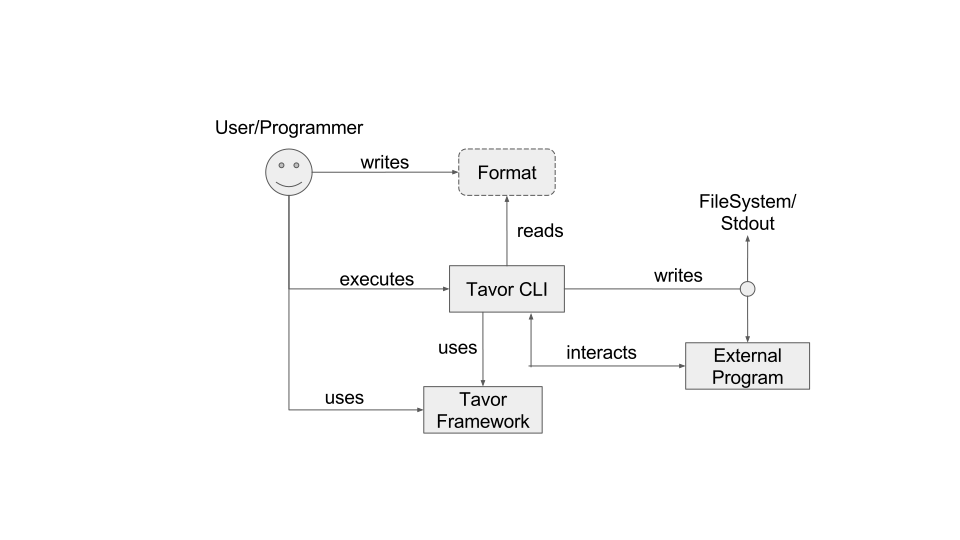
\includegraphics[width=0.8\textwidth]{images/tavor-interactions.pdf}
\caption{\textsc{Tavor}'s subsystems}
\label{fig:tavor-interactions}
\end{figure}

Figure~\ref{fig:tavor-interactions} depicts the interactions of the \textsc{Tavor} subsystems. In order to interact with an external program a user first needs to define a data model which describes the structure of the expected inputs to the program. The \textsc{Tavor framework} provides its own format to define such data models, which covers all functionality of the framework. Please refer to Chapter~\ref{chapter:tavorFormat} for a detailed description of the \textsc{Tavor format} and its capabilities. Next, the \textsc{Tavor CLI} can be used to interact with an external program. Interactions such as fuzzing or delta-debugging are also provided by the \textsc{Tavor CLI}, which is described in more detail in Chapter~\ref{chapter:tavorFormat}. The \textsc{Tavor CLI} relies heavily on the algorithms and data structures provided by the \textsc{Tavor framework}. The framework's design goals as well as its components and their interactions are the main focus of the subsequent sections of this chapter.

\section{Components}
\label{sec:components}

The \textsc{Tavor framework} offers various components which are depicted in Figure~\ref{fig:tavor-components}. There are three utility components, i.e., \texttt{Tokens}, \texttt{Parsers} and \texttt{Logging}, as well as three components offering access to different kinds of algorithms, i.e., \texttt{Fuzzing Strategies}, \texttt{Fuzzing Filters} and \texttt{Reducing Strategies}.

\begin{figure}[ht]
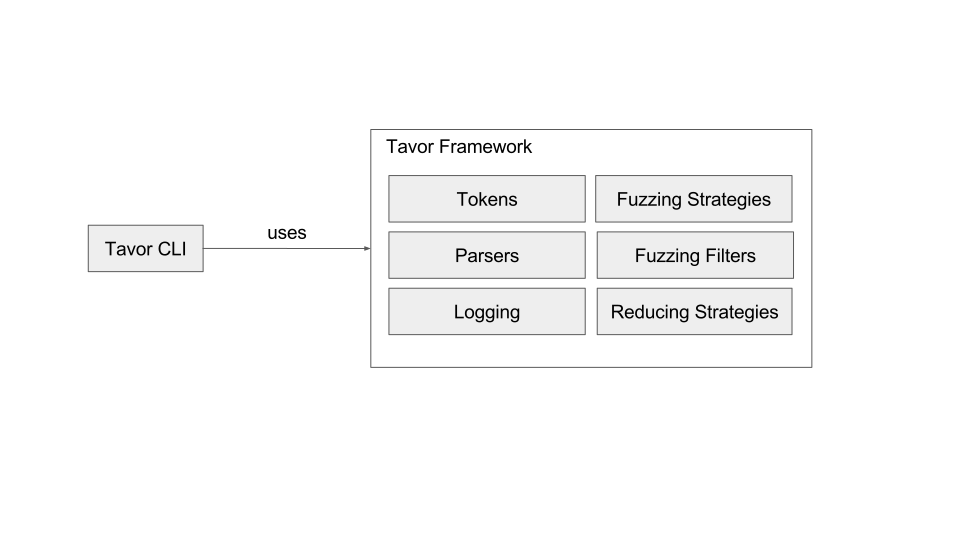
\includegraphics[width=1.0\textwidth]{images/tavor-components.pdf}
\caption{Components of the \textsc{Tavor framework}}
\label{fig:tavor-components}
\end{figure}

In order to combine both, fuzzing and delta-debugging, all implemented methods of the \textsc{Tavor framework} operate on one internal model-based structure. This structure is basically a graph of nodes that are called \texttt{token graphs} throughout the \textsc{Tavor framework}. Each node represents an instance of a \texttt{token} of a framework-defined type. A token graph can either be directly instantiated or by parsing a format file using the \texttt{Parsers} component of the \textsc{Tavor framework}. The \texttt{Logging} component provides extensive logging for debugging the handling of tokens. The granularity of logged output can be controlled by specifying the desired log level, i.e., the debug level reports the widest range of information while the error level only informs about occurred errors.

Instead of focusing on only one technique \textsc{Tavor}'s components have been kept generic. Dedicated techniques and heuristics can be implemented and executed independently. All of these components operate on tokens. In order to generate permutations of a specific token, i.e., unique arrangements of the token's values, \texttt{fuzzing strategies} are used. A token itself is not fixed to a static definition but can be changed by \texttt{fuzzing filters} to apply additional techniques such as boundary-value analysis of ranges. For delta-debugging so called \texttt{reducing strategies} can be implemented and used.

Every algorithm of the \textsc{Tavor framework} has to be deterministic, since determinism has the advantage that it eases debugging problems and enables the reproduction of results that are sent to external programs. Therefore, no functionality is allowed to have its own source or seed of randomness. Instead, a common interface that defines a random generator is used throughout the framework. An implementation of this interface has to be deterministic given the same seed of randomness. The decision of keeping code deterministic was also applied to concurrent code and tests, making it possible to reproduce the same output given the same random seed and version of the framework.

The following subsections present \textsc{Tavor}'s fundamental implementation decision as well as its main components \texttt{Tokens}, \texttt{Fuzzing Strategies}, \texttt{Fuzzing Filters} and \texttt{Reducing Strategies} in more detail.

\section{Tokens}
\label{sec:tokens}

The basic building blocks of the \textsc{Tavor framework} are its \emph{tokens}. These tokens differ from \emph{lexical analysis tokens} in the following way: They represent not just a group of characters, but different kinds of data with additional properties and abilities. Tokens can be constant integers and strings of all kind as well as dynamic data such as integer ranges, sequences and character classes. Furthermore, tokens can encapsulate other tokens to group them together and to create building blocks that can be reused to, for example, repeat a group of tokens. Tokens can have states, conditions and can perform operations such as arithmetic. They can create new tokens dynamically and can depend on other tokens to generate data. Tokens are basically the foundation of the framework and every algorithm for parsing, fuzzing and delta-debugging is relying on them.

A \emph{permutation} of a token is a specific arrangement of its values. Every token type has its own arrangement implementation and every token instance can have its own values. However, the set of permutations is unique for a specific token type and values, as is the order of these permutations. For example a token holding a range of numbers from \enquote{4} to \enquote{6} has 3 possible permutations: \enquote{4}, \enquote{5} and \enquote{6}. The first permutation of this token is \enquote{4} and the third permutation is \enquote{6}. Even though this demonstrates that a token can represent many permutations, every token can hold only one permutation at any given time. Therefore, every token implementation should differentiate between an internal and external representation. Since it is necessary to save the possible values internally but to forward the current value externally. This distinction is especially important for token types that generate new tokens out of their internal representation. The original internal tokens should not be connected to the external ones, since it would be otherwise possible to change the internal representation without any contract.

Many of the algorithms in the \textsc{Tavor framework} build upon the assumption that the processed token graphs are acyclic. This decision allows for easier implementations and usage since no guards and functionality have to implemented to deal with infinitely running algorithms and unwanted repetitions. Hence, while the internal structure allows tokens to have loops in their graphs, each loop must be unrolled before it can be used with the algorithms of the \textsc{Tavor framework}, i.e., the bodies of repetitions are copied N-times instead of the original repetition. An example for a token graph with a loop is given in Figure~\ref{fig:unroll-loop} which is then unrolled twice resulting in the graph of Figure~\ref{fig:unroll-unrolled}.

\begin{figure}[ht]
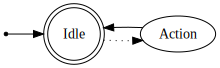
\includegraphics[height=0.125\textwidth]{images/unroll-loop.pdf}
\caption{Example for a Graph with a Loop}
\label{fig:unroll-loop}
\end{figure}

\begin{figure}[ht]
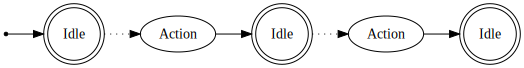
\includegraphics[height=0.1\textwidth]{images/unroll-unrolled.pdf}
\caption{Example for an Unrolled Graph}
\label{fig:unroll-unrolled}
\end{figure}

Every token implements at least the basic \emph{Token Interface}, which specifies methods for generating, replicating, permutating and parsing. Additional token interfaces add specific functionality to a token. The \emph{List Interface}, for example, states that a token can have child tokens and specifies methods to access them.

The Token Interface is the base interface of all tokens. Its operations can be grouped into the following categories:

\begin{itemize}
\item \textit{Generation} to output the external representation of the token.
\item \textit{Replication} to create an exact copy of the token.
\item \textit{Permutation} to permutate the token.
\item \textit{Parsing} to parse arbitrary input to permutate the token.
\end{itemize}

Subsection~\ref{subsec:tokens-smiley} presents an example token implementation which exemplifies the above-mentioned fundamental token concepts. Subsequently Subsection~\ref{subsec:tokens-advanced-concepts} elaborates on advanced token concepts, which are for instance necessary to model repetitions or constraints.

\subsection{Example Implementation - The \textsc{Smiley} Token}
\label{subsec:tokens-smiley}

This subsection illustrates the implementation of a basic \textsc{Tavor} Token, thus explaining the fundamental token operations by example. Since the \textsc{Tavor framework} is written in the programming language \textsc{Go}, the following implementations are written in \textsc{Go} as well. \textsc{Go} is an open source programming language created at Google. The language is garbage collected which allows the following examples to be nearly uncluttered of memory handling. Furthermore, \textsc{Go}'s C-like syntax should be widely readable with the exceptions of three operators: The \emph{short variable declaration} operator \enquote{:=} declares and initializes a variable using the value and variable type of the right-hand side of the operator. The range operator allows the programmer to iterate over an array using a for-loop, e.g., \texttt{for i, p := range people} iterates over the variable \texttt{people} with \texttt{i} holding the index and \texttt{p} holding the item of the current iteration. Lastly, the \enquote{go} operator starts the encapsulated function call in a new coroutine.

Consider a token defining a smiley which has eyes, a mouth and can have a nose. The token should be able to generate different permutations of smilies and even parse them. This example uses two different kinds of eyes: \enquote{\texttt{:}} and \enquote{\texttt{;}}, an optional nose \enquote{\texttt{-}} and three different kinds of mouths: \enquote{\texttt{)}}, \enquote{\texttt{(}} and \enquote{\texttt{D}}. Thus, we allow for instance the smiley \enquote{\texttt{;-D}}, but not \enquote{\texttt{:-<}}. This example should in general show how easy it is to create new token types. It must be noted that this example could be easily implemented with the available token types or with the \textsc{Tavor format} shown in Listing~\ref{lst:smiley-format}.

\begin{listing}
\caption{Smiley \textsc{Tavor format}}
\label{lst:smiley-format}
\begin{gocode}
START = [:;] ?("-") [)(D]
\end{gocode}
\end{listing}

Listing~\ref{lst:smiley-data-structure} shows the basic data structure of the \textsc{Smiley} Token. Since the \textsc{Smiley} Token has to hold three different types of information, it is necessary to create a structure. Instead of directly using the characters for the eyes and mouth in the structure, only indices are used. This is not necessary but helps to separate the constant data from the permutation of the token. Using this data structure the smiley \enquote{\texttt{;-D}} would be represented with the composite literal \texttt{Smiley\string{eyes:~1, nose:~true, mouth:~2\string}}. The structure must implement the Token Interface, which is grouped into method categories as described in Section~\ref{sec:tokens}. The implementations of these categories are now presented in the remainder of this section.

\begin{listing}
\caption{Smiley Data Structure}
\label{lst:smiley-data-structure}
\begin{gocode}
var (
	eyes   = ":;"
	mouths = ")(D"
)

type Smiley struct {
	eyes  int
	nose  bool
	mouth int
}
\end{gocode}
\end{listing}

The \textit{Generation} category of the Token Interface deals with the output of the current permutation. To implement this category at least the \texttt{String} method has to be implemented, which returns the textual representation of the token's current permutation. The \texttt{String} method for the \textsc{Smiley} Token is shown in Listing~\ref{lst:smiley-string-method}, and returns for the smiley \texttt{Smiley\string{eyes:~1, nose:~true, mouth:~2\string}} the string \enquote{\texttt{;-D}}. Since the internal representation should not be accessible by the token's user, no safeguards, e.g., for accessing array items by their indices, are necessary.

\begin{listing}
\caption{Smiley \texttt{String} Method}
\label{lst:smiley-string-method}
\begin{gocode}
func (s *Smiley) String() string {
	nose := ""
	if s.nose {
		nose = "-"
	}

	return string(eyes[s.eyes]) + nose + string(mouths[s.mouth])
}
\end{gocode}
\end{listing}

The \textit{Replication} category deals with replicating tokens, i.e., with creating copies of tokens. The \texttt{Clone} method is the only replication function required by the Token Interface. Note that the new token must be independent of the original token, i.e., that each \texttt{Clone} function needs to perform a deep rather than a shallow copy of its data. For the \textsc{Go} programming language this means that token internal slices, maps, structures and token children must be copied as well. The implementation of the \texttt{Clone} method for the \textsc{Smiley} Token is shown in Listing~\ref{lst:smiley-clone-method}.

\begin{listing}
\caption{Smiley \texttt{Clone} Method}
\label{lst:smiley-clone-method}
\begin{gocode}
func (s *Smiley) Clone() token.Token {
	return &Smiley{
		eyes:  s.eyes,
		nose:  s.nose,
		mouth: s.mouth,
	}
}
\end{gocode}
\end{listing}

The \textit{Permutation} category handles the set of permutations for a token as well as its current permutation. The method \texttt{Permutations} defines how many permutations a single token holds. The \textsc{Smiley} Token has a constant number of 12 permutations, since the amount of eyes, mouths and noses is constant. Other tokens such as ranges of integers depend on their configuration. The implementation of the \texttt{Permutations} method for the \textsc{Smiley} Token is shown in Listing~\ref{lst:smiley-permutations-method}.

\begin{listing}
\caption{Smiley \texttt{Permutations} Method}
\label{lst:smiley-permutations-method}
\begin{gocode}
func (s *Smiley) Permutations() uint {
	return uint(len(eyes) * 2 * len(mouths))
}
\end{gocode}
\end{listing}

The method \texttt{PermutationsAll} returns the number of permutations of the token itself and all its children. Since the \textsc{Smiley} Token has no children, it is the same as \texttt{Permutations} which is shown in Listing~\ref{lst:smiley-permutationsAll-method}. However, it is important to note that calculating the amount of permutations is not always a straightforward task. Consider for instance the \emph{Concatenation Token} representing a sequence of tokens, which requires all of its children to be present, and the \emph{One Token}, which requires exactly one of its children to be present. These two tokens have very different permutation calculations. For the Concatenation Token the product of its children's \texttt{PermutationsAll} result is calculated using $\prod_{i=1}^{token. NumChildren} Token.Child(i).PermutationsAll()$ while for the One Token the sum of its children's \texttt{PermutationsAll} result is calculated using $\sum_{i=1}^{token. NumChildren} Token.Child(i).PermutationsAll()$.

\begin{listing}
\caption{Smiley \texttt{PermutationsAll} Method}
\label{lst:smiley-permutationsAll-method}
\begin{gocode}
func (s *Smiley) PermutationsAll() uint {
	return s.Permutations()
}
\end{gocode}
\end{listing}

The \texttt{Permutation} method completes the \textit{Permutation} category. It sets a distinct permutation of the token, i.e., calling the method with the integer 11 results in \texttt{Smiley\string{eyes:~1, nose:~true, mouth:~2\string}} which represents the \texttt{;-D} smiley. The implementation of the \texttt{Permutation} method for the \textsc{Smiley} Token is shown in Listing~\ref{lst:smiley-permutation-method}, and has been intentionally been made inefficiently to keep the example simple.

\begin{listing}
\caption{Smiley \texttt{Permutation} Method}
\label{lst:smiley-permutation-method}
\begin{gocode}
func (s *Smiley) Permutation(i uint) error {
	if i < 0 || i >= s.Permutations() {
		return NewPermutationErrorIndexOutOfBound()
	}

	p := uint(0)
	for eyes := range eyes {
		for _, nose := range []bool{false, true} {
			for mouth := range mouths {
				if i == p {
					s.eyes = eyes
					s.nose = nose
					s.mouth = mouth

					return nil
				}

				p++
			}
		}
	}

	return nil
}
\end{gocode}
\end{listing}

Finally, the \texttt{Parsing} category, which is the last category of the Token Interface, deals with parsing the token from an input. Listing~\ref{lst:smiley-parse-method} shows the \texttt{Parse} method of the \textsc{Smiley} Token. The implementation may look very verbose, but it is necessary to handle every syntax error to generate adequate parsing errors. Note that these messages could be further improved by not only stating that something was expected, but actually giving examples on what has been expected.

\begin{listing}
\caption{Smiley \texttt{Parse} Method}
\label{lst:smiley-parse-method}
\begin{gocode}
func (s *Smiley) Parse(parser InternalParser, cur int) (int, []error) {
	if cur+2 > parser.DataLen {
		return cur, []error{errors.New("Out of data for a smiley")}
	}

	if i := strings.IndexRune(eyes, parser.Data[cur]); i != -1 {
		s.eyes = i
	} else {
		return cur, []error{errors.New("Expected some eyes")}
	}
	cur++

	if parser.Data[cur] == '-' {
		s.nose = true
		cur++
	} else {
		s.nose = false
	}
	if cur >= parser.DataLen {
		return cur, []error{errors.New("Out of data for a mouth")}
	}

	if i := strings.IndexRune(mouths, parser.Data[cur]); i != -1 {
		s.mouth = i
	} else {
		return cur, []error{errors.New("Expected a mouth")}
	}
	cur++

	return cur, nil
}
\end{gocode}
\end{listing}

The \textsc{Smiley} Token can then be used to create structures like with any other token of the framework. However, to give an easier example, it will be used alone. Listing~\ref{lst:working-with-smiley} creates a new \textsc{Smiley} Token, permutates over all permutations and parses a string. Each step is printed to STDOUT. Resulting in the output shown in Listing~\ref{lst:working-with-smiley-output}.

Please note, that the smiley token has been used to demonstrate, which standard methods each token type needs to implement. Of course, the \textsc{Tavor framework} already offers a wide range of token types allowing to represent arbitrary formats. Chapter~\ref{chapter:tavorFormat} gives an overview of the format options that are already implemented by the tokens of the \textsc{Tavor framework}.

\begin{listing}
\caption{Working with the \textsc{Smiley} Token}
\label{lst:working-with-smiley}
\begin{gocode}
func main() {
	s := Smiley{}

	fmt.Print("Permutations:")
	for i := uint(0); i < s.Permutations(); i++ {
		s.Permutation(i)
		fmt.Print(" ", s.String())
	}
	fmt.Println()

	p := NewInternalParser(":-D")
	_, errs := s.Parse(p, 0)
	if errs != nil {
		panic(errs)
	}

	fmt.Println("Parsed:", s.String())
}
\end{gocode}
\end{listing}

\begin{listing}
\caption{Output of Smiley Example}
\label{lst:working-with-smiley-output}
\begin{textcode}
Permutations: :) :( :D :-) :-( :-D ;) ;( ;D ;-) ;-( ;-D
Parsed: :-D
\end{textcode}
\end{listing}

\subsection{Advanced Token Concepts}
\label{subsec:tokens-advanced-concepts}

While \textsc{Tavor} actually lacks the \textsc{Smiley} Token introduced in Subsection~\ref{subsec:tokens-smiley}, it offers a wide range of different token types, which can be used to model arbitrary formats.
The following categories of tokens give an excerpt of the different tokens supported by \textsc{Tavor}:

\begin{itemize}
\item \textit{Primitive} Tokens do not reference other tokens, i.e., they are vertices in the token graph without any outgoing edges. These tokens solely implement the basic Token Interface. The plainest types are the \texttt{Integer} and \texttt{String} Tokens, which represent constant data of numbers and texts, e.g., \enquote{1234} and \enquote{"Hello World}. Other examples of this category, such as the as \texttt{RangeInt} which allows to define a range of integers, are dynamic, i.e., can have more than one permutation, but can represent only one permutation at any given time. Another example is the \texttt{CharacterClass} Token, most commonly known from regular expressions, which allows to define character class definitions such as \texttt{[ACE]} allowing either one of the characters \enquote{A}, \enquote{C} or \enquote{E}.
\item \textit{List} Tokens contain a list of child tokens. Additionally to the basic Token Interface these tokens also implement the List Interface, which provides methods to operate on the token's children. At the moment of writing the token types \texttt{Concatenation}, \texttt{Once}, \texttt{One} and \texttt{Repeat} are currently supported. The \texttt{Concatenation} (resp. \texttt{Once}) Token requires all children to be present in the defined order (resp. an arbitrary order). The \texttt{One} Token allows to define lists were exactly one child token is present in every permutation. Finally the \texttt{Repeat} Token is used to repeat defined tokens for a specified amount of times.
\item \textit{Constraint} Tokens are used to bind tokens to constraints, e.g., the \texttt{Optional} Token expresses that the wrapped token may or may not be present.
\item \textit{Expression} Tokens are used to define formulas, consisting of one or more token, which can be resolved to a single value, which is again a token. Such tokens can be for example arithmetically such as \texttt{ArithmeticAdd}, \texttt{ArithmeticSub}, \texttt{ArithmeticMul} and \texttt{ArithmeticDiv} which allow simple calculations of numbers. The \texttt{BooleanTrue} and \texttt{BooleanEqual} are another example of expression tokens, which belong to the scope of boolean algebra.
\item \textit{Statement} Tokens are used to handle control flows in token graphs, e.g., the \texttt{If} Token uses a boolean expression to guard a child token which is only active if the expression is true.
\item \textit{Variable} Tokens have been implemented in order to be able to reuse and interact with generated values at another place in a token graph.
\end{itemize}

Every token type and interface can have its own \textit{token attributes}, which are used to access meta information about a token. Each List token, for instance, provides the attributes \texttt{Count} to retrieve to the number of its child tokens, \texttt{Item(i)} to refer to its i-th child and \texttt{Unique} to refer to an arbitrary but unique child of the list.

Consider Figure~\ref{fig:automaton-simple-format}, it shows an automaton which allows an \enquote{a} character, followed by two to four \enquote{b}, an optional \enquote{c} and a concluding \enquote{d}. The token graph representing this format is shown in Figure~\ref{fig:token-graph-simple-format}. It is rooted in a \texttt{Concatenation} Token which has four child tokens. The starting and concluding tokens are simply constant strings, i.e., they need to be present in every permutation. The repetition of \enquote{b} is expressed using a \texttt{Repeat} Token with the configuration \texttt{from=2} and \texttt{to=4}. In order to model that the String Token \enquote{b} is optional it is wrapped in an \texttt{Optional} Token.

\begin{figure}
\begin{center}
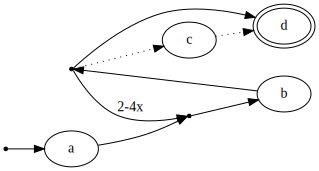
\includegraphics[height=0.3\textwidth]{images/tavor-simple-format.pdf}
\caption{Automaton of Simple Format Definition}
\label{fig:automaton-simple-format}
\end{center}
\end{figure}

\begin{figure}[ht]
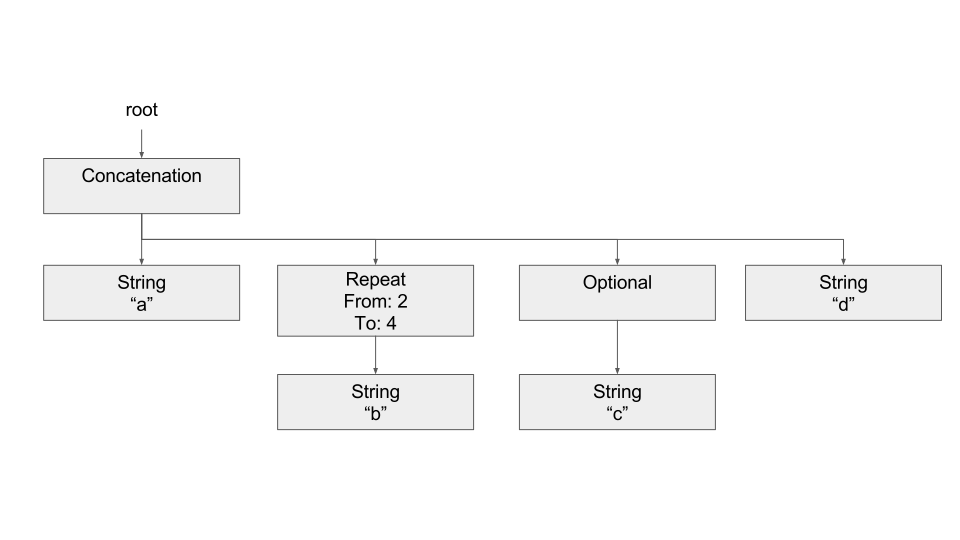
\includegraphics[width=1.0\textwidth]{images/tavor-simple-format-token-graph.pdf}
\caption{Token Graph of Simple Format Definition}
\label{fig:token-graph-simple-format}
\end{figure}

Most algorithms of the \textsc{Tavor framework} traverse a token graph and perform a certain operation on each traversed token. Auxiliary functions are provided by the framework to fulfill this purpose. One of these functions is \texttt{Walk} which is depicted as pseudo code in Listing~\ref{lst:walk-func}. It receives two input parameter: the \texttt{root} Token which needs to be traversed and the function \texttt{walkFunc} which is called for each traversed token. A queue is used to systematically traverse the token graph. Remember, no cycles are allowed within a token graph. Hence, no loop-detection needs to be implemented. Tokens that implement the Forward Interface, which reference a single token, are handled in Line~14, which pushes the referenced child for later processing onto the queue. The List Interface is implemented by those token types who refer to a list of child tokens, hence the loop from Lines~16-18 is used to add all referenced children onto the queue.

\begin{listing}
\caption{Token Graph Walk Function}
\label{lst:walk-func}
\begin{gocode}
func Walk(root Token, walkFunc func(token Token) error) error {
	queue := NewQueue()
	queue.Push(root)

	for !queue.Empty() {
		token := queue.Pop()

		if err := walkFunc(token); err != nil {
			return err
		}

		switch t := token.(type) {
		case Forward:
			queue.Push(t.Get())
		case List:
			for i := t.Len() - 1; i >= 0; i-- {
				queue.Push(t.Get(i))
			}
		}
	}

	return nil
}
\end{gocode}
\end{listing}

\section{Fuzzing Strategies}
\label{sec:fuzzingStrategies}

The \textsc{Tavor framework} provides the concept of fuzzing strategies to generate permutations of a token graph according to a specific algorithm. There are two fundamental ways of token fuzzing. One is to deterministically choose one possible permutation, the other is to choose randomly out of all permutations of a token. All fuzzing strategies need to implement the following interface:

\begin{center} \texttt{type Strategy func(root Token, r rand.Rand) (chan bool, error)} \end{center}

This interface defines a single function, which initializes the strategy and then starts the first fuzzing iteration in a new coroutine. If an error is encountered during the initialization of the strategy, the error return argument is not nil. On success a channel is returned, which controls the fuzzing process. In the \textsc{Go} programming language channels are used to communicate among coroutines. For each completed iteration of the fuzzing strategy a value is returned by the channel. The caller of the strategy needs to put back a value into the channel, to initiate the calculation of the next fuzzing iteration. This passing of values is needed to avoid data races within the token graph. Note that the channel must be closed either when there are no more iterations, or in case the caller of the strategy wants to end the fuzzing process.

The \textsc{Tavor framework} provides the following default fuzzing strategies:
\begin{itemize}
\item The \emph{Random} strategy generates exactly one permutation of the passed in token graph by permuting each reachable token randomly. The determinism is dependent on the random generator and is therefore deterministic if the same random seed is used for initializing the random generator.
\item The \emph{AllPermutations} strategy deterministically generates all available permutations of a token.
\item The \emph{AllmostAllPermutations} strategy generates a subset of all available permutations by not covering all possible permutations of Repeat Tokens. This capability is especially helpful when less permutations are needed than provided by the \emph{AllPermutations} strategy.
\item The \emph{PermuteOptionals} strategy searches the graph for tokens implementing the \texttt{Optional Interface} and permutates over them by deactivating or activating them. The permutations always start from the deactivated states in order to generate minimum data first.
\end{itemize}

In order to provide a better understanding of the concept of fuzzing strategies we walk through an example implementation of a fairly basic fuzzing strategy in Section~\ref{sec:basic-fuzz-strategy}. Additionally, we offer in Section~\ref{sec:all-perm-fuzz-strategy} the pseudo code of the AllPermutations strategy, which is provided by the \textsc{Tavor framework}, and illustrate the algorithm using a walk-through for an example token graph.

\subsection{Basic Example Fuzzing Strategy}
\label{sec:basic-fuzz-strategy}

Consider a fuzzing strategy, which traverses the token graph looking for Integer tokens. Each integer having a value between 1 and 10 is incremented by one therefore replacing the original value. This strategy falls in the category of mutation-based fuzzing, since it does change the original model. It is also stateless since there is no need to keep track of current events between iterations. The graph is simply traversed and changed once per fuzzing iteration.

Listing~\ref{lst:sample-fuzz-strategy} depicts the pseudo code of the sample fuzzing strategy. First the channel to steer the fuzzing strategy is created in Line~2. Next a coroutine is started, see Lines~4-28, which makes use of the auxiliary function \texttt{Walk} to traverse the token graph. For each traversed token the function defined in Lines~8-19 is called, which is responsible to adapt the content of the currently traversed token. In case it is a Integer token holding a value between 1 and 10 the current token is adapted. After the traversal of the token graph the completion of the current iteration is reported to the \texttt{continueFuzzing} channel if at least one token has been adapted. Otherwise the channel is closed and the coroutine terminates.

\begin{listing}[ht]
\caption{Sample fuzzing strategy}
\label{lst:sample-fuzz-strategy}
\begin{gocode}
func NewSampleStrategy(root Token, r rand.Rand) (chan bool, error){
	continueFuzzing := make(chan bool)

	go func() {
		for {
			found := false

			err := Walk(root, func(token Token) error {
				intToken, ok := token.(*Integer)
				if !ok { return nil }

				v := intToken.Value()
				if v >= 1 && v <= 10 {
					found = true
					intTok.SetValue(v++)
				}

				return nil
			})
			if err != nil { panic(err) }
			if !found { break }

			continueFuzzing <- true
			if _, ok := <-continueFuzzing; !ok { return }
		}

		close(continueFuzzing)
	}()

	return continueFuzzing, nil
}
\end{gocode}
\end{listing}


One way to execute this strategy is by using the pseudo code shown in Listing~\ref{lst:call-example-fuzz-strat}. Note that the implemented strategy does not need a random generator, hence, this argument for the function can be \texttt{nil}. The produced output of this program is shown in Listing~\ref{lst:output-example-fuzz}, showing that the initial permutation \texttt{7 9} is fuzzed four times untill all constant integers have reached the value 11.

\begin{listing}
\caption{Callee of Example Fuzzing Strategy}
\label{lst:call-example-fuzz-strat}
\begin{gocode}
func main() {
	var root token.Token = lists.NewConcatenation(
		NewInteger(7),
		NewString(" "),
		NewInteger(9),
	)

	continueFuzzing, err := NewSampleStrategy(root, nil)
	if err != nil { panic(err) }

	for i := range continueFuzzing {
		fmt.Println(root.String())
		continueFuzzing <- i
	}
}
\end{gocode}
\end{listing}

\begin{listing}
\caption{Command Line Output of Example Fuzzing Strategy}
\label{lst:output-example-fuzz}
\begin{gocode}
8 10
9 11
10 11
11 11
\end{gocode}
\end{listing}

The last step when creating a fuzzing strategy is to make the strategy known to the \textsc{Tavor framework}. In order to do so, a register function is provided, which allows to register fuzzing strategies based on an identifier. This is especially needed for the Tavor CLI, which can execute a specific fuzzing strategy defined by a command line argument. The sample fuzzing strategy can be registered with the \textsc{Tavor framework} using the code shown in Listing~\ref{lst:register-sample-fuzz}.

\begin{listing}
\caption{Registering the sample fuzzing strategy}
\label{lst:register-sample-fuzz}
\begin{gocode}
func init() {
	strategy.Register("SampleStrategy", NewSampleStrategy)
}
\end{gocode}
\end{listing}

\subsection{The AllPermutations fuzzing strategy}
\label{sec:all-perm-fuzz-strategy}

The \emph{AllPermutations} fuzzing strategy is used to generate all permutations of a token graph in a deterministic manner. Consider the token graph in Figure~\ref{fig:all-perm-token-graph}, which describes a format allowing one or two \enquote{a} characters followed by \enquote{b}, \enquote{c} or \enquote{d} and concluded by an Optional Token \enquote{e}. Every token can tell how many permutations it has, i.e., the Concatenation Token has just one permutation as it always requires each of its children to be present. The Optional Token on the other hand is capable of two permutations, i.e., either its child token \enquote{e} is active or inactive.

In order to provide a better understanding on how the AllPermutations strategy operates, we first take a look at the computation of the number of possible permutations of the token graph. Consider Table~\ref{table:compute-All-perms}, it lists the formulas for calculating the number of possible permutations per token type. Applying these formulas to the token graph shown in Figure~\ref{fig:all-perm-token-graph}, results in $(1^1+1^2)*(1+(1+1))*(1+1) = 2 * 3 * 2 = 12$. These 12 supported permutations are listed in Listing~\ref{lst:permutations-allperm-token-graph}.

\begin{figure}
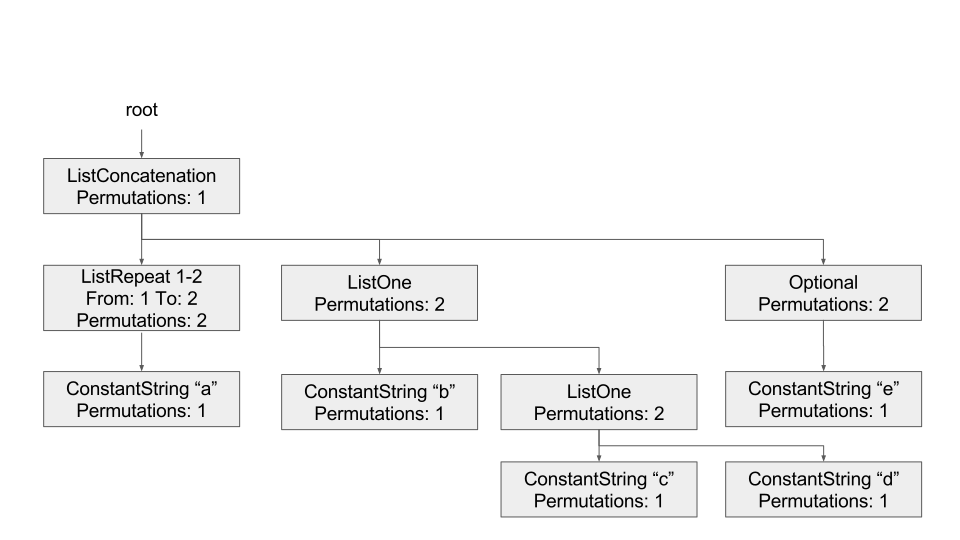
\includegraphics[width=1.0\textwidth]{images/tavor-all-permutation-token-graph.pdf}
\caption{AllPermutations example token graph}
\label{fig:all-perm-token-graph}
\end{figure}

\begin{table}[bt]
\caption{Computing PermutationsAll for different token types}
\label{table:compute-All-perms}
\center
\begin{tabular}{| l | l |}
\hline
  \textbf{Token Type}
& \textbf{Formula}
\tabularnewline
\hline
  Concatenation
& $\prod_{i=1}^{token.NumChildren} Token.Child(i).PermutationsAll()$
\tabularnewline
\hline
  Repeat
& $\sum_{i=From}^{To} Token.Child().PermutationsAll()^i$
\tabularnewline
\hline
  One
& $\sum_{i=0}^{token.NumChildren} Token.Child(i).PermutationsAll()$
\tabularnewline
\hline
  Optional
& $1 + token.Child().PermutationsAll()$
\tabularnewline
\hline
  String
& $1$
\tabularnewline
\hline
\end{tabular}
\end{table}

\begin{listing}
\caption{Permutation of AllPermutations example token graph}
\label{lst:permutations-allperm-token-graph}
\begin{gocode}
ab
aab
ac
aac
ad
aad
abe
aabe
ace
aace
ade
aade
\end{gocode}
\end{listing}

To iterate over all permutations of a token graph we view each token as a single digit in its own numeral system. In common numeral systems every digit has a fixed range. For instance, the decimal numeral system allows digits from 0 to 9. When incrementing a number over its range in one of those systems, a digit propagates an overflow to its neighboring higher digit and resets itself to the first digit of its range. Figure~\ref{fig:inc-decade-system} illustrates this propagation in the decimal numeral system on the calculations $0+1=1$, where no propagation takes place, $9+1=10$, where one digit propagates and $99+1=100$, where two digits propagate their overflow. A very similar concept is applied on token graphs when iterating over their permutations. In contrast to common number systems, each token may have a different range of values, i.e., an Optional Token can have the values $0$ and $1$ while a Repeat Token from 0 to 10 may have values from $0$ to $10$. In common numeral systems each digit has at most two neighboring digits, in comparison each token in a token graph may have a parent, siblings as well as child tokens which all need to be considered when calculating the next permutation.

\begin{figure}
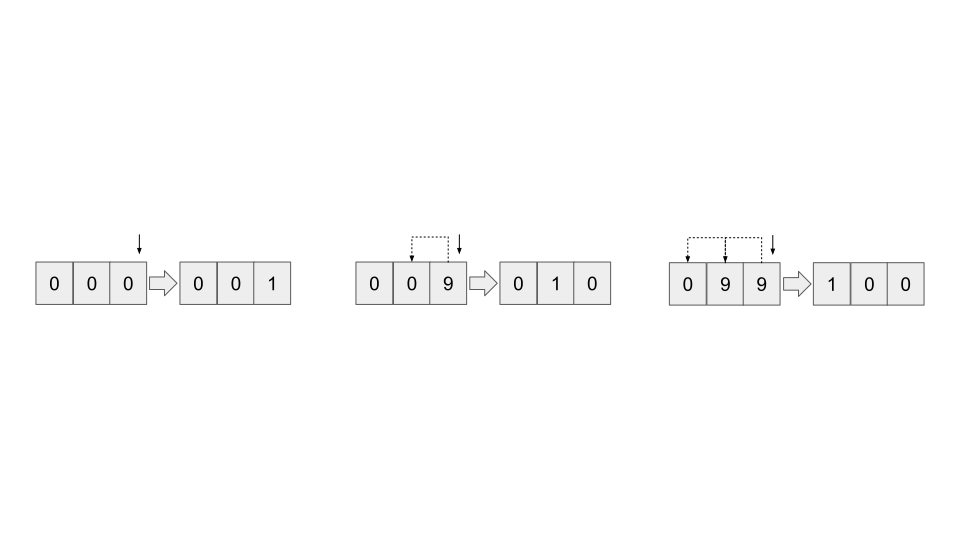
\includegraphics[width=1.0\textwidth]{images/tavor-increment-decade-system.pdf}
\caption{Incrementing in the decimal numeral system}
\label{fig:inc-decade-system}
\end{figure}

For calculating the next fuzzing iteration, i.e., the next permutation of the token graph, the AllPermutations strategy applies the following procedure on each token:
\begin{itemize}
\item If a token has children, first try to increment the permutation of its children. In case no overflow takes place, the next permutation has been successfully calculated.
\item If there are no children, or incrementing their current permutation results in an overflow, try to increment the current token's permutation. In case no overflow takes place, the next permutation has been successfully calculated.
\item If incrementing the permutation of the current token results in an overflow, propagate this overflow either to the neighboring higher sibling, or in case there are no siblings, the parent token. If the current token is the root token, this means the last permutation has been reached.
\end{itemize}

Figure~\ref{fig:all-perm-example} depicts the individual steps of the AllPermutations fuzzing strategy for the token graph shown in Figure~\ref{fig:all-perm-token-graph}. The solid arrows symbolize an increment instruction for a token, and the dashed arrows are used to depict the propagation of an overflow. The token graph is initialized with value 0 for all of its tokens, which represents the permutation \enquote{ab}. In order to step to the next permutation first an increment command is sent to the root token in iteration 0, which propagates this increment to its first child token the Repeat Token, which in turn also propagates to its child the String Token \enquote{a}. A String Token has only one permutation, hence, the increment command overflows setting the Repeat Token to value $1$, resulting in the permutation \enquote{aab}. In iteration 1 the same computation takes place, except that this time also the Repeat Token overflows setting the first One token to value $1$, resulting in permutation \enquote{ac}. This process continues until iteration 11, where the root token itself reports an overflow, hence no more permutations are available.

\begin{figure}[ht]
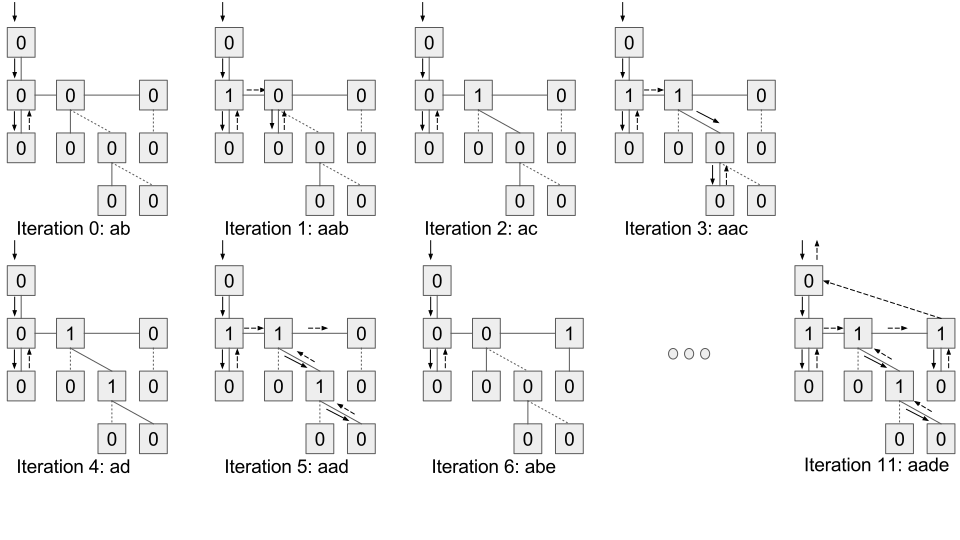
\includegraphics[width=1.0\textwidth]{images/tavor-all-permutations-example.pdf}
\caption{AllPermutations Iterations}
\label{fig:all-perm-example}
\end{figure}

Please refer to Appendix~\ref{chapter:AppendixTavorFramework} Listing~\ref{lst:pseudo-code-all-perm-strat} and Listing~\ref{lst:pseudo-code-all-perm-strat-helper} for the pseudo code of the AllPermutations fuzzing strategy.

\section{Fuzzing Filters}
\label{sec:fuzzingFilters}

In order to mutate a token graph, i.e., apply mutation-based fuzzing, the \textsc{Tavor framework} offers \emph{fuzzing filters}. Fuzzing filters do not change a specific permutation, but alter all permutations that may be generated with a specific token graph. All fuzzing filters need to implement the following interface:

\begin{center} \texttt{type Filter func(token Token) (Token, error)} \end{center}

This interface specifies a generic function, which applies the given filter onto a single token that is passed to the function. Therefore, the function's concern is only one token at a time. If an error is encountered during the filter execution, the error return argument is uninitialized. On success a replacement for the token is returned. If this replacement is not \texttt{nil}, it will replace the original token. Consider, for instance, a very basic filter that replaces each occurrence of the string \enquote{old} with the new constant string \enquote{new}. A possible implementation of this filter is shown in Listing~\ref{lst:tavor-example-filter}.

\begin{listing}[ht]
\caption{Sample Filter}
\label{lst:tavor-example-filter}
\begin{gocode}
func NewSampleFilter(token Token) (Token, error) {
	c, ok := token.(*String)
	if !ok || c.String() != "old" {
		return nil, nil
	}

	return NewString("new"), nil
}
\end{gocode}
\end{listing}

The \textsc{Tavor framework} offers a register function for fuzzing filters, which works along the same lines as the register function for fuzzing strategies. It allows to register filters based on an identifier, which can later on be used within the framework. The sample filter of Listing~\ref{lst:tavor-example-filter} can be registered with the \textsc{Tavor framework} using the code shown in Listing~\ref{lst:register-sample-filter}.

\begin{listing}[ht]
\caption{Registering the sample filter}
\label{lst:register-sample-filter}
\begin{gocode}
func init() {
	filter.Register("SampleFilter", NewSampleFilter)
}
\end{gocode}
\end{listing}

Applying a filter can be done manually or using the \emph{ApplyFilters} function. An excerpt of this function is shown in Listing~\ref{lst:func-apply-filters}. ApplyFilters traverses the graph using a queue of pairs holding the token to process and its parent. The root token of the input token graph is special, in the sense, that it does not have a parent. The inner loop in Lines~5-23 successively applies the passed in filters and alters the input token graph in case a replacement for one of its tokens has been found. Line~22 pushes the child tokens of the currently processed token onto the queue, ensuring that the whole graph is traversed.

\begin{listing}
\caption{Auxiliary function ApplyFilters}
\label{lst:func-apply-filters}
\begin{gocode}
func ApplyFilters(filters []Filter, root Token) Token {
	queue := NewQueue()
	queue.Push(&Pair{token: root, parent: nil})

	for !queue.Empty() {
		pair := queue.Pop()

		for i := range filters {
			replacement, _ := filters[i](pair.token)

			if replacement != nil {
				if pair.parent == nil {
					root = replacement
				} else {
					pair.parent.Replace(pair.token, replacement)
				}

				break
			}
		}

		addChildrenToQueue(queue, pair.token)
	}

	return root
}
\end{gocode}
\end{listing}

An example use case for fuzzing filters is the boundary-value analysis software testing technique, which commonly uses the first and last values of a range of values instead of the whole range. This reduces the amount of values that need to be tested. Consider a function which has one input parameter of the type integer. The parameter's valid values range from 1 to 100, i.e., there are 100 possible test candidates and thus 100 permutations. Boundary-value analysis may reduce these permutations to 1, 50 and 100, i.e., just three instead of 100 cases are tested. Additional to the first and last values, the middlemost value. The \textsc{Tavor framework} provides an implementation of this technique with the \texttt{PositiveBoundaryValueAnalysis} fuzzing filter. This fuzzing filter traverses the whole internal structure and replaces every range token with at most five boundary values, e.g., a range from -10 to 10 would result into -10, -1, 0, 1 and 10 therefore including the transition from negative to positive values. Another fuzzing filter, the \texttt{NegativeBoundaryValueAnalysis}, changes every range token to two integers, i.e., one representing its lower bound subtracted by one, and the other one, representing its upper bound incremented by one. Thus, resulting in values which are not valid in the original model but are useful to generate invalid data for testing. For the integer range from the previous example this would mean that the two integers 0 and 101 are generated.

\section{Reducing Strategies}
\label{sec:reducingStrategies}

A reducing strategy in the \textsc{Tavor framework} is a specific delta-debugging algorithm, which can be applied on the current permutation of a token graph. Individual reducing strategies may vary on the heuristic for walking through the token graph or on how the individual tokens are reduced. The reduction method is depending on the token type. For example a constant integer cannot be reduced any further but a repetition of optional strings can be minimized or even left out. All reducing strategies need to implement the following interface:

\begin{center} \texttt{type Strategy func(root Token) (chan bool, chan<- Feedback, error)} \end{center}

Every reducing strategy instance has to be associated on construction with exactly one token. This allows an instance to hold a dedicated state of the given token graph, which makes optimizations for multiple reducing operations and iterations possible. During construction a reducing strategy starts its first reduction step in a new coroutine and provides the following return arguments to control the reduction process:

\begin{enumerate}
\item A channel to synchronize the reduction progress. The reducing strategy writes to this channel to signal that a new reduced permutation is available, i.e., the current reduction iteration is completed. The caller of the strategy function is responsible to write to this channel as soon as it is able to process the next iteration. This passing of values is needed to avoid data races within the token graph. The channel must be closed when there are no more steps or the caller of the strategy wants to end the reduction process. Note that this can also occur right after receiving the channel, i.e., when there are no reductions at all.
\item A channel to receive feedback on the current iteration. The feedback answer \texttt{Good} communicates to the reducing strategy that the current iteration produced a successful result, e.g., that the result has the same outcome when it is used or is better than the last good result. The meaning of the feedback and the response of the strategy to the feedback are purely dependent on the application. Responses could be for example to proceed with a given optimization path or to simply end the whole reduction process, since it can be enough to find just one solution. The feedback answer \texttt{Bad} communicates exactly the opposite of \texttt{Good} to the strategy. This answer is often more complicated to handle, since it means that in some scenarios a revert of the current iteration to the last good iteration has to occur before the reduction process can continue.
\item An error indicating that the initialization of the strategy has not been successful. A reducing strategy may for instance return an error, in case the input token contains loops, as they are not supported by the \textsc{Tavor framework}.
\end{enumerate}

The \textsc{Tavor framework} offers as for the fuzzing strategies and filters a register function, which allows to register reducing strategies based on an identifier. This is especially needed for the Tavor CLI, which can execute a specific reducing strategy defined by a command line argument.

In order to provide a better understanding of the interactions between a reducing strategy and its caller, we walk through an example implementation of a fairly basic reducing strategy in Subsection~\ref{sec:basic-reduce-strategy}. Additionally, we offer in Section~\ref{sec:linear-reduce-strategy} the pseudo code of the linear reducing strategy, which is provided by the \textsc{Tavor framework}.

\subsection{Basic Example reducing strategy}
\label{sec:basic-reduce-strategy}

Consider a reducing strategy that searches the token graph for Repeat Tokens holding internally a String Token, reducing the repetition by one token for every reduction iteration. This reducing strategy is very simple and should demonstrate that reducing strategies can be added to the \textsc{Tavor framework} in a straight forward manner. It is a stateless strategy since every iteration can be executed independently of the previous one. Additionally, it is guaranteed to end, since only a finite amount of tokens is targeted without generating new ones.

Listing~\ref{lst:reduce-const-string-repetitions} shows the pseudo code for reducing repetitions of String Tokens. First the two channels for synchronization purposes are initialized. Next, a coroutine is defined in Lines~5-27, which makes use of the auxiliary function \texttt{Walk} of the \textsc{Tavor framework}, which receives two input parameters: the root token of the token graph that should be traversed and a function, which is called for each traversed token. This function is defined from Lines~6-24 and is responsible for the actual reduction process and synchronization with the caller. First, it checks in Line~7 whether the currently traversed token \texttt{token} is a Repeat Token referencing a String Token. If this is the case, the Repeat Token is stored in \texttt{repeat} and \texttt{ok} equals true. The loop from Lines~10-21 iterates over the number of available reductions, i.e., \texttt{repeat.Reduces()}, and tries in Line~13 to reduce the current token \texttt{repeat} by one of its referenced child tokens. This reduction is then reported in Line~16 to the caller by writing to the \texttt{continueReducing} channel. The feedback from the caller is processed in Line~17. Please note that this call blocks until the caller has written to the \texttt{feedbackReducing} channel. Finally, after the walk of the token graph has been completed the two synchronization channels are closed in Line~26.

\begin{listing}[ht]
\caption{Reduce String Token repetitions}
\label{lst:reduce-const-string-repetitions}
\begin{gocode}
func NewSampleStrategy(root Token) (chan bool, chan<- ReduceFeedbackType, error) {
	continueReducing := make(chan bool)
	feedbackReducing := make(chan ReduceFeedbackType)

	go func() {
		err := Walk(root, func(tok Token) error {
			repeat, ok := isRepeatingString(tok)
			if !ok { return nil }

			for i := repeat.Reduces() - 1; i >= 0; {
				found := false
				l := len(repeat.String())
				found, i := reduceByOne(repeat, l, i)
				if !found { break }

				continueReducing <- true
				feedback, ok := <-feedbackReducing
				if feedback == strategy.Good { return Done }
				if !ok { return nil }
				if _, ok := <-continueReducing; !ok { return nil }
			}

			return nil
		})
		if err != nil && err != Done { panic(err) }
		close(continueReducing); close(feedbackReducing)
	}()

	return continueReducing, feedbackReducing, nil
}
\end{gocode}
\end{listing}

Listing~\ref{lst:callee-reduce-const-string-repetitions} shows a matching counterpart to the sample reducing strategy of Listing~\ref{lst:reduce-const-string-repetitions}. First it initializes a concatenation list, which contains four Repeat Tokens each referencing a String Token in Lines~2-11. Next, it constructs the sample reducing strategy in Line~14. It concludes with processing the reduce steps in Lines~17-27, signaling the reducing strategy it should keep reducing until a length smaller or equal to ten is reached. When this function is executed it produces the output shown in Listing~\ref{lst:output-reduce-const-string-repetitions}, which shows that the Walk function first visits the Repeat Token referencing the string \enquote{a}, which is reduced until no \enquote{a} is left. Next the Repeat Token referencing the String Token \enquote{b} is processed, which is reduced until its minimum length of one is reached. This process continues until the token \texttt{doc} holds the value \enquote{bcccccccdd}, which has the target length of 10.

\begin{listing}[ht]
\caption{Callee of example reducing strategy}
\label{lst:callee-reduce-const-string-repetitions}
\begin{gocode}
func main() {
	aRepeat := NewRepeat(NewString("a"), 0, 100)
	aRepeat.Permutation(6)
	bRepeat := NewRepeat(NewString("b"), 1, 100)
	bRepeat.Permutation(4)
	cRepeat := NewRepeat(NewString("c"), 7, 100)
	cRepeat.Permutation(8)
	dRepeat := NewRepeat(NewString("d"), 1, 100)
	dRepeat.Permutation(1)

	var root Token = lists.NewConcatenation(aRepeat, bRepeat, cRepeat, dRepeat)
	fmt.Println(root.String())

	continueFuzzing, feedbackReducing, err := NewSampleStrategy(root)
	if err != nil { panic(err) }

	for i := range continueFuzzing {
		out := root.String()
		fmt.Println(out)

		if len(out) <= 10 {
			feedbackReducing <- strategy.Good
		} else {
			feedbackReducing <- strategy.Bad
		}
		continueFuzzing <- i
	}
}
\end{gocode}
\end{listing}

\begin{listing}[ht]
\caption{Command line output of example reducing strategy}
\label{lst:output-reduce-const-string-repetitions}
\begin{gocode}
aaaaaabbbbbcccccccccccccccdd
aaaaabbbbbcccccccccccccccdd
aaaabbbbbcccccccccccccccdd
aaabbbbbcccccccccccccccdd
aabbbbbcccccccccccccccdd
abbbbbcccccccccccccccdd
bbbbbcccccccccccccccdd
bbbbcccccccccccccccdd
bbbcccccccccccccccdd
bbcccccccccccccccdd
bcccccccccccccccdd
bccccccccccccccdd
bcccccccccccccdd
bccccccccccccdd
bcccccccccccdd
bccccccccccdd
bcccccccccdd
bccccccccdd
bcccccccdd
\end{gocode}
\end{listing}

Finally, the strategy can be registered as a framework-wide usable strategy using the code shown in Listing~\ref{lst:register-sample-strategy}. This registration is, for instance, necessary in order to use the sample strategy when working with the \textsc{Tavor CLI}.

\begin{listing}[ht]
\caption{Registering the sample strategy}
\label{lst:register-sample-strategy}
\begin{gocode}
func init() {
	strategy.Register("SampleStrategy", NewSampleStrategy)
}
\end{gocode}
\end{listing}

\subsection{The Linear reducing strategy}
\label{sec:linear-reduce-strategy}

The Linear reducing strategy reduces data based on a linear search. In contrast to the sample strategy from the previous section, this strategy does not rely on specific token types for reduction, but solely operates on the following interfaces:

\begin{itemize}
\item The \texttt{Reduce Interface} is implemented by tokens which may be reduced. The method \texttt{Reduces() int} is used to determine the number of available reductions and the method \texttt{Reduce(i int)} is available to set a specific reduction.
\item The \texttt{Forward Interface} is implemented by tokens which wrap other tokens. The method \texttt{Get()} is provided by this interface in order to access the wrapped token.
\item The \texttt{List Interface} is implemented by tokens that wrap several tokens. The method \texttt{Len()} informs about the number of wrapped child tokens and the method \texttt{Get(i int)} returns a child specified by its index \texttt{i}.
\end{itemize}

Consider Listing~\ref{lst:lin-reduce-strat}, it shows the top level implementation of the Linear reducing strategy. It starts off by creating the two synchronization channels \texttt{contin} and \texttt{feedback}. As with the sample reducing strategy the actual reduction is performed in a coroutine. Line~5 uses the auxiliary function \texttt{getReductionListFromTree(root)}, which traverses the token graph referenced by \texttt{root} and returns a list of tokens which can be reduced. This list of tokens is passed on to the auxiliary function \texttt{reduce(contin, feedback, list)}, which reduces these tokens and communicates over the channels \texttt{contin} and \texttt{feedback} with the caller of the Linear reducing strategy.

\begin{listing}[ht]
\caption{Linear reducing strategy}
\label{lst:lin-reduce-strat}
\begin{gocode}
func NewLinear(root token.Token) (chan bool, chan<- ReduceFeedbackType, error) {
	contin := make(chan bool)
	feedback := make(chan ReduceFeedbackType)
	go func() {
		list := getReductionListFromTree(root)
		if !reduce(contin, feedback, list) {
			return
		}
		close(contin)
		close(feedback)
	}()
	return contin, feedback, nil
}
\end{gocode}
\end{listing}

The pseudo code of the auxiliary function \texttt{getReductionListFromTree} is shown in Listing~\ref{lst:lin-reduce-strat-traverse-graph}. It uses a queue to traverse the token graph rooted in the token \texttt{root}. The loop starting in Line~7 searches for tokens implementing the \texttt{Reduce Interface} and adds them to the list of reducible tokens. Tokens wrapping child tokens are dealt with in Lines~9-14 by unwrapping them and adding them to the queue for later procession.

\begin{listing}[ht]
\caption{Traversing of the token graph}
\label{lst:lin-reduce-strat-traverse-graph}
\begin{gocode}
func getReductionListFromTree(root Token) (list []ReduceToken) {
	queue := NewQueue()
	queue.Push(root)
	for !queue.Empty() {
		token := queue.Pop()
		switch t := token.(type) {
		case ReduceToken:
			list = append(list, token)
		case ForwardToken:
			queue.Push(t.Get())
		case ListToken:
			for i := t.Len() - 1; i >= 0; i-- {
				queue.Push(t.Get(i))
			}
		}
	}
	return list
}
\end{gocode}
\end{listing}

Listing~\ref{lst:lin-reduce-strat-reduce} shows the pseudo code of an excerpt of the \texttt{reduce} method. It walks through the tokens stored in \texttt{list} and tries to find a suitable reduction of the current token in the loop from Lines~3-12. The auxiliary function \texttt{nextStep} handles the synchronization with the reducing strategy caller via the channels \texttt{contin} and \texttt{feedback}, which is done along the same lines as for the sample reducing strategy in the previous subsection. Please note that \texttt{c.Reduce(c.Reduces()-1)} is always equal to the initial value of \texttt{c}, i.e., if no suitable reduction is found the last iteration of the inner loop performs the restoration of the initial value of \texttt{c}. Finally the switch-statement in Line~13 is responsible for recursively calling the \texttt{reduce} method to Forward and List tokens. Consider, for instance, a token graph which has as its root a Repeat Token referencing another reducible token. The root Repeat Token is reducible, hence it will be in the list of reducible tokens during the first call of method \texttt{reduce}. Its referenced child is not part of that list, hence a recursive call of method \texttt{reduce} is necessary to also process this token.

\begin{listing}[ht]
\caption{Performing the reduction}
\label{lst:lin-reduce-strat-reduce}
\begin{gocode}
func reduce(contin chan bool, feedback <-chan ReduceFeedbackType, tree []ReduceToken) bool {
	for _, c := range tree {
		for i := 0; i < c.Reduces(); i++ {
			c.Reduce(i)
			contin, feedback := nextStep(contin, feedback)
			if !contin {
				return false
			} else if feedback == Good {
				break
			}
			c.reduction++
		}
		switch t := c.(type) {
		case ForwardToken:
			children := getReductionListFromTree(c.Get())
			reduce(contin, feedback, children)
		case ListToken:
			for i := t.Len() - 1; i >= 0; i-- {
				children := getReductionListFromTree(c.Get(i))
				reduce(contin, feedback, children)
			}
		}
	}
	return true
}
\end{gocode}
\end{listing}

\chapter{\textsc{Tavor Format}}
\label{chapter:tavorFormat}

The \textsc{Tavor format} is an EBNF-like notation which allows the definition of data, such as file formats and protocols, without the need of programming. It is the default format of the Tavor CLI of Chapter~\ref{chapter:tavorCLI} and supports every feature of the framework, which has been introduced in Chapter~\ref{chapter:tavorFramework}. Each of the demonstrated features of the \textsc{Tavor format} is required to fully define the AIGER format.

The format is Unicode text encoded in UTF-8 and consists of terminal and non-terminal symbols which are called \texttt{tokens} throughout the \textsc{Tavor framework}. A more general definition of \texttt{tokens} can be found in Section~\ref{sec:tokens}.

\section{Token Definition}
\label{sec:tokenDefinition}

Every \texttt{token} in the format belongs to a definition of \texttt{non-terminal token} which consists of a unique case-sensitive name and its definition part. Both are separated by exactly one equal sign. Syntactical white spaces are ignored. Every \texttt{token definition} is by default declared in one line. A line ends with a new-line character.

To give an example, the format in Listing~\ref{lst:tavorHelloWorld} declares the \texttt{START token} with the \texttt{String Token} \enquote{Hello World} as its definition.

\begin{listing}
\caption{\textsc{Tavor}'s Hello World}
\label{lst:tavorHelloWorld}
\begin{gocode}
START = "Hello World"
\end{gocode}
\end{listing}

\texttt{Token names} have the following constraints: Each \texttt{token name} has to start with a letter, and can only consist of letters, digits and the underscore sign \enquote{\char`_}. Additionally, a \texttt{token name} has to be unique. It is also not allowed to declare a \texttt{token} and never use it. The \texttt{START token} is the only exception, which is used as the entry point of the format. Hence it defines the beginning of the format and is therefore required for every format definition.

Sequential listed \texttt{tokens} in the definition part of a \texttt{token definition} are automatically concatenated. The example in Listing~\ref{lst:concatenationExample} concatenates to the string \enquote{This is a String Token and this 123 was a number token.}.

\begin{listing}
\caption{Example for a token concatenation}
\label{lst:concatenationExample}
\begin{gocode}
START = "This is a String Token and this " 123 " was a number token."
\end{gocode}
\end{listing}

A \texttt{token definition} can be sometimes too long or poorly readable, it can be therefore split into multiple lines by using a comma before the newline character as shown in Listing~\ref{lst:multiLineTokenDefinitionExample}. The \texttt{token definition} ends at the string \enquote{definition.} since there is no comma before the newline character. Listing~\ref{lst:multiLineTokenDefinitionExample} also highlights that syntactical white spaces are ignored and can be used to make a format definition more human-readable.

\begin{listing}
\caption{Example for a multi-line token definition}
\label{lst:multiLineTokenDefinitionExample}
\begin{gocode}
START = "This",
        "is",
        "a",
        "multi line",
        "definition."
\end{gocode}
\end{listing}

The \textsc{Tavor format} supports two kinds of comments. \texttt{Line comments} start with the character sequence \enquote{//} and end at the next new-line character. \texttt{General comments} start with the character sequence \enquote{/*} and end at the character sequence \enquote{*/}. A general comment can therefore contain new-line characters and can be used between \texttt{token definition} and \texttt{tokens}. Both kinds of comments are illustrated in Listing~\ref{lst:commentsExample}.

\begin{listing}
\caption{Example for different kinds of comments}
\label{lst:commentsExample}
\begin{gocode}
/*

This is a general comment
which can have
multiple lines.

*/

START = "This is a string." // This is a line comment.

// This is also a line comment.
\end{gocode}
\end{listing}

\section{Terminal Tokens}
\label{sec:terminalTokens}

\texttt{Terminal tokens} are the constants of the \textsc{Tavor format}. The format supports two kinds of \texttt{terminal tokens}: numbers and strings. Every other token that is not a \texttt{terminal token}, such as \texttt{tokens} of definitions, is called a \texttt{non-terminal token}.

\texttt{Number tokens} allow only positive decimal integers, which are written as a sequence of digits as shown in Listing~\ref{lst:numberTokenExample}.

\begin{listing}
\caption{Example for a number token}
\label{lst:numberTokenExample}
\begin{gocode}
START = 123
\end{gocode}
\end{listing}

\texttt{String Tokens} are character sequences between double quote characters and can consist of any UTF-8 encoded character except the new-line, the double quote and the backslash characters which have to be escaped with a backslash character. An example can be seen in Listing~\ref{lst:stringTokenExample}.

\begin{listing}
\caption{Example for a String Token}
\label{lst:stringTokenExample}
\begin{gocode}
START = "The next word is \"quoted\" and next is a new line\n"
\end{gocode}
\end{listing}

Since \textsc{Tavor} is using \textsc{Go}'s text parser as foundation of its format parsing, the same rules for \enquote{interpreted string literals} as defined in \textsc{Go}'s language specification~\cite{2017_go_spec} apply to \texttt{String Tokens}.

Empty \texttt{String Token} are forbidden and lead to a format parsing error. The reason for this exceptions is the way \texttt{tokens} are utilized during parsing and delta-debugging, and is described in the repeat groups of Paragraph~\ref{par:groupRepeat} in more detail.

\section{Embedding of Tokens}
\label{sec:tokenEmbedding}

\texttt{Non-terminal tokens} can be embedded in the definition part by using the name of the referenced \texttt{token}. The example in Listing~\ref{lst:embeddingTokens} embeds the \texttt{token} \enquote{Text} into the \texttt{START token}. \texttt{Token names} declared in the global scope of a format definition can be used throughout the format regardless of their declaration position. Terminal and non-terminal tokens can be mixed as illustrated in Listing~\ref{lst:mixedTokensExample}.

\begin{listing}
\caption{Example for embedding tokens}
\label{lst:embeddingTokens}
\begin{gocode}
START = Text

Text = "Some text"
\end{gocode}
\end{listing}

\begin{listing}
\caption{Example for terminal and non-terminal tokens mixed in one format}
\label{lst:mixedTokensExample}
\begin{gocode}
Dot = "."

First  = 1 Dot
Second = 2 Dot
Third  = 3 Dot

START = First ", " Second " and " Third
\end{gocode}
\end{listing}

The \textsc{Tavor framework} and therefore the \textsc{Tavor format} differentiate between a \texttt{token reference}, which is the embedding of a \texttt{token} in a definition, and a \texttt{token usage}, which is the execution of a \texttt{token} during an operation such as fuzzing or delta-debugging. Listing~\ref{lst:tokenUsageTokenReferenceExample} illustrates the difference between a \texttt{token reference} and a \texttt{token usage}. The format defines two \texttt{tokens} called \enquote{Choice} and \enquote{List}. There exists one \texttt{token reference} of \enquote{Choice}, which can be found in the \enquote{List} definition, and two for \enquote{List}, which are both in the \texttt{START token} definition. Although \enquote{Choice} is in a \texttt{repeat group}, which in this example repeats the token \enquote{Choice} exactly twice, it is only referenced once. \enquote{List} has two \texttt{token usages} in this format while \enquote{Choice} has 4. Every \enquote{List} \texttt{token} does have two \enquote{Choice} usages because of the \texttt{repeat group} in the definition of \enquote{List}.

\begin{listing}
\caption{Example for a token reference and a token usage}
\label{lst:tokenUsageTokenReferenceExample}
\begin{gocode}
Choice = "a" | "b" | "c"

List = +2(Choice)

START = "1. list: " List "\n",
        "2. list: " List "\n"
\end{gocode}
\end{listing}

\section{Alternations}
\label{sec:alternation}

\texttt{Alternations} are defined by the pipe character \enquote{|} which separates two \texttt{alternation terms}. The example in Listing~\ref{lst:alternationExample} defines that the token \texttt{START} can either hold the strings \enquote{a}, \enquote{b} or \enquote{c}. An \texttt{alternation term} has its own scope which means that a sequence of \texttt{tokens} can be used.

\begin{listing}
\caption{Example for the alternation token}
\label{lst:alternationExample}
\begin{gocode}
START = "a" | "b" | "c"
\end{gocode}
\end{listing}

\texttt{Alternation terms} can be empty which allows more advanced definitions of formats. Listing~\ref{lst:alternationLoop} illustrates how to use an alternation to define a loop which can either hold the empty string or the strings \enquote{a}, \enquote{b}, \enquote{ab}, \enquote{aab} or any amount of \enquote{a} characters ending with an optional \enquote{b} character.

\begin{listing}
\caption{Example for loop using an alternation}
\label{lst:alternationLoop}
\begin{gocode}
A = "a" A | B |
B = "b"

START = A
\end{gocode}
\end{listing}

\section{Groups}
\label{sec:groups}

\texttt{Tokens} can be arranged using \texttt{token groups} by using parenthesis beginning with the opening parenthesis character \enquote{(} and ending with the closing parenthesis character \enquote{)}. A \texttt{group} is a \texttt{token} on its own and can be therefore mixed with other \texttt{tokens}. Additionally, a \texttt{group} starts a new scope between its parenthesis and can therefore hold a sequence of \texttt{tokens}. The \texttt{tokens} between the parenthesis are called the \texttt{group body}. Listing~\ref{lst:groupToken} illustrates the usage of a \texttt{token group} by declaring that the \texttt{START token} can either hold the string \enquote{a c} or \enquote{d c}. \texttt{Groups} can be nested as illustrated in Listing~\ref{lst:nestedGroups}, which defines a number with one to three digits. \texttt{Groups} can have modifiers which give a \texttt{group} additional abilities. The following sections introduces these modifiers.

\begin{listing}
\caption{Example for a group token}
\label{lst:groupToken}
\begin{gocode}
START = ("a" | "d") " c"
\end{gocode}
\end{listing}

\begin{listing}
\caption{Example for nested groups}
\label{lst:nestedGroups}
\begin{gocode}
Digit = 0 | 1 | 2 | 3 | 4 | 5 | 6 | 7 | 8 | 9

START = Digit (Digit (Digit | ) | )
\end{gocode}
\end{listing}

\paragraph{Optional group}
\label{subsec:groupOptional}

The \texttt{optional group} has the question mark \enquote{?} as modifier and allows the whole \texttt{group token} to be optional. The \texttt{START token} in Listing~\ref{lst:optionalGroup} can either hold the strings "a" or "a b".

\begin{listing}
\caption{Example for an optional group}
\label{lst:optionalGroup}
\begin{gocode}
START = "a" ?(" b")
\end{gocode}
\end{listing}

\paragraph{Repeat group}
\label{par:groupRepeat}

The default modifier for the \texttt{repeat group} is the plus character \enquote{+}. The repetition is executed by default at least once. In Listing~\ref{lst:groupRepeat} the string \enquote{a} is repeated and the \texttt{START token} can therefore hold any amount of \enquote{a} characters but at least one.

\begin{listing}
\caption{Example for a repeat group}
\label{lst:groupRepeat}
\begin{gocode}
START = +("a")
\end{gocode}
\end{listing}

Since repeated empty \texttt{tokens} lead to infinite steps during parsing and delta-debugging, a parsing error is issued if such \texttt{tokens} are encountered. This includes \texttt{optional groups} or \texttt{alternations} with at least one empty term inside a \texttt{Repeat Token}. The \texttt{repeat group} repeats by default from one to infinite times. The repetition can be altered with arguments to the modifier. Listing~\ref{lst:groupFixedRepeat} repeats the string \enquote{a} exactly twice. The \texttt{START token} can therefore only hold the string \enquote{aa}. It is also possible to define a repetition range. Listing~\ref{lst:groupRangedRepeat} repeats the string \enquote{a} at least twice but at most four times. This means that the \texttt{START token} can either hold the strings \enquote{aa}, \enquote{aaa} or \enquote{aaaa}. The \enquote{from} and \enquote{to} arguments can be empty too. They are then set to their default values. Listing~\ref{lst:groupEmptyFromArgumentRepeatGroup} repeats the string \enquote{a} at least once and at most four times. Listing~\ref{lst:groupEmptyToArgumentRepeatGroup} repeats the string \enquote{a} at least twice. Listing~\ref{lst:groupOptionalRepeat} illustrates the \texttt{optional repeat group} modifier. The \texttt{START token} can either hold the strings \enquote{a}, \enquote{ab}, \enquote{abb} or any amount of \enquote{b} characters prefixed by an "a" character.

\begin{listing}
\caption{Example for a fixed repeat group}
\label{lst:groupFixedRepeat}
\begin{gocode}
START = +2("a")
\end{gocode}
\end{listing}

\begin{listing}
\caption{Example for a ranged repeat group}
\label{lst:groupRangedRepeat}
\begin{gocode}
START = +2,4("a")
\end{gocode}
\end{listing}

\begin{listing}
\caption{Example for an empty ``from'' argument for a ranged repeat group}
\label{lst:groupEmptyFromArgumentRepeatGroup}
\begin{gocode}
START = +,4("a")
\end{gocode}
\end{listing}

\begin{listing}
\caption{Example for an empty ``to'' argument for a ranged repeat group}
\label{lst:groupEmptyToArgumentRepeatGroup}
\begin{gocode}
START = +2,("a")
\end{gocode}
\end{listing}

\begin{listing}
\caption{Example for an optional repeat group}
\label{lst:groupOptionalRepeat}
\begin{gocode}
START = "a" *("b")
\end{gocode}
\end{listing}

\paragraph{Permutation group}
\label{subsec:groupPermutation}

The \enquote{@} is the permutation modifier which is combined with an alternation in the group body. Each alternation term will be executed exactly once but the order of execution is non-relevant. In Listing~\ref{lst:groupPermutation} the \texttt{START token} can either hold \enquote{123}, \enquote{132}, \enquote{213}, \enquote{231}, \enquote{312} or \enquote{321}.

\begin{listing}
\caption{Example for a permutation group}
\label{lst:groupPermutation}
\begin{gocode}
START = @(1 | 2 | 3)
\end{gocode}
\end{listing}

\section{Character Classes}
\label{sec:characterClasses}

\texttt{Character class tokens} can be directly compared to character classes of regular expressions used in most programming languages. A \texttt{character class token} begins with the left bracket \enquote{[} and ends with the right bracket \enquote{]}. The content between the brackets is called a pattern and can consists of almost any UTF-8 encoded character, escape character, special escape character and range. In general the \texttt{character class token} can be seen as a shortcut for an \texttt{alternation}. The definition in Listing~\ref{lst:characterClassExample} illustrates the usage of a \texttt{character class} by defining that the \texttt{START token} holds either the strings \enquote{a}, \enquote{b} or \enquote{c}.

\begin{listing}
\caption{Example for a character class token}
\label{lst:characterClassExample}
\begin{gocode}
START = [abc]
\end{gocode}
\end{listing}

\paragraph{Escape Characters}
\label{subsec:characterClassEscapeCharacters}

Table~\ref{table:escapeCharacters} holds all \texttt{escape characters} which are UTF-8 encoded characters that are not directly allowed within a \texttt{character class} pattern. Their equivalent escape sequence has to be used instead. Listing~\ref{lst:escapeCharacterExample} defines that the \texttt{START token} can hold only white space characters.

\begin{table}[H]
\caption{Escape characters for character classes}
\label{table:escapeCharacters}
\center
\begin{tabular}{| l | l |}
\hline
  \textbf{Character}
& \textbf{Escape sequence}
\tabularnewline
\hline
  \enquote{-}
& \enquote{\textbackslash-}
\tabularnewline
\hline
  \enquote{\textbackslash}
& \enquote{\textbackslash\textbackslash}
\tabularnewline
\hline
  form feed
& \enquote{\textbackslash{}f}
\tabularnewline
\hline
  newline
& \enquote{\textbackslash{}n}
\tabularnewline
\hline
  return
& \enquote{\textbackslash{}r}
\tabularnewline
\hline
  tab
& \enquote{\textbackslash{}t}
\tabularnewline
\hline
\end{tabular}
\end{table}

\begin{listing}
\caption{Example for escape characters in character classes}
\label{lst:escapeCharacterExample}
\begin{gocode}
START = +([ \t\n\r\f])
\end{gocode}
\end{listing}

Since some characters can be hard to type and read the \enquote{\textbackslash{}x} escape sequence can be used to define them with their hexadecimal code points. Either only two hexadecimal characters are used in the form of \enquote{\textbackslash{}x0A} or when more then two hexadecimal digits are needed the form \enquote{\textbackslash{}x\string{0AF\string}} has to be used. The second form allows up to eight digits and is therefore fully Unicode ready. Unicode usage is illustrated in Listing~\ref{lst:hexadecimalCharacterClassExample}, which either holds the Unicode character \enquote{/} or \enquote{\smiley}.

\begin{listing}
\caption{Example for hexadecimal code points in character classes}
\label{lst:hexadecimalCharacterClassExample}
\begin{gocode}
START = [\x2F\x{263A}]
\end{gocode}
\end{listing}

\paragraph{Character Class Ranges}
\label{subsec:characterClassRanges}

\texttt{Character class ranges} can be defined using the \enquote{-} character. A \texttt{range} holds all characters defined by UTF-8 starting from the character before the \enquote{-} to ending at the character after the \enquote{-}. Both characters have to be either an UTF-8 encoded or an escaped character. The starting character must have a lower value than the ending character. The usage of \texttt{Character classes} is illustrated in Listing~\ref{lst:characterClassRange} which defines a number with one digit.

\begin{listing}
\caption{Example for a character class range}
\label{lst:characterClassRange}
\begin{gocode}
START = [0-9]
\end{gocode}
\end{listing}

\paragraph{Special Escape Characters}
\label{subsec:specialEscapeCharacters}

\texttt{Special escape characters} combine many characters into one \texttt{escape character}. Table~\ref{table:specialEscapeCharacters} lists all implemented \texttt{special escape characters}.

\begin{table}[H]
\caption{Special escape characters for character classes}
\label{table:specialEscapeCharacters}
\center
\begin{tabular}{| l | l | l |}
\hline
  \textbf{Escape character}
& \textbf{Character class}
& \textbf{Description}
\tabularnewline
\hline
  \enquote{\textbackslash{}d}
& \enquote{[0-9]}
& Holds a decimal digit character
\tabularnewline
\hline
  \enquote{\textbackslash{}s}
& \enquote{[ \textbackslash{}f\textbackslash{}n\textbackslash{}r\textbackslash{}t]}
& Holds a white space character
\tabularnewline
\hline
  \enquote{\textbackslash{}w}
& \enquote{$[a-zA-Z0-9\textunderscore]$}
& Holds a word character
\tabularnewline
\hline
\end{tabular}
\end{table}

\section{Token Attributes}
\label{sec:tokenAttributes}

Some \texttt{tokens} define attributes which can be used in a definition by prefixing the dollar sign \enquote{\$} to their name and appending a dot followed by the attribute name. Listing~\ref{lst:tokenAttributeExample} illustrates \texttt{token attributes} using the \enquote{Count} attribute, which holds the count of the token's direct children. The format holds for example the string "The number 56 has 2 digits".

\begin{listing}
\caption{Example for a token attribute using the ``Count'' attribute}
\label{lst:tokenAttributeExample}
\begin{minted}[
  mathescape,
  linenos,
  numbersep=5pt,
  breaklines,
  bgcolor=white,
]{go}
Number = +([0-9])
START = "The number " Number " has " $Number.Count " digits"
\end{minted}
\end{listing}

Some \texttt{token attributes} can have arguments. A \texttt{token argument list} begins with the opening parenthesis \enquote{(} and ends with the closing parenthesis \enquote{)}, and holds \enquote{token argument parameters} which are separated by commas. All \texttt{list tokens} have for example the \enquote{Item} attribute, which holds one child of the token. The \enquote{Item} attribute has one argument which is the index of the child starting from the index zero, and is illustrated in Listing~\ref{lst:tokenAttributeParameterExample}. The format holds the string "The letter with the index 1 is b".

\begin{listing}
\caption{Example for attribute parameters using the ``Item'' attribute}
\label{lst:tokenAttributeParameterExample}
\begin{minted}[
  mathescape,
  linenos,
  numbersep=5pt,
  breaklines,
  bgcolor=white,
]{go}
Letters = "a" "b" "c"
START = "The letter with the index 1 is " $Letters.Item(1)
\end{minted}
\end{listing}

A \texttt{list token} is a \texttt{token} which has in its definition either only a sequence of \texttt{tokens} or exactly one \texttt{repeat group token}. Table~\ref{table:listTokenAttributes} shows the \texttt{token attributes} that can be utilized by \texttt{list tokens}.

\begin{table}[H]
\caption{Token attributes for list tokens}
\label{table:listTokenAttributes}
\center
\begin{tabulary}{\textwidth}{| l | l | J |}
\hline
  \textbf{Attribute}
& \textbf{Arguments}
& \textbf{Description}
\tabularnewline
\hline
  \enquote{Count}
& -
& Holds the count of the token's direct children.
\tabularnewline
\hline
  \enquote{Item}
& \enquote{i}
& Holds a direct child of the token with the index \enquote{i}.
\tabularnewline
\hline
  \enquote{Unique}
& -
& Chooses at random a direct child of the token and embeds it. The choice is unique for every reference of the token.
\tabularnewline
\hline
\end{tabulary}
\end{table}

\paragraph{Scope of Attributes}
\label{subsec:scopeOfAttributes}

The \textsc{Tavor format} allows the usage of \texttt{token attributes} as long as the referenced \texttt{token} exists in the current scope.

Two kinds of scopes exist: The \texttt{global scope} is the scope of the whole format definition. An entry of the \texttt{global scope} is set by the nearest child \texttt{token reference} to the \texttt{START token}. The \texttt{local scope} is the scope held by a definition, \texttt{group} or any other \texttt{token} which holds its own scope. \texttt{Local scopes} are initialized with entries from their parent scope at the time of the creation of the new \texttt{local scope}. Listing~\ref{lst:scopeExample} illustrates this behavior which can for example hold the string \enquote{1 a 1(1 aa 2)1 aaa 3}. The \texttt{List} token is used trice in this example. The first usage leads to the value \enquote{a}, the second to \enquote{aa} and the third to \enquote{aaa}. Depending on which list is visible in the current scope \enquote{\$List.Count} results in another value. This example showcases that the scope of token \texttt{Inner} is not visible in the scope of the \texttt{START token}.

\begin{listing}
\caption{Example for scopes}
\label{lst:scopeExample}
\begin{minted}[
  mathescape,
  linenos,
  numbersep=5pt,
  breaklines,
  bgcolor=white,
]{go}
List = +,10("a")

Inner = "(" $List.Count " " List " " $List.Count ")"

START = $List.Count " " List " " $List.Count,
        Inner,
        $List.Count " " List " " $List.Count
\end{minted}
\end{listing}

\section{Typed Tokens}
\label{sec:typedTokens}

\texttt{Typed tokens} are a functional addition to regular \texttt{token definitions} of the \textsc{Tavor format}. They provide specific functionality which can be utilized by embedding them like regular \texttt{tokens} or through their additional \texttt{token attributes}. \texttt{Typed tokens} can be defined by prefixing the dollar sign \enquote{\$} to their name. They do not have a format definition on their right-hand side. Instead, a type and optional arguments written as key-value pairs, which are separated by a colon, define the \texttt{token}. Listing~\ref{lst:typedTokenExample} illustrates \texttt{typed tokens} with the definition of an \texttt{integer token}. The format definitions holds additions with random integers as numbers such as \enquote{47245 + 6160 + 6137}.

\begin{listing}
\caption{Example typed token using an integer token}
\label{lst:typedTokenExample}
\begin{minted}[
  mathescape,
  linenos,
  numbersep=5pt,
  breaklines,
  bgcolor=white,
]{go}
$Number Int

Addition = Number " + " (Number | Addition)

START = Addition
\end{minted}
\end{listing}

The range of the \enquote{Int} type can be bounded using arguments for the definition as shown in Listing~\ref{lst:typedTokenAttributesExample}, where the \texttt{token} \enquote{Number} is an integer within the range one to ten.

\begin{listing}
\caption{Example for typed token attributes}
\label{lst:typedTokenAttributesExample}
\begin{minted}[
  mathescape,
  linenos,
  numbersep=5pt,
  breaklines,
  bgcolor=white,
]{go}
$Number Int = from: 1,
              to:   10

Addition = Number " + " (Number | Addition)

START = Addition
\end{minted}
\end{listing}

\paragraph{Typed Token \texttt{Int}}
\label{subsec:typedTokensInt}

The \texttt{Int} type implements a random integer. Its optional \texttt{token arguments} are listed in Table~\ref{table:typedTokensIntOptionalArguments} and its \texttt{token attributes} are listed in Table~\ref{table:typedTokensIntArguments}.

\begin{table}[H]
\caption{Optional Token arguments for the ``Int'' typed token}
\label{table:typedTokensIntOptionalArguments}
\center
\begin{tabular}{| l | l |}
\hline
  \textbf{Arguments}
& \textbf{Description}
\tabularnewline
\hline
  \enquote{from}
& First integer value (defaults to 0)
\tabularnewline
\hline
  \enquote{to}
& Last integer value (defaults to $2^{31} - 1$)
\tabularnewline
\hline
\end{tabular}
\end{table}

\begin{table}[H]
\caption{Token attributes for the ``Int'' typed token}
\label{table:typedTokensIntArguments}
\center
\begin{tabular}{| l | l | l |}
\hline
  \textbf{Attribute}
& \textbf{Arguments}
& \textbf{Description}
\tabularnewline
\hline
  \enquote{Value}
& -
& Embeds a new token based on its parent
\tabularnewline
\hline
\end{tabular}
\end{table}

\paragraph{Typed Token \texttt{Sequence}}
\label{subsec:typedTokensSequence}

The \texttt{Sequence} type implements a generator for integers. Its optional \texttt{token arguments} are listed in Table~\ref{table:typedTokensSequenceOptionalArguments} and its \texttt{token attributes} are listed in Table~\ref{table:typedTokensSequenceArguments}.

\begin{table}[H]
\caption{Optional Token arguments for the ``Sequence'' typed token}
\label{table:typedTokensSequenceOptionalArguments}
\center
\begin{tabular}{| l | l |}
\hline
  \textbf{Arguments}
& \textbf{Description}
\tabularnewline
\hline
  \enquote{start}
& First sequence value (defaults to 1)
\tabularnewline
\hline
  \enquote{step}
& Increment of the sequence (defaults to 1)
\tabularnewline
\hline
\end{tabular}
\end{table}

\begin{table}[H]
\caption{Token attributes for the ``Sequence'' typed token}
\label{table:typedTokensSequenceArguments}
\center
\begin{tabulary}{\textwidth}{| l | l | J |}
\hline
  \textbf{Attribute}
& \textbf{Arguments}
& \textbf{Description}
\tabularnewline
\hline
  \enquote{Existing}
& -
& Embeds a new token holding one existing value of the sequence
\tabularnewline
\hline
  \enquote{Next}
& -
& Embeds a new token holding the next value of the sequence
\tabularnewline
\hline
  \enquote{Reset}
& -
& Embeds a new token which on execution resets the sequence
\tabularnewline
\hline
\end{tabulary}
\end{table}

\afterpage{\clearpage}

\section{Expressions}
\label{sec:expressions}

\texttt{Expressions} can be used in \texttt{token definitions} and allow dynamic and complex operations using \texttt{operators} who can have different numbers of \texttt{operands}. An \texttt{expressions} starts with the dollar sign \enquote{\$} and the opening curly brace \enquote{\{} and ends with the closing curly brace \enquote{\}}. Listing~\ref{lst:expressionExample} illustrates the simplest expression which is an addition.

\begin{listing}
\caption{Example expression}
\label{lst:expressionExample}
\begin{minted}[
  mathescape,
  linenos,
  numbersep=5pt,
  breaklines,
  bgcolor=white,
]{go}
START = ${1 + 2}
\end{minted}
\end{listing}

Every \texttt{operand} of an \texttt{operator} can be a token. The usual dollar sign for a \texttt{token attribute} can be omitted inside an \texttt{expression} as illustrated in Listing~\ref{lst:tokenAttributeInExpression}.

\begin{listing}
\caption{Example for a token attribute inside an expression}
\label{lst:tokenAttributeInExpression}
\begin{minted}[
  mathescape,
  linenos,
  numbersep=5pt,
  breaklines,
  bgcolor=white,
]{go}
$Number Int

START = ${Number.Value + 1}
\end{minted}
\end{listing}


\paragraph{Arithmetic Operators}
\label{subsec:arithmeticOperators}

\texttt{Arithmetic operators} which are shown in Table~\ref{table:arithmeticOperators} have two \texttt{operands} between the \texttt{operator} sign. \texttt{Operators} always embed the right side \texttt{operand} which means that that \enquote{2 * 3 + 4} will result in \enquote{2 * (3 + 4)} and not \enquote{(2 * 3) + 4}.

\begin{table}[H]
\caption{Arithmetic operators}
\label{table:arithmeticOperators}
\center
\begin{tabular}{| l | l |}
\hline
  \textbf{Operator}
& \textbf{Description}
\tabularnewline
\hline
  \enquote{+}
& Addition
\tabularnewline
\hline
  \enquote{-}
& Subtraction
\tabularnewline
\hline
  \enquote{*}
& Multiplication
\tabularnewline
\hline
  \enquote{/}
& Division
\tabularnewline
\hline
\end{tabular}
\end{table}

\paragraph{Include Operator}
\label{subsec:includeOperator}

The \texttt{include operator} parses an external \textsc{Tavor format} file and includes its \texttt{START token}. It takes a string as its only \texttt{operand} which defines the file path of the to be included \textsc{Tavor format} file. The file path can be absolute or relative. Listing~\ref{lst:includeOperator} includes the \textsc{Tavor format} file \enquote{number.tavor}.

\begin{listing}
\caption{Example for include operator}
\label{lst:includeOperator}
\begin{minted}[
  mathescape,
  linenos,
  numbersep=5pt,
  breaklines,
  bgcolor=white,
]{go}
START = ${include "number.tavor"}
\end{minted}
\end{listing}

\paragraph{Path Operator}
\label{subsec:pathOperator}

The \texttt{path operator} traverses a \texttt{list token} based on the described structure. The structure defines the starting value of the traversal, the value which identifies each entry of the \texttt{list token}, how the entries are connected and which values are ending values for the traversal. The \texttt{path operator} has the format \enquote{path from (<starting value>) over (<entry identifier>) connected by (<entry connections>) without(<ending values>)}. All values are \texttt{expressions}. Furthermore, the \texttt{entry connections} and \texttt{ending values} are lists of \texttt{expressions}. The \texttt{entry identifier}, \texttt{entry connections} and \texttt{ending values} have the variable \enquote{e} in their scope which holds the currently traversed entry of the \texttt{list token}.

Listing~\ref{lst:pathOperator} defines a list of connections called \enquote{Pairs}. Each entry in the list \enquote{Pairs} defines the identifier as its first \texttt{token} and the connection as its second \texttt{token}. The used \texttt{path operator} arguments define that all entries are traversed beginning from the value \enquote{2} and ending at the value \enquote{0}. The example holds the string \enquote{103123->231}.

\begin{listing}
\caption{Example for path operator}
\label{lst:pathOperator}
\begin{minted}[
  mathescape,
  linenos,
  numbersep=5pt,
  breaklines,
  bgcolor=white,
]{go}
START = Pairs "->" Path

Path = ${Pairs path from (2) over (e.Item(0)) connect by (e.Item(1)) without (0)}

Pairs = (,
	(1 0),
	(3 1),
	(2 3),
)
\end{minted}
\end{listing}

\paragraph{Not-in Operator}
\label{subsec:notInOperators}

The \texttt{not-in operator} queries the \enquote{Existing} \texttt{token attribute} of a sequence to not include the given list of \texttt{expressions}. A list of \texttt{expressions} begins with the opening parenthesis \enquote{(} and ends with the closing parenthesis \enquote{)}. Each \texttt{expression} is defined without the expression frame \enquote{\$\{...\}}. \texttt{Expressions} are separated by a comma. Listing~\ref{lst:notInOperator} illustrates the \texttt{not-in operator} by issuing two sequence entries and excluding the entry with the value \enquote{2}. The format therefore holds the string \enquote{1, 2 -> 1}.

\begin{listing}
\caption{Example for the not in operator}
\label{lst:notInOperator}
\begin{minted}[
  mathescape,
  linenos,
  numbersep=5pt,
  bgcolor=white,
]{go}
$Id Sequence

START = $Id.Next ", " $Id.Next " -> " ${Id.Existing not in (2)}
\end{minted}
\end{listing}

\section{Variables}
\label{sec:variables}

Every \texttt{token} of a \texttt{token definition} can be saved into a \texttt{variable} which consists of a name and a reference to a \texttt{token usage}. \texttt{Variables} follow the same scope rules as \texttt{token attributes}. It is therefore possible to, for example, define the same \texttt{variable name} more than once in one \texttt{token sequence}. They also do not overwrite \texttt{variable definitions} of parent scopes. \texttt{Variables} can be defined by using the \enquote{<} character after the \texttt{token} that should be saved, then defining the name of the \texttt{variable} and closing with the \enquote{>} character. \texttt{Variables} have a range of \texttt{token attributes} which are listed in Table~\ref{table:variableTokenAttributes}. Listing~\ref{lst:tokenVariable} illustrates the usage of \texttt{variables} by saving the \texttt{String Token} \enquote{text} into the \texttt{variable} \enquote{var}. The \texttt{token} \enquote{Print} uses this \texttt{variable} by embedding the referenced \texttt{token}. The format therefore holds the string \enquote{text->text}. \texttt{Tokens} which are saved to \texttt{variables} are by default relayed to the generation. This means that their usage generates data as usual. Since this is sometimes unwanted, an equal sign \enquote{=} after the \enquote{<} character can be used to omit the relay.

\begin{listing}
\caption{Example for a token variable}
\label{lst:tokenVariable}
\begin{minted}[
  mathescape,
  linenos,
  numbersep=5pt,
  bgcolor=white,
]{go}
START = "text"<var> "->" Print

Print = $var.Value
\end{minted}
\end{listing}

\begin{table}[H]
\caption{Token attributes of variable tokens}
\label{table:variableTokenAttributes}
\center
\begin{tabulary}{\textwidth}{| l | l | J |}
\hline
  \textbf{Attribute}
& \textbf{Arguments}
& \textbf{Description}
\tabularnewline
\hline
  \enquote{Count}
& -
& Holds the count of the referenced token's direct child
\tabularnewline
\hline
  \enquote{Index}
& -
& Holds the index of the referenced token in relation to its parent
\tabularnewline
\hline
  \enquote{Item}
& \enquote{i}
& Holds a child of the referenced token with the index \enquote{i}
\tabularnewline
\hline
  \enquote{Reference}
& -
& Holds a reference to a token which is needed for some operators
\tabularnewline
\hline
  \enquote{Value}
& -
& Embeds a new token based on the referenced token
\tabularnewline
\hline
\end{tabulary}
\end{table}

\section{Statements}
\label{sec:statements}

\texttt{Statements} allow the \textsc{Tavor format} to have a control flow in its \texttt{token definitions} depending on the used tokens and values. All \texttt{statements} start with the opening curly brace \enquote{\{} and end with closing curly brace \enquote{\}}. The \texttt{statement operator} must be defined right after the closing curly brace.

The \texttt{if statement} allows to embed conditions into \texttt{token definitions} and defines an \texttt{if body} which is a scope on its own. The \texttt{token body} lies between an opening \texttt{\{if <condition>\}} \texttt{statement} and an ending \texttt{\{endif\}} \texttt{statement}. The condition can be formed using the \texttt{if statement's operators} which are listed in Table~\ref{table:ifOperators}. Each \texttt{if body} creates a new scope. Listing~\ref{lst:ifStatement} illustrates the \texttt{if statement} by generating the character \enquote{A} only if the variable \enquote{var} is equal to \enquote{1}.

\begin{table}
\caption{Operators for the if statement condition}
\label{table:ifOperators}
\center
\begin{tabulary}{\textwidth}{| l | l | J |}
\hline
  \textbf{Operator}
& \textbf{Usage}
& \textbf{Description}
\tabularnewline
\hline
  \enquote{==}
& \enquote{<token> == <token>}
& Returns true if the value of op1 is equal to op2
\tabularnewline
\hline
  \enquote{defined}
& \enquote{defined <name>}
& Returns true if name is a defined variable
\tabularnewline
\hline
\end{tabulary}
\end{table}

\begin{listing}
\caption{Example for the if statement}
\label{lst:ifStatement}
\begin{gocode}
Choose = 1 | 2 | 3

START = Choose<var> "->" {if var.Value == 1}"A"{endif}
\end{gocode}
\end{listing}

Additional to the \texttt{if statement}, the statements \texttt{else} and \texttt{else if} can be used. They can only be defined inside an \texttt{if body} and always belong to the \texttt{if statement} that the body belongs to. Both statement operators create a new \texttt{if body}.

\chapter{\textsc{Tavor CLI}}
\label{chapter:tavorCLI}

The \textsc{Tavor CLI} is the command line interface (CLI) for the \textsc{Tavor framework}. It is therefore the user interface for non-programmers to utilize the capabilities of the framework for fuzzing and delta-debugging. Commands and arguments have to be specified for the binary using the following format:

\begin{center}
\texttt{<general arguments> <command> <command arguments>}
\end{center}

General arguments, which are listed in detail in Listing~\ref{lst:tavor-cli-general-arguments} of Appendix~\ref{chapter:AppendixTavorCLI}, are mostly just activating the output of textual logs for informing the user or to set global constants. Arguments are applied during initialization or the invocation of a CLI command. Examples for global constants are the \texttt{---seed} argument, which sets the seed for the random generator of the CLI to make all executions deterministic, and the \texttt{---max-repeat} argument, which sets the maximum repetition for unrolling loops. The CLI acts on a \textsc{Tavor format} file which is specified by the \texttt{---format-file} argument.

The \textsc{Tavor CLI}'s main purpose is the invocation of the following CLI commands:

\begin{itemize}
\item The \texttt{graph} command converts the given format file into a graphical representation.
\item The \texttt{fuzz} command produces fuzzed outputs from the given format file.
\item The \texttt{validate} command applies the given format file to a specified input file.
\item The \texttt{reduce} command applies delta-debugging for the given format file to a specified input.
\end{itemize}

The following sections describe these commands, their arguments, workflow and usage in more detail.

\nottitlecapsection{\titlecap{Command }\texttt{graph}}
\label{sec:tavor-cli-graph}

The \texttt{graph} command of the \textsc{Tavor CLI} converts a given \textsc{Tavor format} file to a graphical representation of a finite-state machine (FSM). This functionality is needed because textual representations of graphs, such as the \textsc{Tavor format}, are often too difficult to mentally visualize. Listing~\ref{lst:tavor-cli-graph-arguments} of Appendix~\ref{chapter:AppendixTavorCLI} presents the available arguments for this command. Most notable is the \texttt{---filter} argument which allows to define \texttt{fuzzing filters} before the graphical conversion is executed. The command outputs the textual DOT graph description language~\footnote{\url{http://www.graphviz.org/content/dot-language}}, which can be further processed into image formats, e.g., by using the Graphviz toolset~\footnote{\url{http://www.graphviz.org}}.

Figure~\ref{fig:cli-workflow-graph} illustrates the workflow and the interactions of components for the \texttt{graph} command. First the user-specified \textsc{Tavor format} file is read in from the file system and parsed using the format parser of the framework, which results into a \texttt{token graph}. Then optional \texttt{fuzzing filters} are applied to the graph. As last step in the workflow the graph converter component of the framework is used, to convert the \texttt{token graph} to textual DOT formated data for the FSM which is streamed to the STDOUT file descriptor of the CLI.

\begin{figure}[t]
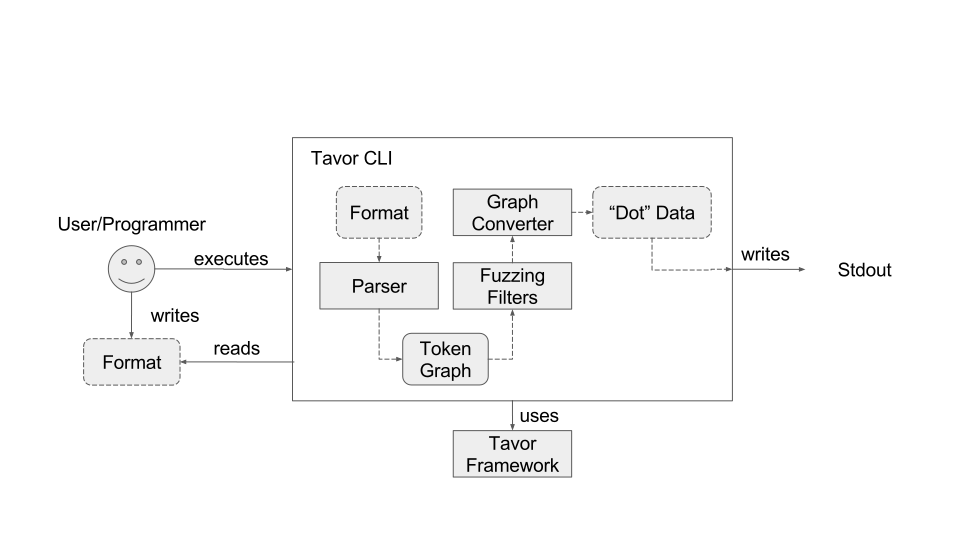
\includegraphics[width=1.0\textwidth]{images/cli-workflow-graph.pdf}
\caption{Workflow for the \texttt{graph} command of the \textsc{Tavor CLI}}
\label{fig:cli-workflow-graph}
\end{figure}

The algorithm for the conversion of the \texttt{token graph} to DOT data is composed by the following two phases:

\begin{listing}[H]
\caption{Convert \texttt{Token Graph} to Simple Graph Structure}
\label{lst:tavor-cli-convert-token-graph}
\begin{gocode}
func buildGraph(token, graph) start, end {
  start, end = {}, {}
  switch type(token) {
    Optional:
      token' = token.Child()
      start', end' = buildGraph(token', graph)

      start.AddOptional(start')
      end.AddOptional(end')
    Concatenation:
      prev = {}
      for i = 0; i < token.NumChildren; i++ {
        token' = token.Child(i)
        start', end' = buildGraph(token', graph)

        graph.AddEdges(prev, start')

        if start'.ContainsOptional() {
          start'.Add(prev)
        }
        prev = start'

        if i == 0 {
          start = start'
        } else if i == token.NumChildren-1 {
          end = end'
        }
      }
    Scope:
      token' = token.Child()
      start' end = buildGraph(token', graph)
    String:
      graph.AddState(token)

      start = {token}
      end = {token}
  }
  return start, end
}
\end{gocode}
\end{listing}

\begin{itemize}
\item Phase one traverses the \emph{token graph} using a recursive depth-first search, which builds upon the assumption, that the used data structure does not contain any loops. As mentioned in Subsection~\ref{subsec:tokens-advanced-concepts}, a loop unrolling step is performed after the format has been parsed to make sure that there are no loops in the token graph. Since each \emph{token type} has its own representation and internal data structure, each type has to be treated differently for the graphical representation using its own implementation. The pseudo code for handling \emph{Optional}, \emph{Concatenation}, \emph{Scope} and \emph{String Tokens} is shown in Listing~\ref{lst:tavor-cli-convert-token-graph}. The traversal function receives the current token to process as well as the graph data structure which needs to be extended. As return values it delivers the set of start and end states of the extended graph data structure.
When traversing an Optional Token, the returned start and end states need to be marked as optional. In case of processing a Concatenation Token, edges need to be added to the graph data structure which connect the individual children of the Concatenation Token. The returned start (resp. end) states are the start (resp. end) states of the first (resp. last) child of the Concatenation Token. When traversing a Scope Token a call to process its only child is performed. Whenever a String Token is processed, a state is added to the resulting graph. As String Tokens are leaves of the token graph no further recursive calls are necessary.
\item Phase two uses the extended graph structure as well as the returned start and end states of phase one to print a DOT representation of the input token graph. End states are depicted using double lines around their label. Optional vertices are shown by using dashed incoming and outgoing arrows. Additional labels and states, which are not included in the pseudo code, are used to depict other tokens such as repeating groups and ranges.
\end{itemize}

The \textsc{Tavor format} in Listing~\ref{lst:tavor-cli-graph-example-tavor} exemplifies how the \texttt{graph} command works. The format results in the DOT data depicted in Listing~\ref{lst:tavor-cli-graph-example-dot} of Appendix~\ref{chapter:AppendixTavorCLI}, which is convertible into the FSM illustrated in Figure~\ref{fig:tavor-cli-graph-example-svg}. All tokens of the format, which are depicted in the graphics as states, are sequential but the tokens $B$ and $F$ are optional, and the group $D E$ is repeated at least twice but at most four times. States are connected using different types of edges, which are depicted as differently styled arrows in the graphics. The FSM depicted in Figure~\ref{fig:tavor-cli-graph-example-svg} starts with the small dot at the top of the graphics. Since $B$ is optional, its incoming and outgoing arrows are dotted. In contrast, the arrow from $A$ to $C$ is solid and is therefore mandatory. However, since $A$ has two outgoing arrows, only one of them has to be taken. Figure~\ref{fig:tavor-cli-graph-example-svg} also illustrates repetition of the $D E$ group, which is indicated by the small dot with an ingoing arrow that has a label with the repetition amount. This arrow causes a loop, therefore marking the repetition. Finally, the accepting state after the repetition has a double bordered circle. Each path of a graph must end in such an accepting state, or else it is not a valid path, i.e., it is not considered by the fuzzing and delta-debugging processes. In this example, it is also possible to go from the accepting state after the repetition to the $F$ token which is optional but also ends in an accepting state.

\begin{figure}[t]
\centering
\begin{minipage}{.5\textwidth}
  \centering
  \begin{listing}[H]
  \caption{Example \textsc{Tavor format} for the \texttt{graph} command}
  \label{lst:tavor-cli-graph-example-tavor}
  \begin{gocode}
  START = A ?(B) C +2,4(D E) ?(F)

  A = "a"
  B = "b"
  C = "c"
  D = "d"
  E = "e"
  F = "f"
  \end{gocode}
  \end{listing}
\end{minipage}%
\begin{minipage}{.5\textwidth}
  \centering
  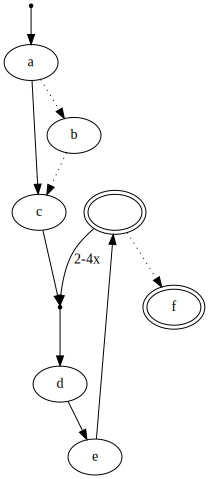
\includegraphics[width=0.5\textwidth]{images/tavor-cli-graph-example.pdf}
  \captionof{figure}{Example graphics for the \texttt{graph} command}
  \label{fig:tavor-cli-graph-example-svg}
\end{minipage}
\end{figure}

\nottitlecapsection{\titlecap{Command }\texttt{fuzz}}
\label{sec:tavor-cli-fuzz}

The \texttt{fuzz} command of the \textsc{Tavor CLI} generates permutations, which conform to a specified format. Additionally, it is capable of forwarding these permutations to external programs, thus allowing to systematically execute a system under test with a stream of inputs for some predefined structure.

Figure~\ref{fig:cli-workflow-fuzz} illustrates the workflow and the interactions of components for the \texttt{fuzz} command. It starts along the same lines as the \texttt{graph} command, by first parsing the \textsc{Tavor format} file into a \texttt{token graph} and by applying optional \texttt{fuzzing filters} on that graph. It then proceeds with its fuzzing loop, which uses a specified \texttt{fuzzing strategy} to generate consecutive permutations. These permutations are written either to the file system or the STDOUT file descriptor. External programs may process these permutations and in turn interact with the \textsc{Tavor CLI} using their exit codes or via STDIN.

\begin{figure}[t]
\hspace*{-1cm}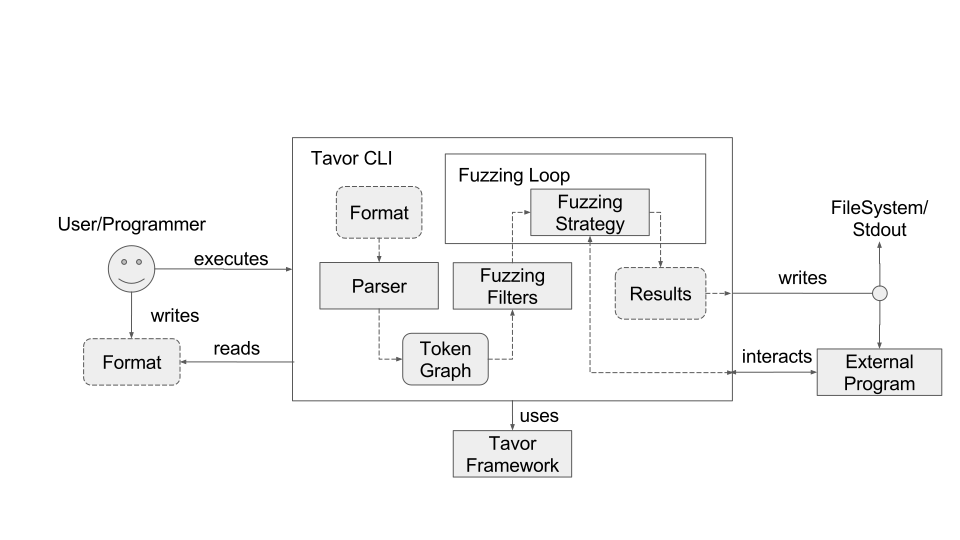
\includegraphics[width=1.1\textwidth]{images/cli-workflow-fuzz.pdf}
\caption{Workflow for the \texttt{fuzz} command of the \textsc{Tavor CLI}}
\label{fig:cli-workflow-fuzz}
\end{figure}

The fuzzing loop of the \texttt{fuzz} command is highly configurable via command line options, which are listed in Listing~\ref{lst:tavor-cli-fuzz-options} of Appendix~\ref{chapter:AppendixTavorCLI}. It may either interact with executables or scripts. When working with executables their exit codes as well as their STDOUT and STDERR file descriptors are processed by the fuzzing loop. In case the \texttt{---exit-on-error} option is set the fuzzing loop will terminate in case an unexpected output is encountered in any of the afore mentioned communication channels. When using scripts the communication with the fuzzing loop is solely performed via STDIN and STDOUT. The fuzzing loop writes permutations separated by a predefined separator to STDIN of the script and waits until the script signals via its STDOUT that it has processed the current permutation. Success or failure, are signaled by using the constants \enquote{Yes} and \enquote{No}.

\begin{figure}[b]
\hspace*{-1cm}\begin{tabular}{cc}
\subfloat[Direct fuzzing of a program]{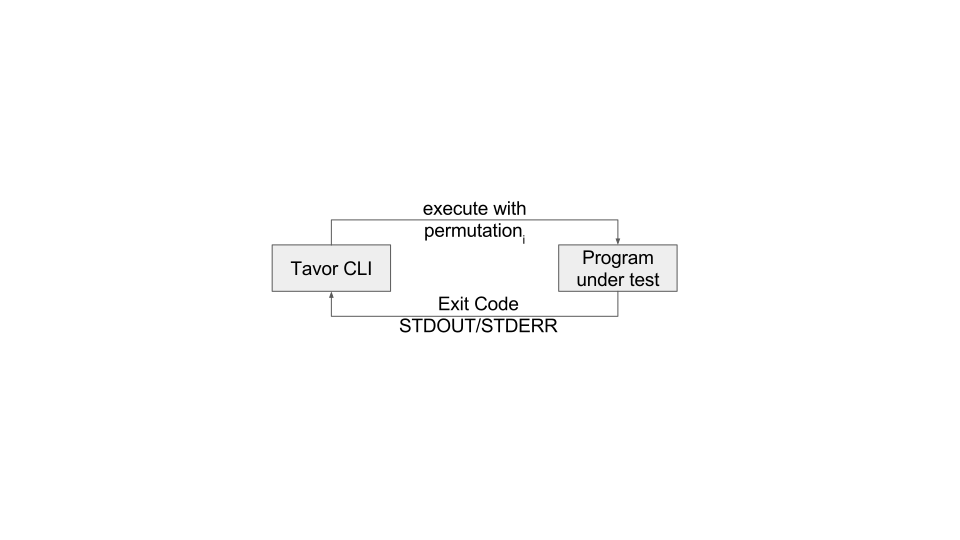
\includegraphics[scale=0.53]{images/cli-fuzz-simple-validation.pdf}\label{fig:cli-fuzz-external-programs-simple}}
\hspace*{0.3cm}\subfloat[Usage of an interposed validation executable]{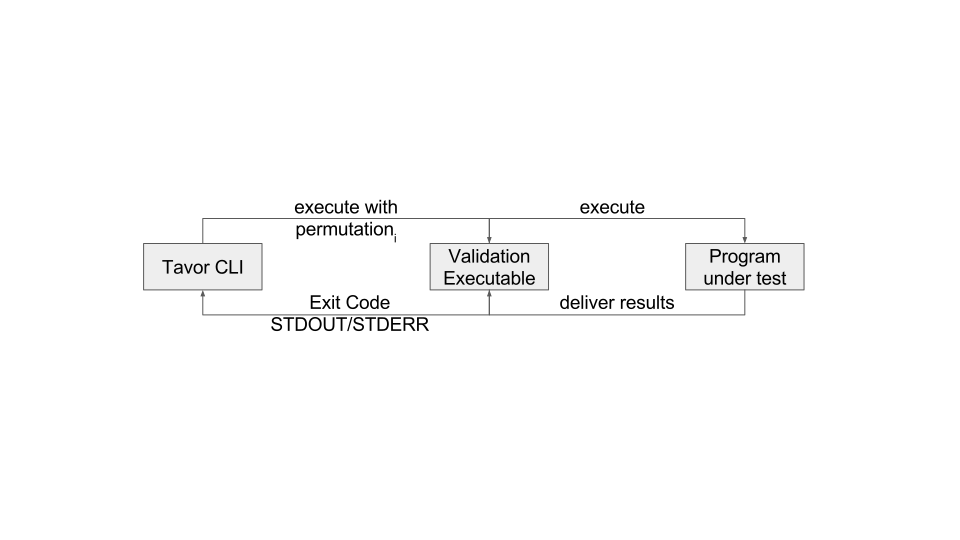
\includegraphics[scale=0.53]{images/cli-fuzz-exec-validator.pdf}\label{fig:cli-fuzz-external-programs-val}}
\end{tabular}
\caption{Fuzzing of external programs}\label{fig:cli-fuzz-external-programs}
\end{figure}

When using the \textsc{Tavor CLI} to immediately fuzz an external program there are two ways to proceed, which are depicted in Figure~\ref{fig:cli-fuzz-external-programs}. Either the program under test is directly passed on to the \textsc{Tavor CLI}, or an interposed validation executable is used. To communicate directly with the program under test has the advantage that only the expected input format is required to start fuzzing. But also has the downside that the built-in validating capabilities of the \textsc{Tavor CLI} are restricted to specifying return codes as well as regular expressions on delivered outputs in STDOUT and STDERR. In case a more thorough validation is required, which cannot be accomplished by the afore mentioned validation capabilities, we advise to use interposed executables or scripts. Consider for instance a program which sorts CSV files by specific columns. An interposed validation function or script could not only check that the program under test exits without errors, but could additionally verify that the output CSV is indeed sorted and its content corresponds to the input CSV file. Several examples of customized scripts and executables are provided at~\footnote{\url{https://github.com/zimmski/tavor/tree/master/examples/fuzzing}}.

\nottitlecapsection{\titlecap{Command }\texttt{validate}}
\label{sec:tavor-cli-validate}

The \texttt{validate} command of the \textsc{Tavor CLI} checks that a given input file conforms to a specified format file. This functionality can be helpful since for instance the \texttt{reduce} command only applies delta-debugging on valid inputs, or in the general case it can be used to examine an input, which was not generated through the given format file.

Figure~\ref{fig:cli-workflow-validate} illustrates the workflow and the interactions of components for the \texttt{validate} command. It starts off by parsing the specified \textsc{Tavor format} file to its corresponding token graph. In the next step this token graph is used to parse the specified input file. In case the input file can be parsed successfully, it conforms to the specified format file. The CLI exits with the exit status $0$ if the input file conforms to the format file, or exits with an exit status unequal to $0$ if it does not conform.

Please refer to Listing~\ref{lst:tavor-cli-validate-options} of Appendix~\ref{chapter:AppendixTavorCLI} for a list of available arguments of the \texttt{validate} command.

\begin{figure}[hb]
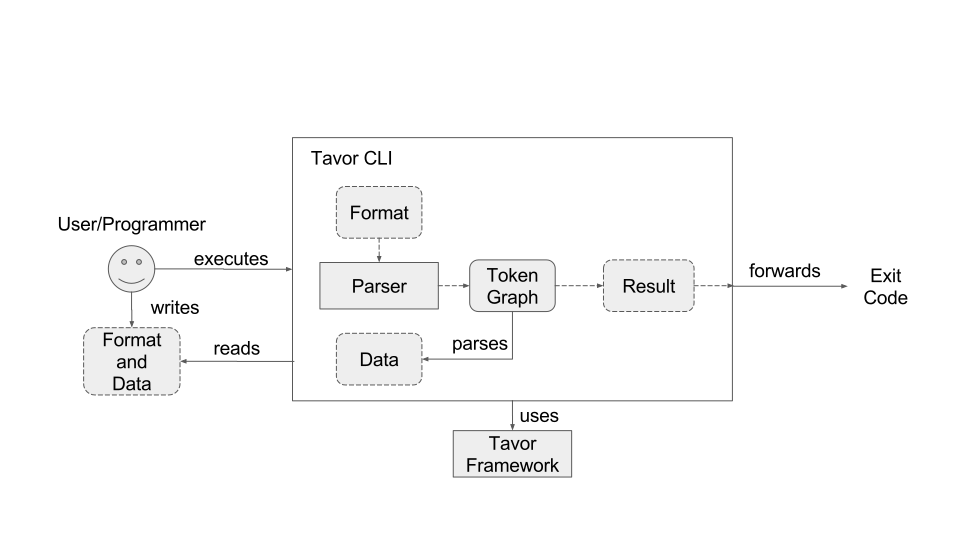
\includegraphics[width=1.0\textwidth]{images/cli-workflow-validate.pdf}
\caption{Workflow for the \texttt{validate} command of the \textsc{Tavor CLI}}
\label{fig:cli-workflow-validate}
\end{figure}


\nottitlecapsection{\titlecap{Command }\texttt{reduce}}
\label{sec:tavor-cli-reduce}

The \texttt{reduce} command applies delta-debugging to a given input according to a specified \textsc{Tavor format} file, i.e., given an input which results in certain program behavior, this capability may be used to systematically reduce the given input while preserving the same behavior.

Figure~\ref{fig:cli-workflow-reduce} depicts the workflow and the interactions of components for the \texttt{reduce} command. It starts similar to the \texttt{validate} command by first parsing the \textsc{Tavor format} file to its associated token graph. This graph is then used to parse the given input data, i.e., the initial input needs to correspond to the specified format. Next, the reduction loop starts by feeding the initial input data to an external resource and capturing its responses. These initial responses are consecutively used by the reduction loop to guide the generation of reduced inputs, i.e., only reductions resulting in these responses are investigated for further reductions.

\begin{figure}[hb]
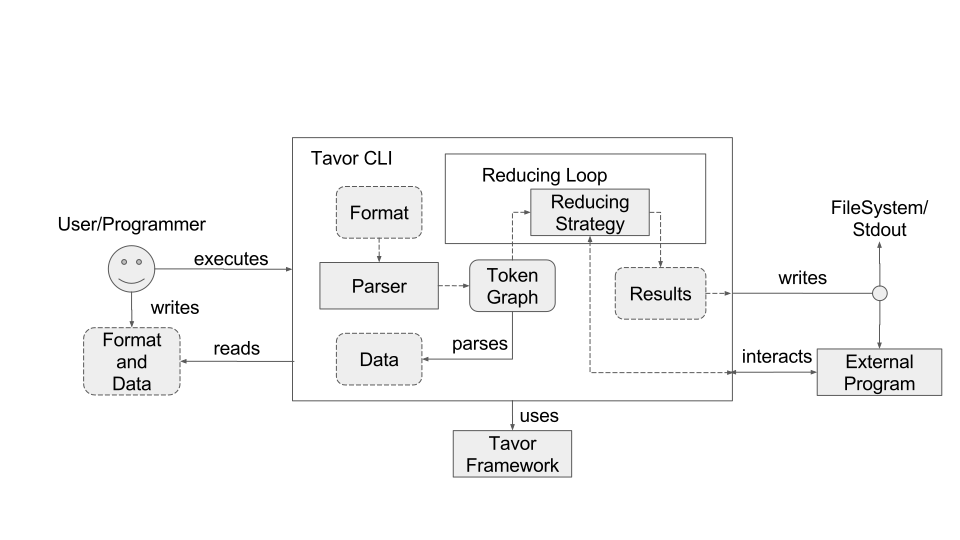
\includegraphics[width=1\textwidth]{images/cli-workflow-reduce.pdf}
\caption{Workflow for the \texttt{reduce} command of the \textsc{Tavor CLI}}
\label{fig:cli-workflow-reduce}
\end{figure}

Various options are available for the \texttt{reduce} command, which are listed in Listing~\ref{lst:tavor-cli-reduce-options} of Appendix~\ref{chapter:AppendixTavorCLI}. The \texttt{reduce} command works along the same lines as the \texttt{fuzz} command, i.e., it may interact with scripts or executables using exit codes as well as STDERR, STDOUT and STDIN as communication channels. Options such as \texttt{---exec-match-stderr} allow to define the expected structure of outputs written to those channels. Please refer to~\footnote{\url{https://github.com/zimmski/tavor/tree/master/examples/deltadebugging}} for example scripts and executables for performing delta-debugging.

\begin{listing}[H]
\caption{Delta-debugging pseudo code for scripts}
\label{lst:tavor-cli-delta-debug-scripts}
\begin{gocode}
func deltaDebugScript(tokenGraph, reduceStrategy) {
  continue, feedback = reduceStrategy(tokenGraph)

  for i = range continue {
    stdin.Write(tokenGraph.String())
    stdin.Write(inputSeparator)

    result = stdout.ReadLine()
    switch result {
      case "YES\n":
        feedback <- Good
      case "NO\n":
        feedback <- Bad
    }

    continue <- i
  }
}
\end{gocode}
\end{listing}

Consider Listing~\ref{lst:tavor-cli-delta-debug-scripts}, which outlines the pseudo code of the reduction loop when working with scripts. A token graph, which holds the parsed input data, as well as the reducing strategy, for reducing the input data, are passed on to function~\texttt{deltaDebugScript}. The reducing strategy receives in Line~2 the token graph to operate on, and returns two channels. In order to communicate that the current processing step is finished the channel \texttt{continue} is used, i.e., the call in Line~4 blocks until the reducing strategy has produced another permutation. The channel \texttt{feedback} is used to signal whether the current permutation still triggers the expected behavior, thus steering the reducing strategy.

\chapter{The \textsc{go-mutesting} Framework}
\label{chapter:goMutesting}

This chapter presents \textsc{go-mutesting}, a framework for performing mutation testing on source code of the programming language \textsc{Go}. Its main purpose is to find source code, which is not covered by any tests. The implementation of \textsc{go-mutesting} with all its assets has been open sourced and is freely available at~\cite{2017_go-mutesting_repository}.

\section{Motivation}
\label{sec:goMutestingMotivation}

The generation of test suites for existing software systems is a major use case of \textsc{Tavor}. One way of evaluating the quality of these test suites is to use mutation testing~\cite{jia2011analysis}, i.e., the software under test gets modified and the generated test suite is verified by checking whether at least one test case fails and therefore if it catches the modifications. A more thorough description of mutation testing can be found in Section~\ref{sec:whatIsMutatinTesting}.

At the time of implementation of \textsc{Tavor}, there has not been any adequate mutation testing tool for the programming language \textsc{Go}. All three existing tools \textsc{manbearpig}~\cite{2017_manbearpig_repository}, \textsc{mutator}~\cite{2017_mutator_repository} and \textsc{Golang-Mutaton-testing}~\cite{2017_Golang-Mutaton-testing_repository} have severe disadvantages:

\begin{itemize}
\item Only one type or even just one case of mutation is implemented.
\item Only one mutation operator can be applied per execution. (\textsc{manbearpig}, \textsc{Golang-Mutaton-testing})
\item The mutation of code is done by directly modifying the characters composing the code. This can lead to lots of invalid mutations, e.g., because of syntax errors. (\textsc{Golang-Mutaton-testing})
\item New mutation operators are not easily implemented and integrated since no common functionality nor API can be utilized.
\item Only one package or file can be analyzed per execution.
\item Other scenarios than \texttt{go test} cannot be applied.
\item Proper cleanup or the handling of fatal failures is not implemented.
\item No automatic tests exist to ensure that the algorithms are working at all.
\item Another language than \textsc{Go} is used for the implementation and it is therefore not possible to utilize the up-to-date language parser. (\textsc{Golang-Mutaton-testing})
\end{itemize}

Due to these insufficiencies we created the \textsc{go-mutesting} framework, which as described in the following sections, overcomes all highlighted disadvantages.

\section{Components}
\label{sec:goMutestingComponents}

\begin{figure}[t]
\hspace*{-1.5cm}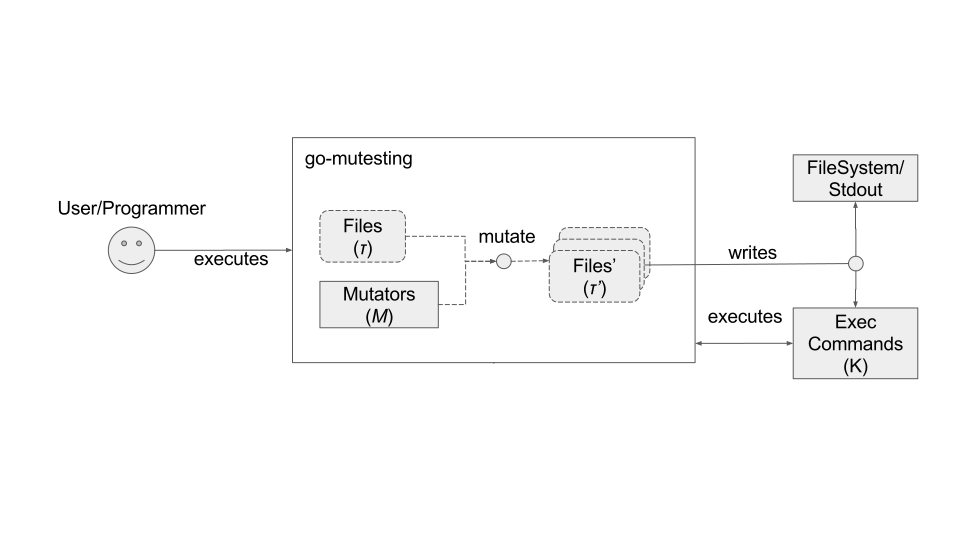
\includegraphics[width=1.1\textwidth]{images/go-mutesting-architecture.pdf}
\caption{Architecture of \textsc{go-mutesting}}
\label{fig:goMutestingArchitecture}
\end{figure}

Figure~\ref{fig:goMutestingArchitecture} depicts the main components of the \textsc{go-mutesting} framework. The user defines a set of files $\tau$ which should be mutated, and optionally a set of \texttt{exec commands} $\kappa$ which should be executed for each modification. Such modifications during mutation testing are called mutants. The framework applies its individual mutation operators called mutators $\mu$ on each file $\tau$, resulting in a set of mutated files $\tau'$ for each mutator-file pair. Each mutated file $\tau'$ is then written to the file system and executing the individual \texttt{exec commands} $\kappa$. After these executions are finished the framework prints the total number of mutants, the number of passing mutants and each failing mutant with their associated source code patches. We consider a mutant to pass in case the test suite failed for its mutation, which means that the mutant has therefore been killed.

Additional to the statistical output of mutants, \textsc{go-mutesting} calculates and outputs the mutation score. Which is a metric on how many mutants have been killed by the test suite and therefore states the quality of the test suite. The mutation score is calculated by dividing the number of passed mutants by the number of total mutants. If we had for example a total of eight mutants, where six are passing then the mutation score would be $6 / 8 = 0.75$. A score of $1.0$, which is most desirable, means that all mutants have been killed.

\section{Mutators}
\label{sec:goMutestingMutators}

The mutation operators of the \textsc{go-mutesting} framework are called mutators, and are used to introduce small deltas into the source files at hand. Mutators operate directly on the AST of a file and must offer two kinds of operations:
\begin{itemize}
\item The \texttt{Change} operation adapts the AST node at hand.
\item The \texttt{Reset} operation restores the original AST node.
\end{itemize}

Working directly on the AST has the advantage, that the introduced mutations are syntactical valid, i.e., compilable source code. Currently the following mutators are supported by the framework:

\begin{itemize}
\item The \texttt{if}-mutator replaces the body of an if-branch with a NOOP statement, which creates an empty usage for every identifier of the substituted body. This is necessary, since the programming language \textsc{Go} marks unused identifiers as syntactical errors.
\item The \texttt{else}-mutator replaces the body of an else-branch with a NOOP statement.
\item The \texttt{case}-mutator replaces the body of a case-clause with a NOOP statement.
\item The \texttt{remove-expression}-mutator modifies the binary logical operators \texttt{AND} and \texttt{OR}. The \texttt{AND} operator is mutated by replacing its left and right operands with the constant \texttt{true}. The \texttt{OR} operator is dealt with along the same lines by using the constant \texttt{false}. For instance, the binary logical expression \texttt{var1 \&\& var2} results in the two mutations \texttt{true \&\& var2} and \texttt{var1 \&\& true}.
\item The \texttt{remove-statement}-mutator modifies statements, such as assignments and the increment/decrement statement, by replacing them with a NOOP statement.
\end{itemize}

The above list of available mutators can easily be extended. A new mutator simply needs to provide the two mutation operations \texttt{Change} and \texttt{Reset}. Additionally, each mutator needs to be registered with the mutator registry of \textsc{go-mutesting} in order to be applied during mutation testing.

\section{Exec Commands}
\label{sec:goMutestingExecCommands}

\texttt{Exec commands} are used by \textsc{go-mutesting} to define the actions which should be taken for each individual mutant. Consider for instance a package with the following files: \texttt{LinkedList.go} and \texttt{LinkedList\_test.go}, where \texttt{LinkedList.go} is a linked list implementation and \texttt{LinkedList\_test.go} is the corresponding file for its tests. For each mutant that \textsc{go-mutesting} produces for the file \texttt{LinkedList.go}, a temporary file with the modifications of the mutant is written. Afterwards the specified \texttt{exec command} is called, executing the tests within \texttt{LinkedList\_test.go}.

A built-in \texttt{exec command} is provided by \textsc{go-mutesting}, which implements the following behavior:

\begin{enumerate}
\item Temporarily overwrite the original file, in our example \texttt{LinkedList.go}, with its mutated content.
\item Execute all tests of the package under test, which are in our example located in \texttt{LinkedList\_test.go}.
\item Restore the original file.
\item Report whether the mutant has been successfully killed.
\end{enumerate}

Customized \texttt{exec commands} can be specified as command line parameters of \textsc{go-mutesting}. Environment variables such as \texttt{MUTATE\_CHANGED} and \texttt{MUTATE\_ORIGINAL} are used to communicate the path of the original as well as the mutated file to the \texttt{exec command}. In order to report success or failure, the following exit codes need to be used by \texttt{exec commands}:
\begin{itemize}
\item Exit code 0 indicates that the mutant was killed, i.e., that the test led to a failed test after the mutation was applied.
\item Exit code 1 indicates that the mutant is alive, i.e., that this could be a flaw in the test suite or even in the implementation.
\item Exit code 2 indicates that the mutant was skipped, since other problems have been found such as compilation errors.
\item An exit code greater than 2 indicates that the mutant produced an unknown exit code, which might be a flaw in the \texttt{exec command}.
\end{itemize}

Two examples of customized \texttt{exec commands} are provided by \textsc{go-mutesting} at~\footnote{\url{https://github.com/zimmski/go-mutesting/tree/master/scripts/exec}}: \texttt{test-current-directory.sh} may be used to execute all tests of the current directory and \texttt{test-mutated-package.sh} to execute all tests originating from the specified package.

\chapter{Evaluation}
\label{chapter:evaluation}

The evaluation performed in the context of this thesis is threefold: First we present a case study, which demonstrates the major capabilities of the \textsc{Tavor framework} and how the framework can be applied to software programs using the example of a coin vending machine. Next we evaluate the generic fuzzing capabilities of \textsc{Tavor} by comparing it with \emph{aigfuzz}~\cite{2017_aig_fuzz}, a dedicated fuzzer for the \emph{AIGER} formats~\cite{biere2007aiger}. Finally we fuzz the JSON format and compare these generations with the manually written test suite of \textsc{Go}'s JSON package.

\section{Case Study: Coin Vending Machine}
\label{sec:evaluationCoinVendingMachine}

A \emph{coin vending machine} is the typical example for showcasing the practicality of model-based testing. In this section we introduce such a coin vending machine to give a step-by-step guide to the techniques presented in this thesis and to show how they can be applied to real world applications. The example is intentionally kept simple so that the basic functionality of each technique can be demonstrated. Source code that is not relevant for the demonstration but necessary for completeness can be found in \textsc{Tavor}'s \enquote{A Complete Example} documentation~\cite{2017_tavor-complete-example}.

The description of the demonstration is divided into the following subsections:

\begin{itemize}
\item Subsection~\ref{subsec:coinVendingMachineDefinition} defines our use-case of the coin vending machine and its implementation.
\item Subsection~\ref{subsec:coinVendingMachineKeywordDriven} defines the keyword-driven testing approach for defining test cases and to test the implementation.
\item Subsection~\ref{subsec:coinVendingMachineFormat} defines our test cases using the \textsc{Tavor Format}, and generates and executes a test suite using the \texttt{fuzz} command of \textsc{Tavor}.
\item Subsection~\ref{subsec:coinVendingMachineMutationTesting} executes the generated test suite and identifies missing test cases by applying code coverage metrics and \textsc{go-mutesting}.
\item Subsection~\ref{subsec:coinVendingMachineMutationDeltaDebugging} introduces some intentional bugs and reduces failing test cases that trigger these bugs using the \texttt{reduce} command of \textsc{Tavor}.
\end{itemize}

\subsection{Definition of the Coin Vending Machine}
\label{subsec:coinVendingMachineDefinition}

In this case study we consider a basic coin vending machine, which accepts coins of two different kinds: \texttt{coin25} and \texttt{coin50} representing credits of value 25 and 50. The coin vending machine keeps track of the currently accepted credit and vends if a credit of 100 is reached. One option to model this behavior, using a finite state machine, is shown in Figure~\ref{fig:coinVendingMachine}. Please note, that the given state machine could be defined more efficiently using state variables commonly used in model-based testing. While the \textsc{Tavor framework} supports such state variables, the \textsc{Tavor format} does not yet fully implement them. One possible direction of future work are such advancements of the \textsc{Tavor format}. Please refer to Chapter~\ref{sec:futureWork} for more details on proposed future extensions.

\begin{figure}[t]
\hspace*{-1.5cm}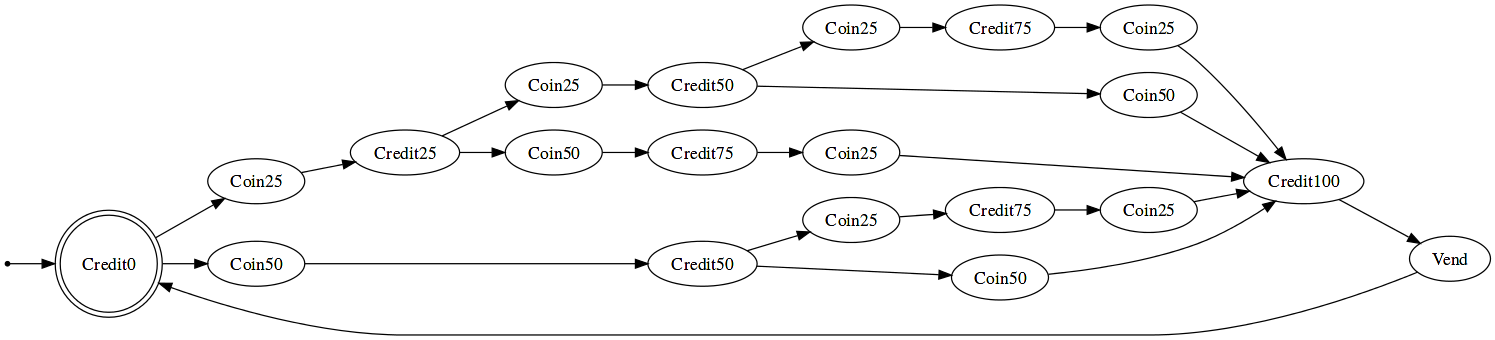
\includegraphics[width=1.1\textwidth]{images/evaluation-coin-vending.png}
\caption{Example Automaton of the Coin Vending Machine}
\label{fig:coinVendingMachine}
\end{figure}

In order to test the coin vending machine of our case study, an approach called keyword-driven testing is applied, which is explored in the next section.

\subsection{Keyword-Driven Testing}
\label{subsec:coinVendingMachineKeywordDriven}

The software testing technique \emph{keyword-driven testing}, introduced by Fewster et al.~in~\cite{fewster1999software}, also known as table-driven testing or action word based testing, separates the documentation of a test case from its implementation. Usually a sequence of keywords is used to specify the course of a test case, i.e., the sequence of keywords \texttt{Credit0, Coin50, Credit50, Coin50, Credit100, Vend, Credit0} specifies a sequence of actions to be executed for testing the coin vending machine. The implementation of the individual actions for each keyword, such as \texttt{Coin50}, is separated from the test case. Thus, making it possible to write test cases without any programming knowledge.

In order to apply keyword-driven testing a format needs to be defined, which specifies the structure of a keyword-driven test case. A test case can then be saved into a single file called a \emph{keyword-driven file}. Additionally, an executor is needed, which maps the individual keywords of such tests to concrete actions.

The \textsc{Tavor framework} offers the package \texttt{keydriven}, which provides various functionality to effectively apply keyword-driven testing. The function \texttt{ReadKeyDrivenFile} is used to parse a keyword-driven file and the type \texttt{Executor} is used to map keywords to their actions. Please consider Listing~\ref{lst:package-key-driven}, which outlines the most important types and functions of package \texttt{keydriven}. Next, we use this functionality to define an executor for the coin vending machine, whose interface is shown in Listing~\ref{lst:vending-machine-interface}. The interface of coin vending machine offers the functions \texttt{Credit}, \texttt{Coin} and \texttt{Vend}. For testing such a machine we introduce three keywords for our keyword-driven files with the following semantics: The keyword \texttt{credit} is used for validating the credit amount currently held by the vending machine, the keyword \texttt{coin} triggers the action of inserting a coin into the vending machine and finally the keyword \texttt{vend} invokes the vending action. Please note, that the keywords \texttt{coin} and \texttt{credit} need integer arguments specifying the coin credit amount.

\begin{listing}
\caption{Functionality of package \texttt{keydriven}}
\label{lst:package-key-driven}
\begin{gocode}
// ReadKeyDrivenFile reads in a keyword-driven file.
func ReadKeyDrivenFile(file string) ([]Command, error)

type Executor interface {
    // Register adds a given key-action pair to the executor.
    Register(key string, action Action) error
    // Execute executes a set of keyword-driven commands.
    Execute(cmds []Command)
}

// NewExecutor initializes and returns a new executor.
func NewExecutor() *Executor
\end{gocode}
\end{listing}

\begin{listing}
\caption{Interface of the Coin Vending Machine Module}
\label{lst:vending-machine-interface}
\begin{gocode}
type VendingMachine interface {
    // Credit returns the current credit of the coin vending machine.
    Credit() int
    // Coin inserts a coin into the coin vending machine and increases its credit.
    Coin(credit int) error
    // Vend executes a vend of the machine if enough credit (100) was put in and returns true.
    Vend() bool
}
\end{gocode}
\end{listing}

The executor connects the keyword-driven files, each representing a test scenario, with the implementation under test. It reads, parses and validates keyword-driven files, executes sequentially each key with its arguments by invoking actions of the implementation and validates these actions. A test passes if each action executes without any problems. The pseudocode for an executor for the coin vending machines of the case study is shown in Listing~\ref{lst:vending-machine-executor}. Please note, that the pseudocode does not include any error handling for the keyword-driven files and command line arguments in order to keep the code listing short. The main method subsequently parses the keyword-driven file, initializes the executor and executes the read commands. The actual connection between keywords and actions is made in function \texttt{initExecutor}, which registers for each keyword a callback function using the functionality of the provided package \texttt{keydriven}. Consider for instance the registration of the keyword \texttt{credit}, which includes one parameter denoting the expected amount of credit.\footnote{Validating the presence and type of keyword parameters has awas skipped to keep the pseudocode short.} When this keyword is encountered, the defined expected credit is compared with the currently held credit of the coin vending machine. In case these two values diverge, an error is returned, indicating that the test scenario failed.

\begin{listing}[hb]
\caption{Example Executor for a Coin Vending Machine}
\label{lst:vending-machine-executor}
\begin{gocode}
func main() {
  cmds := keydriven.ReadKeyDrivenFile(os.Args[1])
  executor := initExecutor()
  if err := executor.Execute(cmds); err != nil {
    os.Exit(exitFailed)
  }
  os.Exit(exitPassed)
}

func initExecutor() *keydriven.Executor {
  executor := keydriven.NewExecutor()
  machine := implementation.NewVendingMachine()
  executor.Register("credit", func(key string, parameters ...string) error {
    expected := strconv.Atoi(parameters[0])
    got := machine.Credit()
    if expected != got {
      return fmt.Errorf("Credit should be %d but was %d", expected, got)
    }
    return nil
  })
  executor.Register("coin", func(key string, parameters ...string) error {
    if err := machine.Coin(strconv.Atoi(parameters[0])); err != nil {
      return err
    }
    return nil
  })
  executor.Register("vend", func(key string, parameters ...string) error {
    if vend := machine.Vend(); !vend {
      return fmt.Errorf("Could not vend")
    }
    return nil
  })
  return executor
}
\end{gocode}
\end{listing}

The next step for testing the coin vending machine is to generate keyword-driven files, which is done in the next section by applying \textsc{Tavor's} format and fuzzing capabilities.

\begin{listing}
\caption{\textsc{Tavor Format} for Coin Vending Machine}
\label{lst:tavor-format-coin-vending}
\begin{gocode}
START = Credit0 *(Coin25 Credit25 | Coin50 Credit50)

Credit0  = "credit" "\t" 0 "\n"
Credit25 = "credit" "\t" 25 "\n" (Coin25 Credit50 | Coin50 Credit75)
Credit50 = "credit" "\t" 50 "\n" (Coin25 Credit75 | Coin50 Credit100)
Credit75 = "credit" "\t" 75 "\n" Coin25 Credit100
Credit100 = "credit" "\t" 100 "\n" Vend Credit0

Coin25 = "coin" "\t" 25 "\n"
Coin50 = "coin" "\t" 50 "\n"

Vend = "vend" "\n"
\end{gocode}
\end{listing}

\subsection{\textsc{Tavor Format} and Fuzzing}
\label{subsec:coinVendingMachineFormat}
 A valid keyword-driven file for the \textsc{Tavor framework}  needs to adhere to the following conditions: Each line starts with and holds at most one keyword. Each keyword may be followed by zero, one or more arguments, where each argument is preceded by a tab character. Finally each line ends with the new-line character. Combining the state machine shown in Figure~\ref{fig:coinVendingMachine}, the defined keys and the rules for the keyword-driven format together, results in the \textsc{Tavor format} shown in Listing~\ref{lst:tavor-format-coin-vending}.

This format file can now be easily fuzzed using the \textsc{Tavor} binary, resulting in outputs such as Listing~\ref{lst:key-driven-file-vending-machine}. Since there is a loop in the specified format, the graph can be traversed more than once, resulting in longer keyword-driven files which execute the action \texttt{vend} more than once. The default fuzzing strategy \texttt{Random} can create all possible permutations of a format but since it is random, it will need enough time to do so. Since even random events often lead to choosing the same path in a graph, many duplicated results will be generated using the \texttt{Random} fuzzing strategy. To work around this problem the \texttt{AllPermutations} strategy can be used which, as its name suggests, generates all possible permutations of a graph. This strategy should be used wisely since even small graphs can have an enormous amount of permutations. Also, since the example graph has a loop, we can state that there is an infinite amount of permutations. To work around this additional problem, the \texttt{---max-repeat} argument, which enforces a maximum for traversals and repetitions of loops, is used with a suitable value. Choosing a good value for \texttt{---max-repeat} is challenging, because high values may result in many repetitive permutations that will not improve the testing process. Choosing a small value on the other hand can lead to a bad coverage, which means that some scenarios are not tested.

\begin{listing}
\caption{Key-driven File for the Coin Vending Machine Test Scenario}
\label{lst:key-driven-file-vending-machine}
\begin{textcode}
credit  0
coin    25
credit  25
coin    50
credit  75
coin    25
credit  100
vend
credit  0
\end{textcode}
\end{listing}

The chosen \textsc{Tavor Format} for testing the coin vending machine of this case study is fairly easy to understand as it contains only a single loop. We choose the value $2$ for \texttt{\mbox{---max-repeat}} to ensure that the repetitive part of the state machine is executed at least once. By executing the following command: \texttt{tavor ---format-file vending.tavor ---max-repeat 2 fuzz ---strategy AllPermutations ---result-folder testset ---result-extension ".test"}. A total of 31 keyword-driven files is generated and stored in folder \texttt{testset}. Each written test file is named by \textsc{Tavor} according to its MD5 hash with the specified extension \texttt{.test}.

Since all components for testing the given state machine are now defined the next step is to execute the actual tests using the executor. One option to do this, is by invoking the program of Listing~\ref{lst:vending-machine-executor} for each test file, e.g., \texttt{go run executor.go testset/fba58bb35d28010b61c8004fadcb88a3.test}.

\afterpage{\clearpage}

Executing each keyword-driven file separately is tedious. A better solution would be to extend the executor, but this would also mean more restrictions and more flaw possibilities in the executor code. Alternatively a simple Bash script which executes each keyword-driven file of the folder \texttt{testset} and immediately exits if the execution of a file fails can be used. An example for such a Bash script is shown in Listing~\ref{lst:key-driven-test-script}.

\begin{listing}
\caption{Key-driven Test Script}
\label{lst:key-driven-test-script}
\begin{minted}[
  linenos,
  numbersep=5pt,
  breaklines,
  bgcolor=white,
]{bash}
#!/bin/bash
shopt -s nullglob
for file in testset/*.test
do
  echo "Test $file"
  ./executor $file
  if [ $? -ne 0 ]; then
    echo "Error detected, will exit loop"
    break
  fi
done
\end{minted}
\end{listing}

Executing this script reveals no errors, i.e., all tests passed. In the next section we introduce some defects into the implementation of the coin vending machine and check whether the test suite is able to reveal them.

\subsection{Mutation Testing}
\label{subsec:coinVendingMachineMutationTesting}

Although the test suite introduced in Subsection~\ref{subsec:coinVendingMachineFormat} passes, it is no guarantee that it verifies all functionality of the implementation of the coin vending machine. The first step to determine the quality of the test suite is to look at its code coverage. By converting the given test cases to ordinary \textsc{Go} test cases we can record their code coverage using the command\texttt{go test -coverprofile=coverage.out} followed by the command \texttt{go tool cover -html=coverage.out} to display the coverage information. Using this approach we determined that only three lines are not covered of an overall of 18 coverable lines. These three lines handle two negative cases of the coin vending machine: the first is the insertion of an unknown coin, i.e., an unknown coin amount, and the second is the invocation of the vending action, even though an amount of 100 credits has was reached. Both scenarios are not implemented in our model for generating test cases and are not implemented in the executor. Hence, new keywords would need to be introduced to generate and handle these scenarios. The shown code coverage and our interpretation of the results therefore match our model. However, code coverage only determines that a statement was executed but does not prove that a statement has actuawas verified.

The main purpose of mutation testing is to determine the quality of a test suite at hand by determining whether statements are tested by a given test suite. This technique, as well as \textsc{go-mutesting}, a framework for applying it, was introduced in detail in Chapter~\ref{chapter:goMutesting}. We apply mutation testing on our implementation and test suite by invoking the command \texttt{TESTSET=./testset/ go-mutesting coin}. Please note, that \enquote{./testset/} states the relative path to the directory holding the generated test cases and \enquote{coin} defines the \textsc{Go} package that should be analyzed. The relevant parts of the output for this command can be found in Listing~\ref{lst:mutation-testing-vending-machine} of Appendix~\ref{chapter:coinVendingMachine}. Since the implementation is rather simple, only a small amount of mutations can be applied. A total of five mutations were applied by \textsc{go-mutesting}, of whom three were killed by the generated test suite. This results in a mutation score of $3 / 5 = 0.6$. Investigating the two alive mutations shows the same result as with the code coverage analysis, i.e., only two negative cases are not covered. Hence, the used model to generate test cases applies to all possible positive test scenarios.

The remainder of this section discusses different flaws that can be introduced into the implementation of the coin vending machine, and checks, whether the previously generated test suite catches them. The following defects were introduced separately to the coin vending machine implementation:
\begin{enumerate}
\item \textbf{The \texttt{Coin} method no longer increases the credit:} This flaw can easily be introduced either by removing the addition in the \texttt{Coin} method, or by using a non-pointer type as receiver for the \texttt{Coin} method which leaves the state of the machine untouched.
\item \textbf{The \texttt{Vend} method no longer decreases the credit:} This flaw can be introduced along the same lines as the previous one, by either removing the subtraction in method \texttt{Credit} or by using a non-pointer type as a receiver.
\item \textbf{Every second 25 coin no longer increases the credit:} The defect type "works once but not twice" can be found in many programs. To emulate this kind of defect an additional state member was introduced to the coin vending machine implementation in order to trigger such a defect on every second call of method \texttt{Coin} with value 25.
\end{enumerate}

Please note, that the first two defect types are automatically introduced using \textsc{go-mutesting}. The third defect type on the other hand is not yet supported by the framework and needs to be introduced by hand.

The test suite from Section~\ref{subsec:coinVendingMachineFormat} was executed individually for each of the above flaws. Each defect type was successfully revealed, showcasing that the \textsc{Tavor framework} can be used to generate test suites with little effort, that are able to catch these implementation flaws. Besides its support for fuzzing and keyword-driven testing, the \textsc{Tavor framework} may be also used to apply delta-debugging in order to decrease debugging times. Applying delta-debugging to the coin vending machine case study is the content of the subsequent section.

\subsection{Delta-Debugging}
\label{subsec:coinVendingMachineMutationDeltaDebugging}

Delta-debugging, introduced in Section~\ref{sec:whatIsDeltaDebugging}, is a technique to automatically reduce error revealing inputs in order to make debugging easier for developers. Consider, for instance, a very long keyword-driven file revealing a defect. A developer would need to walk through a very long path through the state machine before she is able to find the cause of the problem. Often not the whole keyword-driven file is necessary to successfully reproduce the problem. When this is the case delta-debugging comes in handy to automatically reduce these keyword-driven files. The final result of the delta-debugging process should be a minimal test case, which still triggers the same defect as the original test case. This can be automatically or semi-automatically done by the \texttt{reduce} command of the \textsc{Tavor} binary. The binary uses our \textsc{Tavor format} file to parse and validate the given keyword-driven file and for reducing its data according to the rules defined by the format file. For instance optional content like repetitions can be reduced to a minimal repetition. In the coin vending machine case study the iterations of the vending loop can be reduced.

When executing test case \texttt{testset/fba58bb35d28010b61c8004fadcb88a3.test},\footnote{This test case was generation in Section~\ref{subsec:coinVendingMachineFormat}.} for the third defect type of Section~\ref{subsec:coinVendingMachineMutationTesting}, then the output in Listing~\ref{lst:key-driven-test-output} is generated. The introduced defect is triggered in the second vending iteration, because every second $25$ coin does not increase the machine's credit counter.

\begin{listing}
\caption{Key-driven Test Output}
\label{lst:key-driven-test-output}
\begin{textcode}
credit [0]
coin [50]
credit [50]
coin [50]
credit [100]
vend []
credit [0]
coin [50]
credit [50]
coin [25]
credit [75]
coin [25]
credit [100]
Error: Credit should be 100 but was 75
\end{textcode}
\end{listing}

First the semi-automatic method of the \textsc{Tavor} \texttt{reduce} command is applied to the test case at hand. The given format file is used to reduce the given input. Every reduction step displays the question "Do the constraints of the original input still hold for this generation?" to the user. The user's task is to inspect and validate the reduced output of the original data and decide by giving feedback if the defect is triggered (\texttt{yes}) or not (\texttt{no}). The following command starts this process: \texttt{tavor --format-file vending.tavor reduce --input-file testset/fba58bb35d28010b61c8004fadcb88a3.test}. Please refer to Listing~\ref{lst:semi-automated-delta-debug-vending-machine} of Appendix~\ref{chapter:coinVendingMachine} for the generated outputs of this command.

Semi-automatic processes can be tedious for big data especially due to the manual validation. The \textsc{Tavor} binary does therefore provide several methods to reduce the given inputs in a fully automated manner. The executor written in Section~\ref{subsec:coinVendingMachineKeywordDriven} was reused for this process. The reduction process is aided by the executor by exiting with different status codes on success or failure. The following command starts the fully automated delta-debugging process: \texttt{tavor --format-file vending.tavor reduce --input-file testset/fba58bb35d28010b61c8004fadcb88a3.test --exec "./executor TAVOR\_DD\_FILE" --exec-argument-type argument --exec-exact-exit-code}. Each exit status code of the executor is compared to the original exit status code. If it is not equal, the reduction process will try an alternative reduction step until a reduction path is found that which leads to the minimum. The output of the execution of this command is shown in Listing~\ref{lst:fully-automated-delta-debugging-output}.

\begin{listing}
\caption{Fully Automated Delta-Debugging for Coin Vending Machine}
\label{lst:fully-automated-delta-debugging-output}
\begin{textcode}
credit  0
coin    50
credit  50
coin    25
credit  75
coin    25
credit  100
vend
credit  0
\end{textcode}
\end{listing}

The fully automated delta-debugging step concludes our case study, which demonstrates the major capabilities of the \textsc{Tavor framework} and how they can be applied to facilitate model-based testing, fuzzing and delta-debugging on software programs.

\afterpage{\clearpage}

\section{Fuzzing the AIGER ASCII format}
\label{sec:evaluationFuzzingAigerAscii}

One of the major claims of the \textsc{Tavor framework} is to be a generic fuzzing tool, i.e., by providing the respective \textsc{Tavor format}, inputs of any format may be fuzzed. To evaluate this claim we compare the generations of \emph{aigfuzz}~\cite{2017_aig_fuzz}, a dedicated fuzzer for the AIGER formats~\cite{biere2007aiger}, with the generations of \textsc{Tavor}. In Subsection~\ref{subsec:evaluationIntroducingAigerAsciiFormat} we shortly introduce the AIGER ASCII format, subsequently Subsection~\ref{subsec:evaluationAigerExperimentalSetup} outlines the details of the experimental setup and finally Subsection~\ref{subsec:evaluationAigerResultsConclusions} presents the results and conclusions we draw from this evaluation.

\subsection{Introducing the AIGER ASCII format}
\label{subsec:evaluationIntroducingAigerAsciiFormat}

The AIGER ASCII format is used to model and-inverter graphs, containing inputs, outputs, latches, and-gates and inverters. We will discuss the structure and constraints of this format using its \textsc{Tavor format} definition shown in Listings~\ref{lst:tavor-aiger-ascii-format-1} and~\ref{lst:tavor-aiger-ascii-format-2}.\footnote{Please note, that the \textsc{Tavor format} definition was split up into two listings due to its length.}

\begin{listing}[H]
\caption{\textsc{Tavor format} denoting the AIGER ASCII format part one}
\label{lst:tavor-aiger-ascii-format-1}
\begin{minted}[
  mathescape,
  linenos,
  numbersep=5pt,
  breaklines,
  bgcolor=white,
]{go}
$Variable Sequence = start: 2,
                     step: 2
ExistingLiteral = 0, // false
                | 1, // true
                | $Variable.Existing,
                | ${Variable.Existing + 1} // +1 means a NOT for this input
Inputs = *(Input)
Input = $Variable.Next "\n"
Latches = *(Latch)
Latch = $Variable.Next " " ExistingLiteral "\n"
Outputs = *(Output)
Output = ExistingLiteral "\n"
ExistingLiteralAnd = 0, // false
                   | 1, // true
                   | ${Variable.Existing not in (AndCycle)},
                   | ${Variable.Existing not in (AndCycle) + 1} // +1 means a NOT for this input

// AndCycle finds all paths beginning from the variable andLiteral
AndCycle = ${andList.Reference path from (andLiteral) over (e.Item(0)) connect by (e.Item(2) / 2 * 2, e.Item(4) / 2 * 2) without (0, 1)}
Ands = *(And)
And = $Variable.Next<andLiteral> " " ExistingLiteralAnd " " ExistingLiteralAnd "\n"

Header = "aag ",
         (,                                                  // M
           ${Inputs.Count + Latches.Count + Ands.Count},
         | ${Inputs.Count + Latches.Count + Ands.Count + 1}, // M does not have to be exactly I + L + A there can be unused Literals
         ) " ",
         $Inputs.Count " ",                                  // I
         $Latches.Count " " ,                                // L
         $Outputs.Count " ",                                 // O
         $Ands.Count "\n"                                    // A
\end{minted}
\end{listing}

\begin{listing}
\caption{\textsc{Tavor format} denoting the AIGER ASCII format part two}
\label{lst:tavor-aiger-ascii-format-2}
\begin{minted}[
  mathescape,
  linenos,
  numbersep=5pt,
  breaklines,
  bgcolor=white,
]{go}
Body = Inputs,
       Latches,
       Outputs,
       Ands<andList>

Comments = "c\n",
           *(Comment)
Comment = *([\w ]) "\n"

Symbols = +0,$Inputs.Count(SymbolInput),
          +0,$Latches.Count(SymbolLatch),
          +0,$Outputs.Count(SymbolOutput)

SymbolInput = "i" $Inputs.Unique<=e> $e.Index " " +([\w ]) "\n"
SymbolLatch = "l" $Latches.Unique<=e> $e.Index " " +([\w ]) "\n"
SymbolOutput = "o" $Outputs.Unique<=e> $e.Index " " +([\w ]) "\n"

START = $Variable.Reset,
        Header,
        Body,
        ?(Symbols),
        ?(Comments)
\end{minted}
\end{listing}

Variables in the AIGER ASCII format are indexed using positive even integer values greater or equal to two, this coherence is modeled by using a sequence in the token \texttt{Variable}. Inverters in the AIGER ASCII format are denoted by setting the least significant bit of a literal, due to this reason only even integers are used for variables. Let us assume literal $2$ denotes an input to the and-inverter graph, then the literal $3$ is used to denote the negation of this input. All existing literals for the and-inverter graph are defined in token \texttt{ExistingLiteral}. The constants \texttt{TRUE} and \texttt{FALSE} are denoted using the literals $0$ and $1$. Additionally, all variables and their negations are part of all available existing literals.

The inputs and outputs of the and-inverter graph are represented by a single valid variable. A latch is defined by first listing its current state followed by its next state separated by a whitespace character. The AIGER ASCII format poses by far the most constraints on used and-gates. An and-gate is defined by first listing its left-hand side literal followed by its two right-hand side literals each separated by whitespace characters, e.g., for storing the result of the AND operation on the two variables 2 and 4 in variable 6 one would need to write \texttt{6 2 4}. This coherence is captured by token \texttt{And}. The AIGER ASCII format allows the connection of several and-gates, i.e., the left-hand side literal of an and-gate, or its negation, may be used in the right-hand side literal of another and-gate. However, it is prohibited to model cycles of and-gates in the and-inverter graph. Hence, the tokens \texttt{ExistingLiteralAnd} and \texttt{AndCycle} are necessary to ensure no cycles are generated by \textsc{Tavor}.

The header of the AIGER ASCII format starts with the string \texttt{aag} followed by five integers \texttt{M I L O A} separated by whitespace characters. Where \texttt{M} denotes the number of variables, \texttt{I} the number of inputs, \texttt{L} the number of latches, \texttt{O} the number of outputs and \texttt{A} the number of and-gates. The header is followed by the body of the format, listing consecutively the definitions of inputs, latches outputs and and-gates. The body is succeeded by an optional symbol table and an optional comment section. A symbol table is used to connect symbols, which are ASCII strings, to specific inputs, outputs or latches. Please note, that at most one symbol can be connected to a specific variable. In order to connect the first input with symbol \texttt{my\_input} we need to denote \texttt{i0 my\_input}. For more details on the constraints and structure of the AIGER ASCII format, please refer to~\cite{biere2007aiger}.

During the conduction of this evaluation we observed, that while it is possible to represent the AIGER ASCII format with the \textsc{Tavor framework}, it is a challenging task to come up with the correct format definition and semantics. Of course, it is still more time consuming to write a dedicated AIGER ASCII format fuzzer than defining its \textsc{Tavor format}, since a lot of boilerplate code and algorithms have to be created to handle the fuzzing part of the defined structures. Additionally, data structures as well as the architecture of such a dedicated fuzzer have to be defined and implemented instead of simply defining the syntax and semantics of a format, as can be done using the \textsc{Tavor format}. In the next subsections we will compare the generations of \textsc{Tavor} using the format defined in this subsection with the generations of the \emph{aigfuzz} fuzzer.

\subsection{Experimental Setup}
\label{subsec:evaluationAigerExperimentalSetup}

This subsection describes the experimental setup of this evaluation in detail. First we describe the hardware of the evaluation, then we outline how the test sets were generated and finally we describe the compilation and execution details.

\textbf{Hardware}\\
The generation of the test sets as well as their compilation and execution, have been executed in a KVM VM with OpenSUSE 42.3 as the hypervisor and guest operating system. The VM consisted of 4 virtual cores of an Intel Xeon CPU E3-1275 v5 with 3.60GHz, 16GB of DDR4 ECC RAM with a clock frequency of 2400 MHz and a dedicated volume to two Toshiba XG3 M.2 NVMe drives in a software RAID1 configuration.

\textbf{Test Set Generation}\\
In order to compare the generations of \emph{aigfuzz} with the generations of the \textsc{Tavor framework}, three different test sets were created. The first test set was generated using the command \texttt{aigfuzz -a}, in order to generate only AIGER ASCII format files using the aigfuzz tool. The remaining two test sets were created with the \textsc{Tavor framework} using the format introduced in Listings~\ref{lst:tavor-aiger-ascii-format-1} and~\ref{lst:tavor-aiger-ascii-format-2}. One is generated using the \emph{random} fuzzing strategy, where the parameter defining the maximum number of loop unrollings \texttt{max-repeat} is set to \texttt{10}, in order to ensure that also large files are being generated. The other test set is generated using the \emph{AlmostAllPermutations} fuzzing strategy, with \texttt{max-repeat} set to \texttt{1}\footnote{Higher values for \texttt{max-repeat} are currently not supported for the AIGER format in combination with the \emph{AlmostAllPermutations} fuzzing strategy due to an error in the generation of permutations.}.

For the randomly generated test sets a maximum of unique 10.000 test cases were generated. And for the \emph{AlmostAllPermutations} test set of \textsc{Tavor} all tests were created, i.e., 204 tests. Please note, that the number of possible tests for this fuzzing strategy is finite as it is bounded through the definition of \texttt{max-repeat}. Each of the generated test sets is stored in its own folder, where each generated file is stored named by its MD5 checksum using the file extension \texttt{.test}, e.g., \texttt{b6fe6a6049c39ab112f778769e92cc76.test}.

\textbf{Compilation and Execution}\\
The comparison of the three test sets is performed by measuring the code coverage they reach in the AIGER toolset, which provides various executables operating on AIGER ASCII files. For this experiment we used the AIGER toolset in version 1.9.4. from \url{http://fmv.jku.at/aiger/}.

In order to compile the toolset, we first created the default \texttt{Makefile} of the toolset by running \texttt{./configure}. Next this \texttt{Makefile} has been adapted to do compilations using Clang in version 4.0.1., by setting \texttt{CC=clang-4.0.1}. Additionally, we changed the environment variable \texttt{CFLAGS} to \texttt{-O3 -DNDEBUG -fprofile-instr-generate -fcoverage-mapping} to make the coverage information for each execution available, and the address sanitizer option \texttt{-fsanitize=address} was appended to \texttt{CFLAGS}, enabling the detection and reporting of memory errors during runtime. Finally we ran \texttt{make} to compile all binaries of the toolset with the defined configuration.

The LLVM developer tools were used to make the coverage information for this evaluation available. To run for instance the \texttt{aigand} tool on test case \texttt{12666cece4dbf5bfc1e1d46c02819da} of the \texttt{Random} fuzzing strategy the following command needs to be executed: \texttt{LLVM\_PROFILE\_FILE=./aiger/outa.profraw ./aiger/aigand ./aiger/tavor-random/12666cece4dbf5bfc1e1d46c02819da.test}. This command stores the coverage information of this execution in file \texttt{./aiger/outa.profraw}. Before this file can be used, it needs to be indexed using the following command \texttt{llvm-profdata merge -sparse outa.profraw -o outa.profdata}.

Figure~\ref{fig:code-coverage} depicts the relevant data which has been gathered for a single run. Code regions may span multiple lines, i.e., for blocks without any control flow. But it is also possible that a single line contains several regions, e.g., in \texttt{if(a || b)}. Lines inform about the lines of code that have been covered. Please refer to~\cite{2017_llvm_code_coverage}, for a detailed description of the used coverage tool and its workflows.

\begin{figure}[t]
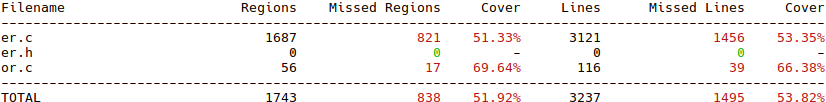
\includegraphics[width=\textwidth]{images/evaluation-code-coverage.png}
\caption{Code Coverage Example}
\label{fig:code-coverage}
\end{figure}

Since we run each test case separately per tool, we need to merge the code coverages for the individual runs in order to gain the cumulative coverage of a test set. To merge two code coverages the following command was executed: \texttt{llvm-profdata merge -sparse foo1.profraw foo2.profdata -o foo3.profdata}.

For automatically running each generated test on the tools of the AIGER toolset and computing their cumulative coverage per test set, a \textsc{Go} script has been devised. The pseudocode outlining the contents of this script is shown in Listing~\ref{lst:evaluation-script}. It iterates over the three test sets and cleans up their execution directory using the auxiliary function \texttt{cleanupExecutionDirectory}. For each of the AIGER tools used for this evaluation the tests of a test set are executed using the auxiliary function \texttt{execute}, which returns the coverage \texttt{c} as well as exit status \texttt{e} of the execution. These code coverages and exit states are stored and cumulated per tool and test set. Finally, the results of the evaluation are printed out for examination.

\begin{listing}
\caption{Pseudo Code for the Script for performing the AIGER Evaluation}
\label{lst:evaluation-script}
\begin{gocode}
testSets := [...]string{"aigFuzz -a", "tavarRandom", "tavorAllPerms"}
tools := [...]string{"aigand", "aigbmc -m", "aigflip", "aiginfo", ...}

for _, ts := range testSets {
  cleanupExecutionDirectory(ts)
  for _, tool := range tools {
    for _, t := range testsOfTestSet(ts) {
      c, e := execute(tool, t)

      cumulateCoverage(ts, tool, c)
      cumulateExitStatus(ts, tool, e)

      cleanup(t)
    }
  }
}

printResults()
\end{gocode}
\end{listing}

\subsection{Results and Conclusions}
\label{subsec:evaluationAigerResultsConclusions}

The statistic of the generated test sets is presented in Table~\ref{table:evaluationAIGERGeneration}, where column \texttt{Name} denotes the name of the test set using the naming convention <tool>-<fuzzing strategy>, \texttt{Cases} holds the number of unique tests in the test set, \texttt{Invalid} informs about the number of invalid generations, i.e., those not conforming to the format specification, \texttt{Size(MB)} holds the required disk space of the test set in megabytes and \texttt{Time(s)} informs about the time needed to generate the test set using the respective tool in seconds. When comparing the test set \texttt{aigfuzz-random} with \texttt{tavor-random} we observe that \textsc{Tavor}'s generation is almost twice as fast as the generation of \emph{aigfuzz}, which may be a result of the generated test set size. The tests generated by \emph{aigfuzz} are 3.5 times larger than the ones generated by \textsc{Tavor}. Additionally, \textsc{Tavor} generated 918 invalid tests which has not been done on purpose. Hence, either the format specification or the \textsc{Tavor framework} contains a bug. By far the smallest test set, with 204 tests, is represented by \texttt{tavor-aap}, which has been generated with the \emph{AlmostAllPermutations} fuzzing strategy.

\begin{table}
\caption{Comparison of the Test Set Generation of the AIGER Evaluation}
\label{table:evaluationAIGERGeneration}
\center
\begin{tabular}{| l | l | l | l | l |}
\hline \textbf{Name} & \textbf{Cases} & \textbf{Invalid} & \textbf{Size(MB)} & \textbf{Time(s)} \tabularnewline
\hline \emph{aigfuzz-random} & 10000 & 0 & 1125 & 143.90 \tabularnewline
\hline \emph{tavor-random} & 10000 & 918 & 40 & 82.70 \tabularnewline
\hline \emph{tavor-aap} & 204 & 0 & 0.8 & 1.40 \tabularnewline
\hline \end{tabular}
\end{table}

The 16 commands which were used for this evaluation are listed in Table~\ref{table:evaluationAIGERCommands}. On average these commands span 3400 lines of code and contain 1830 code regions per command.

\begin{table}
\caption{Comparison of the Commands of the AIGER Evaluation}
\label{table:evaluationAIGERCommands}
\center
\begin{tabular}{| l | l | l |}
\hline \textbf{Command} & \textbf{Lines} & \textbf{Regions} \tabularnewline
\hline \emph{aigand} & 3259 & 1749 \tabularnewline
\hline \emph{aigbmc} & 3477 & 1934 \tabularnewline
\hline \emph{aigflip} & 3264 & 1751 \tabularnewline
\hline \emph{aiginfo} & 3164 & 1704 \tabularnewline
\hline \emph{aigmiter} & 3332 & 1825 \tabularnewline
\hline \emph{aigmove} & 3272 & 1783 \tabularnewline
\hline \emph{aignm} & 3164 & 1704 \tabularnewline
\hline \emph{aigor} & 3237 & 1743 \tabularnewline
\hline \emph{aigsim} & 3832 & 2101 \tabularnewline
\hline \emph{aigsplit} & 3342 & 1768 \tabularnewline
\hline \emph{aigtoaig} & 3370 & 1794 \tabularnewline
\hline \emph{aigtoblif} & 3491 & 1887 \tabularnewline
\hline \emph{aigtocnf} & 3323 & 1799 \tabularnewline
\hline \emph{aigtodot} & 3348 & 1796 \tabularnewline
\hline \emph{aigtosmv} & 3388 & 1820 \tabularnewline
\hline \emph{aigunroll} & 4123 & 2167 \tabularnewline
\hline
\end{tabular}
\end{table}

The execution results of this experiment are shown in Table~\ref{table:evaluationAIGERExecution}. The \texttt{lines-missed} resp. \texttt{regions-missed} inform about source code lines resp. regions which have not been covered by the test set. Columns \texttt{lines-percentage} resp. \texttt{regions-percentage} inform about the covered lines resp. regions in percent. Next, the column \texttt{AddressSanitizer} denotes the number of executions for which LLVM's AddressSanitizer has been able to detect a problem. The number of runs for which an AIGER command exited with an exit status not equal to zero are captured in column \texttt{ExitStatusNotZero}. Finally, column \texttt{FileNotApplicable} denotes the number of test cases that have not been accepted, because their structure is not suitable for the respective command.

\begin{table}
\caption{Comparison of the Test Set Execution of the AIGER Evaluation}
\label{table:evaluationAIGERExecution}
\begin{small}
\begin{center}
\begin{threeparttable}
\begin{tabular}{| l | l | l | l | l | l | l | l | l | l | l | l |}
\hline
  \textbf{Command}
& \textbf{Test Set}
& \textbf{LM} % lines-missed
& \textbf{LP} % lines-percentage
& \textbf{RM} % regions-missed
& \textbf{RP} % regions-percentage
& \textbf{AS} %AddressSanitizer
& \textbf{ESNZ} % ExitStatusNotZero
& \textbf{FNA} % FileNotApplicable
\tabularnewline
\hline aigand & aigfuzz-random & 1822 & 44.09 & 972 & 44.43 & 0 & 0 & 0 \tabularnewline
\hline aigand & tavor-aap & 1682 & 48.39 & 908 & 48.08 & 0 & 0 & 0 \tabularnewline
\hline aigand & tavor-random & 1326 & 59.31 & 753 & 56.95 & 0 & 918 & 0 \tabularnewline
\hline aigbmc & aigfuzz-random & 2185 & 37.16 & 1243 & 35.73 & 0 & 0 & 0 \tabularnewline
\hline aigbmc & tavor-aap & 2096 & 39.72 & 1209 & 37.49 & 0 & 0 & 0 \tabularnewline
\hline aigbmc & tavor-random & 1716 & 50.65 & 1043 & 46.07 & 0 & 918 & 0 \tabularnewline
\hline aigflip & aigfuzz-random & 1857 & 43.11 & 994 & 43.23 & 0 & 0 & 0 \tabularnewline
\hline aigflip & tavor-aap & 3142 & 0.00 & 1692 & 0.00 & 99 & 99 & 0 \tabularnewline
\hline aigflip & tavor-random & 1367 & 58.12 & 780 & 55.45 & 4099 & 5017 & 0 \tabularnewline
\hline aiginfo & aigfuzz-random & 2104 & 33.50 & 1165 & 31.63 & 0 & 0 & 0 \tabularnewline
\hline aiginfo & tavor-aap & 2050 & 35.21 & 1148 & 32.63 & 0 & 0 & 0 \tabularnewline
\hline aiginfo & tavor-random & 1997 & 36.88 & 1114 & 34.62 & 0 & 918 & 0 \tabularnewline
\hline aigmiter & aigfuzz-random & 1552 & 53.42 & 880 & 51.78 & 0 & 0 & 0 \tabularnewline
\hline aigmiter & tavor-aap & 1580 & 52.58 & 891 & 51.18 & 0 & 10 & 10 \tabularnewline
\hline aigmiter & tavor-random & 1342 & 59.72 & 781 & 57.21 & 0 & 1763 & 845 \tabularnewline
\hline aigmove & aigfuzz-random & 1903 & 41.84 & 1024 & 42.57 & 0 & 0 & 0 \tabularnewline
\hline aigmove & tavor-aap & 1761 & 46.18 & 953 & 46.55 & 0 & 0 & 0 \tabularnewline
\hline aigmove & tavor-random & 1414 & 56.78 & 810 & 54.57 & 0 & 918 & 0 \tabularnewline
\hline aignm & aigfuzz-random & 2092 & 33.88 & 1158 & 32.04 & 0 & 0 & 0 \tabularnewline
\hline aignm & tavor-aap & 1996 & 36.92 & 1116 & 34.51 & 0 & 0 & 0 \tabularnewline
\hline aignm & tavor-random & 1985 & 37.26 & 1107 & 35.04 & 0 & 918 & 0 \tabularnewline
\hline aigor & aigfuzz-random & 1816 & 43.90 & 968 & 44.46 & 0 & 0 & 0 \tabularnewline
\hline aigor & tavor-aap & 1678 & 48.16 & 905 & 48.08 & 0 & 0 & 0 \tabularnewline
\hline aigor & tavor-random & 1322 & 59.16 & 749 & 57.03 & 0 & 918 & 0 \tabularnewline
\hline aigsim & aigfuzz-random & 2459 & 35.83 & 1404 & 33.17 & 0 & 0 & 0 \tabularnewline
\hline aigsim & tavor-aap & 2354 & 38.57 & 1359 & 35.32 & 0 & 0 & 0 \tabularnewline
\hline aigsim & tavor-random & 1980 & 48.33 & 1200 & 42.88 & 0 & 918 & 0 \tabularnewline
\hline aigsplit & aigfuzz-random & 1850 & 44.64 & 993 & 43.83 & 0 & 0 & 0 \tabularnewline
\hline aigsplit & tavor-aap & 1673 & 49.94 & 905 & 48.81 & 0 & 0 & 0 \tabularnewline
\hline aigsplit & tavor-random & 1360 & 59.31 & 779 & 55.94 & 0 & 918 & 0 \tabularnewline
\hline aigtoaig & aigfuzz-random & 2042 & 39.41 & 1078 & 39.91 & 0 & 0 & 0 \tabularnewline
\hline aigtoaig & tavor-aap & 1952 & 42.08 & 1030 & 42.59 & 0 & 0 & 0 \tabularnewline
\hline aigtoaig & tavor-random & 1588 & 52.88 & 879 & 51.00 & 0 & 918 & 0 \tabularnewline
\hline aigtoblif & aigfuzz-random & 2242 & 35.78 & 1268 & 32.80 & 0 & 0 & 0 \tabularnewline
\hline aigtoblif & tavor-aap & 2102 & 39.79 & 1194 & 36.72 & 0 & 0 & 0 \tabularnewline
\hline aigtoblif & tavor-random & 2050 & 41.28 & 1173 & 37.84 & 0 & 918 & 0 \tabularnewline
\hline aigtocnf & aigfuzz-random & 2326 & 30.00 & 1284 & 28.63 & 0 & 9967 & 9967 \tabularnewline
\hline aigtocnf & tavor-aap & 2257 & 32.08 & 1255 & 30.24 & 0 & 201 & 201 \tabularnewline
\hline aigtocnf & tavor-random & 2219 & 33.22 & 1233 & 31.46 & 0 & 9933 & 9015 \tabularnewline
\hline aigtodot & aigfuzz-random & 2229 & 33.42 & 1230 & 31.51 & 0 & 0 & 0 \tabularnewline
\hline aigtodot & tavor-aap & 2126 & 36.50 & 1192 & 33.63 & 0 & 0 & 0 \tabularnewline
\hline aigtodot & tavor-random & 2095 & 37.43 & 1168 & 34.97 & 0 & 918 & 0 \tabularnewline
\hline aigtosmv & aigfuzz-random & 2189 & 35.39 & 1222 & 32.86 & 0 & 0 & 0 \tabularnewline
\hline aigtosmv & tavor-aap & 2085 & 38.46 & 1176 & 35.38 & 0 & 0 & 0 \tabularnewline
\hline aigtosmv & tavor-random & 2063 & 39.11 & 1160 & 36.26 & 0 & 918 & 0 \tabularnewline
\hline aigunroll & aigfuzz-random & 3130 & 24.08 & 1648 & 23.95 & 0 & 9758 & 9758 \tabularnewline
\hline aigunroll & tavor-aap & 1593 & 61.36 & 912 & 57.91 & 0 & 10 & 10 \tabularnewline
\hline aigunroll & tavor-random & 3023 & 26.68 & 1597 & 26.30 & 0 & 9161 & 8243 \tabularnewline
\hline
\end{tabular}
\begin{tablenotes}
\textbf{LM}=lines-missed, \textbf{LP}=lines-percentage, \textbf{RM}=regions-missed, \textbf{RP}=regions-percentage, \textbf{AS}=AddressSanitizer, \textbf{ESNZ}=ExitStatusNotZero, \textbf{FNA}=FileNotApplicable
\end{tablenotes}
\end{threeparttable}
\end{center}
\end{small}
\end{table}

The experiment shows that \textsc{Tavor}'s \emph{random} fuzzing strategy reaches \texttt{2.6\% to 15.26\%} more coverage than \emph{aigfuzz}. Even though, \textsc{Tavor} generated substantially smaller files in less time. Since the coverage difference is considerable more than a few lines, the assumption that the invalid test cases generated by \textsc{Tavor} are solely responsible for the higher coverage can be neglected. Additionally, \textsc{Tavor}'s \emph{random} fuzzing strategy also led to more executions with exit states unequal to zero, which sometimes were due to the invalid test cases. For the commands \texttt{aigtocnf} and \texttt{aigunroll} there were cases which are valid but still led to non-zero exit states. Hence, \texttt{Tavor} did cover substantially more paths than \emph{aigfuzz}. Furthermore, a fault found by LLVM's AddressSanitizer was discovered during the execution of \textsc{Tavor}'s test suites for the command \texttt{aigflip} which \emph{aigfuzz} did not find.

In comparison \textsc{Tavor}'s \emph{AlmostAllPermutations} fuzzing strategy reached for 13 commands in average \texttt{3.32\%} more line coverage than \emph{aigfuzz}. For the command \texttt{aigunroll} a coverage of \texttt{61.38\%} was reached which even surpasses \textsc{Tavor}'s \emph{random} fuzzing strategy by \texttt{34.68\%}. However, the line coverage of the commands \texttt{aigflip} and \texttt{aigmiter} did not exceeded the coverage of \emph{aigfuzz}. Since these results have been generated with only \texttt{max-repeat} set to \texttt{1}, it can be assumed that a better coverage can be reached than with the \emph{random} fuzzing strategy when setting \texttt{max-repeat} to a higher value. However, the results for this test set are already astonishing since the coverage, surpassing \emph{aigfuzz} for 14 out of 16 commands, has been reached with substantially less test cases and generation time than with the other test sets.

All things considered, one explicit bug has been found in the AIGER toolset and continuous better line and regional coverage has been reached with \textsc{Tavor}'s \emph{random} fuzzing strategy in direct comparison to \emph{aigfuzz} a dedicated fuzzer for the AIGER format. Additionally, \textsc{Tavor}'s \emph{AlmostAllPermutations} fuzzing strategy reached better coverage for 14 out of 16 commands with its specific test case generation. Both fuzzing strategies reached these achievements with substantially smaller sized test cases and far less time for generating their test sets. In summary, this evaluation proved that \textsc{Tavor} as a generic fuzzer can keep up against a dedicated fuzzer, and that even a small amount of small-sized test cases can outperform a bigger test set.

\afterpage{\clearpage}

\section{Fuzzing the JSON Format}
\label{sec:evaluationJSON}

Handling sophisticated formats, such as the AIGER format presented in Section~\ref{sec:evaluationFuzzingAigerAscii}, is just one area where a generic fuzzer must excel. Another area are simple formats without any semantics but with lots of variety and recursive data structures. This section takes a look at the widely used JSON format, to evaluate that the \textsc{Tavor framework} can also efficiently define and fuzz such formats. The evaluation compares 3 generated test sets of \textsc{Tavor} with the manually written test suite of the JSON implementation \texttt{encoding/json} of the programming language \textsc{Go}. In Subsection~\ref{subsec:evaluationIntroducingJSONFormat} we shortly introduce the JSON format, subsequently Subsection~\ref{subsec:evaluationJSONExperimentalSetup} outlines the details of the experimental setup and finally Subsection~\ref{subsec:evaluationJSONResultsConclusions} presents the results and conclusions we draw from this evaluation.

\subsection{Introducing the JSON format}
\label{subsec:evaluationIntroducingJSONFormat}

The JSON (JavaScript Object Notation) format is a human-readable text format to depict JavaScript's data structures such as strings, numbers, arrays and name-value pairs. Even though JSON's name might suggest that it is bound to the programming language JavaScript, it is language-independent. Nowadays JSON is widely used for saving data and most commonly utilized for the communication between services. The format has been officially defined in RFC 7159\footnote{\url{https://tools.ietf.org/html/rfc7159}}. We will discuss the structure and constraints of this format using its \textsc{Tavor format} definition shown in Listing~\ref{lst:tavor-json-format}. Please note, that reading the RFC and defining this format took about 3 hours.

\begin{listing}[H]
\caption{\textsc{Tavor format} denoting the JSON format}
\label{lst:tavor-json-format}
\begin{minted}[
  mathescape,
  linenos,
  numbersep=5pt,
  breaklines,
  bgcolor=white,
]{go}
START = Value
Array = WS beginArray ?( Value *(valueSeparator Value) ) endArray WS
Object = WS beginObject ?( Member *(valueSeparator Member) ) endObject WS
Member = WS String WS nameSeparator Value // Member name, should be unique per object
Number = WS ?("-") (0 | [1-9]*([0-9])) ?("." +([0-9])) ?([eE] ?("-" | "+") +([0-9])) WS
String = WS "\"" *(Char) "\"" WS
Char = CharUnescaped | CharEscaped
CharUnescaped = [\x20-\x21] | [\x23-\x5B] | [\x5D-\x{10FFFF}] // 10FFFF -> 21bit of unicode
CharEscaped = "\\" (,
                     "\"", // quotation mark
                   | "\\", // reverse solidus
                   | "/", // solidus
                   | "b", // backspace
                   | "f", // form feed
                   | "n", // line feed
                   | "r", // carriage return
                   | "t", // tab
                   | "u" +4([a-fA-F0-9]), // 4 hex digits
                   )
Value = (,
          Object | Array  | Number | String,
        | WS "false" WS, // must be lower case
        | WS "null"  WS, // must be lower case
        | WS "true"  WS, // must be lower case
        )
// Helper
beginArray     = "["
beginObject    = "{"
endArray       = "]"
endObject      = "}"
nameSeparator  = ":"
valueSeparator = ","
WS = *([ \t\n\r])
\end{minted}
\end{listing}

The basic building block of the JSON format is a \texttt{Value} which represents every possible data structure of the format. A \texttt{Value} can be simple data such as a \texttt{Number} or a \texttt{String}, it can be a boolean value (\texttt{false}, \texttt{true}), the empty value \texttt{null} or it can contain combined values such as an \texttt{Array} or an \texttt{Object}, which defines name-value pairs. All of these definitions can be surrounded by whitespace characters. Even though, the value types \texttt{Number} and \texttt{String} store just simple data values, their representation can be rather complex, since they allow a variety of definitions, e.g., a \texttt{String} can consist of escaped and unescaped characters spanning the complete Unicode spectrum. For more details on the constraints and structure of the JSON format, please refer to RFC 7159.

During the conduction of this evaluation we observed that while \textsc{Tavor} is capable of fuzzing the format defined in Listing~\ref{lst:tavor-json-format}, it generates lots of test cases which look different to a human but exercise the same paths in a JSON implementation. To work around this problem, we defined a smaller format shown in Listing~\ref{lst:tavor-json-format-minimum}. The following reductions were made in comparison to the original format: first whitespace characters were completely removed from the generation, second the character generation was reduced to hold only the min and max permutations of the different character sets and lastly the number representation was reduced to a minimum set of interesting values. These manual reductions allowed to generate a smaller set of interesting test cases in a short amount of time. In the next subsections we will compare the generations of \textsc{Tavor} using the format defined in this subsection with the manually written test suite of the \texttt{encoding/json} package, the official implementation of the JSON format of the programming language \textsc{Go}.

\begin{listing}
\caption{\textsc{Tavor format} denoting a Minimum of the JSON format}
\label{lst:tavor-json-format-minimum}
\begin{minted}[
  mathescape,
  linenos,
  numbersep=5pt,
  breaklines,
  bgcolor=white,
]{go}
START = Value
Array = beginArray ?( Value *(valueSeparator Value) ) endArray
Object = beginObject ?( Member *(valueSeparator Member) ) endObject
Member = String nameSeparator Value
Number = "0" | "-0" | "949" | "999" | "-544" | "0.0" | "-0.0" | "0.4" | "0.00" | "0.40" | "-0.04" | "0e0" | "0e4" | "0E9" | "0e-9" | "0e+0" | "0e+9" | "0E-9" | "0E+0" | "0E+4" | "0e00" | "100E+99" | "140E+99" | "-999.99E+99"
String = "\"" *(Char) "\""
Char = CharUnescaped | CharEscaped
CharUnescaped = [\x20\x21\x23\x5B\x5D\x{10FFFF}]
CharEscaped = "\\" ( "\"" | "\\" | "/" | "b" | "f" | "n" | "r" | "t"  | "u" ("0000" | "FFFF") )
Value = Object | Array | Number | String | "false" | "null" | "true"
beginArray     = "["
beginObject    = "{"
endArray       = "]"
endObject      = "}"
nameSeparator  = ":"
valueSeparator = ","
\end{minted}
\end{listing}

\subsection{Experimental Setup}
\label{subsec:evaluationJSONExperimentalSetup}

This subsection describes the experimental setup of this evaluation in detail. First we outline how the test sets were generated and finally we describe the execution details. The hardware for the evaluation has the same setup as with the AIGER evaluation described in Subsection~\ref{subsec:evaluationAigerExperimentalSetup}.

\textbf{Test Set Generation}\\
In order to compare the manually written test suite of the JSON implementation \texttt{encoding/json} of the programming language \textsc{Go} with the generations of the \textsc{Tavor framework}, three different test sets were created. The fuzzing strategy \emph{AlmostAllPermutations} was used for all three test sets with \texttt{max-repeat} set to 1, 2 and 3 using the format introduced in Listing~\ref{lst:tavor-json-format-minimum}. Since this fuzzing strategy tries to generate targeted test cases and is bound to max-repeat, and finite set of test cases will be generated. Each of the generated test sets is stored in its own folder, where each generated file is stored named by its MD5 checksum using the file extension \texttt{.test}, e.g., \texttt{833f52bdb291f5915a6620fdaefe48bc.test}. Additionally to the three generated test set, we also included a combination of these three test sets and the manually written test suite as the fifth \enquote{combined} test set.

\textbf{Execution}\\
The comparison of the generated test sets to the manually written test suite of \texttt{encoding/json} is twofold. First we measure the code coverage they reach in the implementation of \texttt{encoding/json}, afterwards we perform mutation testing using \textsc{go-mutesting}, which was introduced in Chapter~\ref{chapter:goMutesting}. For this experiment we used \textsc{Go} in version 1.7.1 from \url{https://golang.org/dl/}.

Each generated test set is executed using its own \textsc{Go} test function, which loads all test cases and executes each of them separately using the function \texttt{testCase} of Listing\ref{lst:evaluationJSONTestFunction}. The test case function \texttt{testCase} calls only two functions of the \texttt{encoding/json} implementation, namely \texttt{Marshal} and \texttt{Unmarshal}, and checks their execution for errors. Therefore, it can be assumed that the generated test cases will cover far less of the implementation as the manually written test suite. Furthermore, since the generation only include valid cases, no error paths will be executed. Hence, a direct comparison of the code coverage is not appropriate. However, the results of the killed mutations during mutation testing can be directly compared, since they indicate tested paths in the implementation.

\begin{listing}
\caption{Test Function for Generated JSON Data}
\label{lst:evaluationJSONTestFunction}
\begin{gocode}
func testCase(t *testing.T, data []byte) {
  var o interface{}
  err := Unmarshal(data, &o)
  if err != nil {
    t.Fatal(err)
  }
  _, err = Marshal(o)
  if err != nil {
    t.Fatal(err)
  }
}
\end{gocode}
\end{listing}

Since all test sets as well as the manually written test suite are implemented using \textsc{Go} test functions, the execution of the evaluation can be done using \textsc{Go}'s testing tool and \textsc{go-mutesting}. The \texttt{encoding/json} implementation was copied in its own \texttt{GOPATH} environment and the test sets have been added to each execution. To execute a test set and measure its coverage the command \texttt{GOPATH=\$PWD/testset go test json -coverprofile=testset.coverage} was used, where \texttt{\$PWD/testset} indicates the folder to the given test set, \texttt{json} defines the package which should be tested and \texttt{testset.coverage} determines the coverage file for the test set. The execution of mutation testing was similarly performed using the command \texttt{GOPATH=\$PWD/testset go-mutesting json}.

\subsection{Results and Conclusions}
\label{subsec:evaluationJSONResultsConclusions}

The statistic of the generated test sets is presented in Table~\ref{table:evaluationJSONGeneration}, where column \texttt{Name} denotes the name of the test set, \texttt{Cases} holds the number of unique tests in the test set, \texttt{Size(MB)} denotes the required disk space of the test set in megabytes and \texttt{Time(s)} informs about the time needed to generate the test set in seconds. The \emph{max-repeat-1} includes no recursive data structures, while \emph{max-repeat-2} and \emph{max-repeat-3} include such structures and will therefore presumably reach more coverage. However, the later two test sets also include far more test cases and took more time to generate. Especially \emph{max-repeat-3} is a substantially larger test set and consumed a big amount of computational power for the generation of its test cases.

\begin{table}
\caption{Comparison of the Test Set Generation of the JSON Evaluation}
\label{table:evaluationJSONGeneration}
\center
\begin{tabular}{| l | l | l | l | l |}
\hline \textbf{Name} & \textbf{Cases} & \textbf{Size(MB)} & \textbf{Time(s)} \tabularnewline
\hline \emph{max-repeat-1} & 46 & 0.18 & 0.015 \tabularnewline
\hline \emph{max-repeat-2} & 1277 & 5.1 & 0.912 \tabularnewline
\hline \emph{max-repeat-3} & 71061 & 283 & 457.003 \tabularnewline
\hline \end{tabular}
\end{table}

The implementation of \texttt{encoding/json} consists of \texttt{1649} coverable statements, and \textsc{go-mutesting} found \texttt{1284} exercisable mutation of whom \texttt{147} are skipped because of various reasons, e.g., some mutations lead to uncompilable code. The execution results of this experiment are shown in Table~\ref{table:evaluationJSONResults}. The \texttt{Missed Statements} column informs about statements that are not covered by the test set. Next, the column \texttt{Statement Coverage in Percentage} detonates in percent how many statements have been covered. Finally, column \texttt{Killed Mutations} states how many mutations out of \texttt{1284} have been killed and are therefore checked by the test set.

\begin{table}
\caption{Comparison of the Test Set Results of the JSON Evaluation}
\label{table:evaluationJSONResults}
\center
\begin{threeparttable}
\begin{tabular}{| l | l | l | l |}
\hline \textbf{Name} & \textbf{MS} & \textbf{SCP} & \textbf{KM} \tabularnewline
\hline \emph{original} & 166 & 89.93 & 838 \tabularnewline
\hline \emph{max-repeat-1} & 1211 & 26.56 & 148 \tabularnewline
\hline \emph{max-repeat-2} & 1124 & 31.84 & 181 \tabularnewline
\hline \emph{max-repeat-3} & 1124 & 31.84 & 181 \tabularnewline
\hline \emph{combined} & 166 & 89.93 & 840 \tabularnewline
\hline
\end{tabular}
\begin{tablenotes}
\textbf{MS} = Missed Statements, \textbf{SCP} = Statement Coverage in Percentage, \textbf{KM}=Killed Mutations
\end{tablenotes}
\end{threeparttable}
\end{table}

The experiment shows that \textsc{Tavor}'s generated test sets reach \texttt{26.56\%} and \texttt{31.84\%} statement coverage solely by execution two functions of the underlying implementation, while the original manually written test suite covers \texttt{89.93\%}. Combining the original test suite with the generated test sets does not lead to any additional statement coverage. Both test set \emph{max-repeat-2} and \emph{max-repeat-3} have the same coverage and mutation testing result. Hence, the additional computational time for generating the third test set with \texttt{max-repeat} set to 3 did not accomplish any additional coverage for the JSON format. Looking at the mutation testing results reveals that the \emph{max-repeat-1} test set covered \texttt{11.52\%} and \emph{max-repeat-2} covered even \texttt{14.09\%} of the overall mutations. Surprisingly, combining the original test suite with the generated test sets resulted in \texttt{2} additionally killed mutations, i.e., two code paths that were not checked by the original test suite. Investigating this result reveals that these mutations are already killed by the \emph{max-repeat-1} test set. The first mutation shown in Listing~\ref{lst:killed-mutant-part-1} reveals that no test case of the original test suite checks upper-case characters in the third character of a Unicode escaped character, e.g., the escaped character \texttt{\textbackslash{}uAC3C} belongs to this class of characters since the character \enquote{3} is not an upper-case character. The second mutation shown in Listing~\ref{lst:killed-mutant-part-2} would be checked by parsing an empty JSON object \texttt{\{\}} into an object of an empty \textsc{Go} interface. These mutations manifest that a behavioral change for these two cases would not be caught by the existing test suite.

\begin{listing}[H]
\caption{Mutant Killed by Tavor Part One}
\label{lst:killed-mutant-part-1}
\begin{textcode}
--- /home/symflower/json/json/original/src/json/scanner.go  2017-12-01 18:53:42.663580118 +0100
+++ /tmp/go-mutesting-288106446//home/symflower/json/json/original/src/json/scanner.go.119  2017-12-03 10:43:45.026538957 +0100
@@ -378,7 +378,7 @@
 // stateInStringEscU12 is the state after reading `"\u12` during a quoted string.
 func stateInStringEscU12(s *scanner, c byte) int {
- if '0' <= c && c <= '9' || 'a' <= c && c <= 'f' || 'A' <= c && c <= 'F' {
+ if '0' <= c && c <= '9' || 'a' <= c && c <= 'f' || false {
    s.step = stateInStringEscU123
    return scanContinue
  }
FAIL "/tmp/go-mutesting-288106446//home/symflower/json/json/original/src/json/scanner.go.119" with checksum 3b91ecf37738b985eb6fa9a64bb9fcf9
\end{textcode}
\end{listing}

\begin{listing}[H]
\caption{Mutant Killed by Tavor Part Two}
\label{lst:killed-mutant-part-2}
\begin{textcode}
--- /home/symflower/json/json/original/src/json/decode.go 2017-12-01 18:53:43.147579808 +0100
+++ /tmp/go-mutesting-288106446//home/symflower/json/json/original/src/json/decode.go.183 2017-12-03 10:14:54.687623329 +0100
@@ -998,7 +998,7 @@
    op := d.scanWhile(scanSkipSpace)
    if op == scanEndObject {
      // closing } - can only happen on first iteration.
-     break
+
    }
    if op != scanBeginLiteral {
      d.error(errPhase)
FAIL "/tmp/go-mutesting-288106446//home/symflower/json/json/original/src/json/decode.go.183" with checksum 684f5c20122977ca389bb307ee0db6f7
\end{textcode}
\end{listing}


All things considered, no additional coverage but two additional killed mutations have been achieved by this quick evaluation of the JSON format and the official JSON implementation of the \textsc{Go} programming language. Additionally, one inconsistency has been cleaned up and one behavioral change has been made due to this evaluation\footnote{\url{https://codereview.appspot.com/162340043/}} in the \textsc{Go} project. These problems have been found, even though this implementation has been thoroughly tested since 2009. In summary, this evaluation proved that it is important to not solely rely on code coverage as a metric for stating the quality of a test suite but also to use more detailed analysis such as mutation testing. Additionally, we showed that \textsc{Tavor} fuzzing capabilities can be applied to diverse and highly recursive formats, and that its generations can lead with little effort to high coverage in a short amount of time.

\afterpage{\clearpage}

\chapter{Conclusion}
\label{chapter:conclusion}

This chapter provides the conclusions we draw from this thesis, by first summarizing its results and by outlining the directions for future work on \textsc{Tavor}.

\section{Summary}
\label{sec:summary}

In general both testing and debugging software are cumbersome as well as error prone tasks which would strongly benefit from automated techniques. Fuzzing and delta-debugging are such techniques, which are very well known in literature. In this thesis we devised the \textsc{Tavor framework} that utilizes both approaches by operating on the same data model.

Especially in times where programming skills are such a rare trait, tools and techniques are needed which enable also non-programmers to apply automated testing techniques. For this reason, we designed the \textsc{Tavor Format}, which is used to specify the data model on which the \textsc{Tavor framework} operates on. This format enables also testers without any programming skills to define the data models that are needed for fuzzing and delta-debugging. Additionally, the \textsc{Tavor CLI} can be used to utilized the capabilities of the \textsc{Tavor framework} without the need to write any source code.

In our evaluation we demonstrated how the \textsc{Tavor framework}, format and CLI may be combined to efficiently test and debug software programs using the example of a simple coin vending machine. We used \textsc{go-mutesting}, a by-product of this thesis, to introduce bugs into the coin vending machine and validate the generated test suite. In addition to the coin vending machine case study we compared the fuzzing capabilities of the \textsc{Tavor framework} for the AIGER ASCII format with the \emph{aigfuzz} command. In total 16 commands of the AIGER toolset were evaluated to compare the generated test sets. On average the random fuzzing strategy of the \textsc{Tavor Framework} reached \texttt{9.16\%} more line coverage than \emph{aigfuzz}. The best result has been obtained for the \texttt{aigor} command, where \emph{aigfuzz} covered \texttt{43.9\%} and the \textsc{Tavor Framework} \texttt{59.16\%}. Additionally to the random fuzzing strategy the \emph{AlmostAllPermutations} fuzzing strategy was used to accurately generate a small test suite, which reached for 13 commands on average \texttt{3.32\%} more coverage than \emph{aigfuzz} and for the command \texttt{aigunroll} \texttt{37.28\%} more coverage, which surpassed even \textsc{Tavor}'s random fuzzing strategy. Our third and last evaluation compared the fuzzing capabilities of the \textsc{Tavor framework} to the manually written test suite of \textsc{Go}'s JSON implementation \texttt{encoding/json}. No additional statement coverage was achieved. However, using \textsc{go-mutesting} to apply mutation testing revealed two killed mutations with the test sets generated by \textsc{Tavor}, i.e., the code paths of these mutations are not checked by the original test suite. Therefore, if the behavior of the code changes, these cases will not be caught by the manually written test suite.

The \textsc{Tavor} project as well as \textsc{go-mutesting} have been published as open source repositories. Both enjoy great popularity in the open source and \textsc{Go} community, even though they focus on specialized techniques. At the time of writing \textsc{Tavor} is cloned on average 3.5 times per day by unique persons and holds a rating of 172 stars, i.e., 172 persons value the publication of this repository. The \textsc{go-mutesting} repository is cloned on average twice a day and holds 117 stars. Similar popularity can be seen for the other contributions outlined in Section~\ref{sec:contributions}. Especially the major contributions to the \emph{go-flags} package should be emphasized, since they led to the maintainership of this package, which holds now a rating of 918 stars and is cloned on average over 750 times per day. The \emph{go-flags} package is also now one of the de facto standard packages to parse command line options and configurations. All of these statistics attest that the contributions of this master thesis are actively used and therefore significant.

In conclusion we successfully showed that this master thesis meets its goals of providing a generic fuzzing and delta-debugging framework, which can also be utilized by non-programmers. However, there are still many options for future improvements of the \textsc{Tavor framework} which are outlined in the next section.

\section{Future Work}
\label{sec:futureWork}

This master thesis touches a wide variety of topics. Of course, not all of them have been explored completely. Indeed there is a great number of options for future improvements of the \textsc{Tavor Framework}. In this section we chose to outline those with the most impact to the applicability of \textsc{Tavor}.

A substantial improvement to the \textsc{Tavor framework} would be to ensure that the \textsc{Tavor format} as well as the fuzzing and delta-debugging capabilities of the framework offer the same functionality. The fuzzing capability of the framework is currently the most advanced concept as it is capable of handling all token types\footnote{Tokens, introduced in Section~\ref{sec:tokens}, are the basic building blocks of the \textsc{Tavor Framework}.} of the framework. While the delta-debugging capability of the framework does support reducing all sorts of groups, repetitions and character classes, it does not yet support more advanced token concepts such as variables and attributes. Also the \textsc{Tavor format} is not expressive enough to model all token concepts, e.g., state variables. However, please keep in mind that the format does meet its original goal of being expressive enough to model the AIGER ASCII format.

Another direction of future work is the redesign of the used data structures. Currently, graph structures are used to represent the formats to operate on. These graph structures are very well suited for storing formats, but it is cumbersome to ensure that all dependencies are met while performing operations on them. An example of such dependencies are token attributes, where changing the value of one token needs to be propagated to all tokens referencing that value by a token attribute. Rather than using graph structures for representing formats, we propose to switch to an event-driven architecture. Whenever a certain token value changes, this change can then be propagated to all registered listeners of a token. This redesign has also the advantage that most fuzzing and reducing strategies are easier to implement.

Today the goal of fuzzing is mainly to find faults in programs under test. A \textsc{Tavor format} may be used to describe the structure of the data which should be used as an input. We strongly believe that a dedicated fuzzing strategy, which aims to execute all paths through the token graph of a format, is likely to gain higher code coverages with its generated test suites. Consider for instance a format for fuzzing command line options of a command. Repeatedly fuzzing a single parameter with different arguments may soon exhaust all paths that are reachable with this certain parameter. However, all other parameters of the command would not have been tested yet. The proposed dedicated fuzzing strategy aims to first visit each token in the token graph at least once, so that all paths of the token graph are covered, and therefore all parameters of the command of this example. Hence, resulting in a high code coverage for the program under test. Please note, that such a strategy is costly to implement. It requires, for instance, the use of a constraint solver in order to be able to specifically target each path through the token graph.

Currently a dedicated executor needs to be provided to enhance fuzzing and delta-debugging in an automated fashion. The addition of an execution layer to the \textsc{Tavor framework} would have the advantage that these executors no longer need to be provided by programmers. Such an execution layer in combination with the support for real loops, instead of unrolling loops, would enable online fuzzing, i.e., the continuous feeding of data to a program under test. As long as loop unrolling is used as a replacement for real loops it is not possible to provide an executable with an endless stream of randomly generated data. Another useful extension on top of online fuzzing is feedback-driven fuzzing, where profiling techniques are used to determine which permutations led to further code coverage in the program under test. This information is then used to guide the fuzzing strategy.

The future extensions presented in this section are just the highlights, which would bring the most benefits to the end-users of the \textsc{Tavor framework}. There are also lots of minor feature suggestions in the issue tracker of the \textsc{Tavor} repository, which can be easily implemented even by novice programmers. We would be delighted if the work started with this master thesis would be carried on, in order to provide an even better tool for applying fuzzing and delta-debugging.

\appendix

\chapter{Tavor Framework Pseudo Codes}
\label{chapter:AppendixTavorFramework}

\begin{listing}
\caption{Pseudo Code of AllPermutations fuzzing strategy}
\label{lst:pseudo-code-all-perm-strat}
\begin{gocode}
func fuzz(contin chan struct{}, list []permLevel) {
Step:
	for {
		if len(list[0].children) > 0 {
			fuzz(contin, list[0].children)
		} else {
			reportPermutation(contin)
		}

		list[0].perm++

		if list[0].perm >= list[0].token.Permutations(){
			for i:=1; i < len(list); i++ {
				incremented := incrementChild(list[i].children)
				if incremented {
					resetTokensBeforeIndex(list, i)
					continue Step
				}

				list[i].perm++

				if list[i].perm < list[i].token.Permutations() {
					resetTokensBeforeIndex(list, i)
					setEntry(list, i)
					continue Step
				}
			}
			break Step
		} else {
			setToken(list, 0)
		}
	}
}
\end{gocode}
\end{listing}

\begin{listing}
\caption{Pseudo Code of AllPermutations fuzzing strategy Helper Function}
\label{lst:pseudo-code-all-perm-strat-helper}
\begin{gocode}
func incOne(list []permLevel) bool {
	for {
		if len(list[0].children) > 0 {
			if incOne(list[0].children) {
				return true
			}
		}

		list[0].perm++

		if list[0].perm >= list[0].token.Permutations(){
			for i:=1; i < len(list); i++ {
				if incrementChild(list[i].children) {
					resetTokensBeforeIndex(list, i)

					return true
				}

				list[i].perm++

				if list[i].perm < list[i].token.Permutations() {
					resetTokensBeforeIndex(list, i)
					setEntry(list, i)

					return true
				}
			}
			break Step
		} else {
			setToken(list, 0)

			return true
		}
	}

	return true
}
\end{gocode}
\end{listing}

\chapter{Tavor CLI Command Line Arguments}
\label{chapter:AppendixTavorCLI}

\begin{listing}
\caption{General arguments of the Tavor CLI}
\label{lst:tavor-cli-general-arguments}
\begin{textcode}
General options:
  --debug             Debug log output
  --help              Show this help message
  --verbose           Verbose log output
  --version           Print the version of this program

Global options:
  --seed=             Seed for all the randomness
  --max-repeat=       How many times loops and repetitions should be repeated (default: 2)

Format file options:
  --check             Checks the syntax of the format file and exits
  --format-file=      Input Tavor format file
  --print             Prints the AST of the parsed format file and exits
  --print-internal    Prints the internal AST of the parsed format file and exits
\end{textcode}
\end{listing}

\begin{listing}
\caption{Arguments for \texttt{validate} the command of the Tavor CLI}
\label{lst:tavor-cli-validate-options}
\begin{textcode}
[validate command options]
      --input-file=   Input file which gets parsed and validated via the format file
\end{textcode}
\end{listing}

\begin{listing}
\caption{Example DOT format for the \texttt{graph} command}
\label{lst:tavor-cli-graph-example-dot}
\begin{textcode}
digraph Graphing {
  node [peripheries = 2]; xc4200e7810 xc4200e75b0; node [peripheries = 1];
  node [shape = point] START;
  node [shape = point] xc4200e7800;
  node [shape = point] xc4200e7810;
  node [shape = ellipse];

  xc4200e75b0 [label="f"]
  xc4200e7470 [label="a"]
  xc4200e74b0 [label="b"]
  xc4200e74f0 [label="c"]
  xc4200e7800 [label=""]
  xc4200e7810 [label=""]
  xc4200e7530 [label="d"]
  xc4200e7570 [label="e"]

  START -> xc4200e7470;
  xc4200e7470 -> xc4200e74b0[ style=dotted];
  xc4200e7470 -> xc4200e74f0;
  xc4200e74b0 -> xc4200e74f0[ style=dotted];
  xc4200e7530 -> xc4200e7570;
  xc4200e7800 -> xc4200e7530;
  xc4200e7570 -> xc4200e7810;
  xc4200e7810 -> xc4200e7800[ label="2-4x"];
  xc4200e74f0 -> xc4200e7800;
  xc4200e7810 -> xc4200e75b0[ style=dotted];
}
\end{textcode}
\end{listing}

\begin{landscape}
\begin{listing}
\caption{Arguments for the \texttt{fuzz} command of the Tavor CLI}
\label{lst:tavor-cli-fuzz-options}
\begin{textcode}
[fuzz command options]
      --exec=                                    Execute this binary with possible arguments to test a generation
      --exec-exact-exit-code=                    Same exit code has to be present (default: -1)
      --exec-exact-stderr=                       Same stderr output has to be present
      --exec-exact-stdout=                       Same stdout output has to be present
      --exec-match-stderr=                       Searches through stderr via the given regex. A match has to be present
      --exec-match-stdout=                       Searches through stdout via the given regex. A match has to be present
      --exec-do-not-remove-tmp-files             If set, tmp files are not removed
      --exec-do-not-remove-tmp-files-on-error    If set, tmp files are not removed on error
      --exec-argument-type=                      How the generation is given to the binary (default: stdin)
      --list-exec-argument-types                 List all available exec argument types
      --script=                                  Execute this binary which gets fed with the generation and should return feedback
      --exit-on-error                            Exit if an execution fails
      --filter=                                  Fuzzing filter to apply
      --list-filters                             List all available fuzzing filters
      --strategy=                                The fuzzing strategy (default: random)
      --list-strategies                          List all available fuzzing strategies
      --result-folder=                           Save every fuzzing result with the MD5 checksum as filename in this folder
      --result-extension=                        If result-folder is used this will be the extension of every filename
      --result-separator=                        Separates result outputs of each fuzzing step (default: "\n")

\end{textcode}
\end{listing}
\end{landscape}

\begin{landscape}
\begin{listing}
\caption{Arguments for the \texttt{reduce} command of the Tavor CLI}
\label{lst:tavor-cli-reduce-options}
\begin{textcode}
[reduce command options]
      --exec=                           Execute this binary with possible arguments to test a generation
      --exec-exact-exit-code            Same exit code has to be present
      --exec-exact-stderr               Same stderr output has to be present
      --exec-exact-stdout               Same stdout output has to be present
      --exec-match-stderr=              Searches through stderr via the given regex. A match has to be present
      --exec-match-stdout=              Searches through stdout via the given regex. A match has to be present
      --exec-do-not-remove-tmp-files    If set, tmp files are not removed
      --exec-argument-type=             How the generation is given to the binary (default: stdin)
      --list-exec-argument-types        List all available exec argument types
      --script=                         Execute this binary which gets fed with the generation and should return feedback
      --input-file=                     Input file which gets parsed, validated and delta-debugged via the format file
      --strategy=                       The reducing strategy (default: Linear)
      --list-strategies                 List all available reducing strategies
      --result-separator=               Separates result outputs of each reducing step (default: "\n")

\end{textcode}
\end{listing}
\end{landscape}

\begin{listing}
\caption{Arguments for the \texttt{graph} command of the Tavor CLI}
\label{lst:tavor-cli-graph-arguments}
\begin{textcode}
[graph command options]
      --filter=         Fuzzing filter to apply
      --list-filters    List all available fuzzing filters
\end{textcode}
\end{listing}

\chapter{Case Study: Coin Vending Machine}
\label{chapter:coinVendingMachine}

\begin{listing}
\caption{Semi Automated Delta-Debugging of Coin Vending Machine Case Study}
\label{lst:semi-automated-delta-debug-vending-machine}
\begin{textcode}
credit  0

Do the constraints of the original input still hold for this generation? [yes|no]: no
credit  0
coin    50
credit  50
coin    50
credit  100
vend
credit  0

Do the constraints of the original input still hold for this generation? [yes|no]: no
credit  0
coin    50
credit  50
coin    25
credit  75
coin    25
credit  100
vend
credit  0

Do the constraints of the original input still hold for this generation? [yes|no]: yes
\end{textcode}
\end{listing}


\begin{listing}
\caption{Partial Log of Applying \textsc{go-mutesting} for the Coin Vending Machine Case Study}
\label{lst:mutation-testing-vending-machine}
\begin{textcode}
PASS "/tmp/go-mutesting-291931067//home/zimmski/go/src/coin/implementation.go.0" with checksum 59ff7a970964f4a5bdaaac92d09b8600
PASS "/tmp/go-mutesting-291931067//home/zimmski/go/src/coin/implementation.go.1" with checksum 9bc8a0e74dd28e7377aec58c336d0852
--- /home/zimmski/go/src/coin/implementation.go 2017-11-22 11:33:03.020149906 +0100
+++ /tmp/go-mutesting-291931067//home/zimmski/go/src/coin/implementation.go.2   2017-11-22 11:39:25.736642702 +0100
@@ -39,7 +39,8 @@
        case coin50:
                v.credit += credit
        default:
-               return ErrUnknownCoin
+               _ = ErrUnknownCoin
        }
        return nil
FAIL "/tmp/go-mutesting-291931067//home/zimmski/go/src/coin/implementation.go.2" with checksum 355ad77c0828056fde05b28d923e440c
--- /home/zimmski/go/src/coin/implementation.go 2017-11-22 11:33:03.020149906 +0100
+++ /tmp/go-mutesting-291931067//home/zimmski/go/src/coin/implementation.go.3   2017-11-22 11:39:26.040652417 +0100
@@ -48,7 +48,7 @@
 // Vend executes a vend of the machine if enough credit (100) has been put in and returns true.
 func (v *VendingMachine) Vend() bool {
        if v.credit < 100 {
-               return false
        }
        v.credit -= 100
FAIL "/tmp/go-mutesting-291931067//home/zimmski/go/src/coin/implementation.go.3" with checksum 9bf76c4dd255f2c388659111af37a790
PASS "/tmp/go-mutesting-291931067//home/zimmski/go/src/coin/implementation.go.6" with checksum a42a707de248e2cda066676e24484c6b
\end{textcode}
\end{listing}


\listoffigures
\listoflistings
\listoftables

% Appendix
\bibliographystyle{references-style}
\nocite{*}
\bibliography{references}

\includepdf{00-cv/index.pdf}
\includepdf{00-eidesstattliche-erklaerung/index.pdf}

\end{document}
